% !TEX root = ../thesis-WW.tex

\chapter{Bayesian Estimation with Matrix Fisher-Gaussian Distribution} \label{chap:estimation}

In the previous two chapters, the matrix Fisher distribution defined on $\SO{3}$ is reviewed, and a new probability model called the matrix Fisher--Gaussian distribution on $\SO{3}\times \mathbb{R}^n$ is developed to model the correlation between $\SO{3}$ and $\mathbb{R}^n$.
The development of MFG opens a new gate to use the matrix Fisher distribution or Bingham distribution in a lot of classic estimation problems where the attitude and some quantities in Euclidean space must be estimated simultaneously.

\section{Attitude Observability with Single Direction Measurement} \label{section:observability}

In this section, the matrix Fisher distribution is used to study the observability of attitude when the angular velocity, and a single reference direction are measured.
Because the attitude has three degrees of freedom, and a single direction measurement fixes two of them, at least two reference directions are needed to fully determine the 3D attitude \cite{markley1988attitude,shuster1981three}.
This is widely believed to be the case even when the angular velocity is also measured \cite{mahony2008nonlinear}, except in a few special cases, for example, when the single reference direction is time-varying in the inertial frame \cite{batista2012ges,grip2011attitude,lee2007global}, and when the gyroscope can capture the rotation of the earth \cite{reis2018nonlinear}.
However, there is no available explanation on why introducing the information of angular velocity measurement does not improve the observability of attitude with single direction measurements.

In this section, this problem is studied by examining how the attitude uncertainty is propagated through the attitude kinematics, and how it is shaped by injecting the information from single direction measurements.
In particular, it is shown that the attitude uncertainty is propagated in different ways, depending on whether the angular velocity is measured in the body-fixed frame or in the inertial frame.
For the former, the direction of one-dimensional ambiguity caused by a single direction measurement remains fixed in the inertial frame, but for the latter, it is fixed in the body-fixed frame.
This explains the fundamental reason why the attitude is unobservable with a single inertial reference direction and the angular velocity measured by a gyroscope: the direction of ambiguity caused by the inertial reference direction measurement remains unchanged by the angular velocity resolved in the body-fixed frame.
This leads to two strategies to achieve full attitude observability with single direction measurements, namely utilizing the angular velocity resolved in the inertial frame such that the direction of ambiguity is rotated over propagation, or measuring a reference direction fixed to the body such that the next measurement can resolve the ambiguity.
These results are summarized in Table \ref{table:observability}.

\begin{table}
	\caption{\label{table:observability} Attitude observability with single direction measurements}
	\centering
	\begin{tabular}{l|cc}
		\diagbox[width=10em]{ref. vec.}{ang. vel.} & body-fixed frame & inertial frame \\ \hline
		body-fixed frame &  observable & unobservable \\
		inertial frame & unobservable & observable
	\end{tabular}
\end{table}

This discovery is more rigorously studied by introducing two formulations of stochastic attitude observability.
For a given probability density function on $\SO{3}$, the attitude that minimizes the mean square error may not be unique~\cite{moakher2002means,pennec2006intrinsic}.
This gives a characterization of the attitude observability, since if multiple attitudes can minimize the mean square error, it indicates deficiency of information to distinguish them.
Alternatively, the inverse of Fisher information gives a lower bound for the variance of all unbiased estimators, known as the Cram\'{e}r--Rao bound, and the observability can be characterized by the positive-definiteness of the Fisher information matrix \cite{mohler1988nonlinear}.
The method in \cite{smith2005covariance} which generalizes the Fisher information to Riemannian manifold is used to calculate the Fisher information of the mean attitude of a matrix Fisher distribution.
It is further shown that the two attitude observability criteria are consistent with each other, and they also agree with a classic deterministic observability analysis when only a single direction measurement is available.

\subsection{Problem Formulation}

In this section, a vector is denoted by a bold lower-case letter, and it is distinguished with its coordinates in some coordinate frame.
The inertial frame is defined by its three orthogonal axes $\mathbf{I} = \{\bm{e}_1, \bm{e}_2, \bm{e}_3\}$.
And the coordinates of $\bm{e}_i$ in $\mathbf{I}$ is $e_i$, i.e., the $i$-th column of $I_{3\times 3}$, for $i=1,2,3$.
Similarly, the body fixed frame is defined as $\mathbf{B} = \{\bm{b}_1, \bm{b}_2, \bm{b}_3\}$.
A rotation matrix $R\in\SO{3}$ is used to transform the coordinates of a vector from the body fixed frame to the inertial frame.

The following stochastic attitude kinematics is studied:
\begin{align}
	dR = (\omega(t) dt + H(t) dW)^\wedge R, \label{eqn:observability-kinematics-right} \\
	dR = R (\Omega(t) dt + H(t) dW)^\wedge, \label{eqn:observability-kinematics-left}
\end{align}
where the angular velocity $\omega(t)$ is resolved in $\mathbf{I}$, and $\Omega(t)$ is resolved in $\mathbf{B}$, and they are assumed to be given as deterministic functions of time.
The angular velocity is perturbed by the additive noise $H(t)dW$, which is a Wiener process $W\in\mathbb{R}^3$ scaled by a matrix $H(t)\in\mathbb{R}^{3\times 3}$. 
The above stochastic differential equations are defined according to the Stratonovich sense so that the random matrix $R$ evolves on $\SO{3}$ \cite{barrau2018stochastic}, and they are called \textit{right-trivialized} and \textit{left-trivialized}, respectively.

Next, two types of direction measurements are also considered.
The first type is referred to as \textit{inertial direction measurement}, when the reference direction is known in the inertial frame, and the measurement output is resolved in the body-fixed frame.
More specifically, let $\bm{a}$ be a reference vector fixed in the inertial frame, and $a\in\Sph^2$ be its coordinates in the inertial frame.
The reference direction is measured with a sensor fixed to the body, which provides the measurement $x\in\Sph^2$ resolved in the body-fixed frame. 
It is assumed that the sensor measurement for a given attitude is distributed according to the von Mises-Fisher distribution on $\Sph^2$ as follows:
\begin{align} \label{eqn:observability-measurement-inertial}
	p(x|R) = \frac{\kappa}{4\pi\sinh \kappa} \exp( \kappa a^T Rx),
\end{align}
where the mean is $R^Ta\in\Sph^2$, and $\kappa>0$ is the concentration parameter.
On the contrary, the second type of direction measurement is referred to as \textit{body-fixed direction measurement}, when the reference direction is known in the body-fixed frame, and the measurement output is resolved in the inertial frame.
In other words, a reference vector $\bm{b}$ fixed to the body with the coordinates $b\in\Sph^2$ in the body-fixed frame, is measured by a sensor as $y\in\Sph^2$ resolved in the inertial frame.
And $y|R$ is assumed to be distributed by
\begin{align} \label{eqn:observability-measurement-body}
	p(y|R) = \frac{\kappa}{4\pi\sinh \kappa} \exp( \kappa b^T R^T y).
\end{align}

It is assumed that the reference direction is repeatedly measured at discrete time instants $\{t_k\}_{k=1}^\infty$, with a fixed time step $h = t_{k+1}-t_k$.
This section studies the observability of $R$ when the continuous attitude kinematics \eqref{eqn:observability-kinematics-right} or \eqref{eqn:observability-kinematics-left} is combined with the single direction measurements \eqref{eqn:observability-measurement-inertial} or \eqref{eqn:observability-measurement-body}.
The approach is to investigate how the attitude uncertainty is propagated between measurements by the noisy angular velocity measurement, and how the single direction measurement injects information into the uncertainty.

\subsection{Uncertainty Propagation} \label{section:observability-propagation}

Although the continuous kinematics \eqref{eqn:observability-kinematics-right} and \eqref{eqn:observability-kinematics-left} can be directly analyzed, for simplicity, the discretized versions of them is studied here.
As shown in \cite{barrau2018stochastic}, the solutions of
\begin{align}
	R_{k+1} &= \exp\!\big( h\hat{\omega}_k + (H_k\Delta W)^\wedge \big) R_k \label{eqn:observability-kinematics-right-dist}, \\
	R_{k+1} &= R_k \exp\!\big( h\hat{\Omega}_k + (H_k\Delta W)^\wedge \big) \label{eqn:observability-kinematics-left-dist}
\end{align}
converge in probability to the solutions of the continuous equations \eqref{eqn:observability-kinematics-right} and \eqref{eqn:observability-kinematics-left} as $h\to 0$, respectively, where $\Delta W$ is the stochastic increment of $W$ over the time step $h$.
It is further assumed the noise is isotropic \cite{barrau2018stochastic}, i.e., $H_k = \gamma I_{3\times 3}$ for $\gamma >0$.
Unfortunately, there is no explicit analytical solution to the stochastic difference equations \eqref{eqn:observability-kinematics-right-dist} and \eqref{eqn:observability-kinematics-left-dist}.
Instead, we study how the first moment of $R$ evolves, and interpret its uncertainty utilizing the matrix Fisher distribution.

Specifically, the moments $\expect{R_k}$ for the right-trivialized \eqref{eqn:observability-kinematics-right-dist} and left-trivialized \eqref{eqn:observability-kinematics-left-dist} are propagated into $\expect{R_{k+1}}$ according to the following theorem.

\begin{theorem}
	Suppose $R$ follows the right-trivialized stochastic difference equation \eqref{eqn:observability-kinematics-right-dist}, then
	\begin{align} \label{eqn:observability-kinematics-ER_R}
		\expect{R_{k+1}}_R = (1-h\gamma^2) \exp(h\hat{\omega}_k) \expect{R_k} + O(h^2).
	\end{align}
	If instead $R$ follows the left-trivialized \eqref{eqn:observability-kinematics-left-dist}, then
	\begin{align} \label{eqn:observability-kinematics-ER_L}
		\expect{R_{k+1}}_L = (1-h\gamma^2) \expect{R_k} \exp(h\hat{\Omega}_k) + O(h^2).
	\end{align}
\end{theorem}
\begin{proof}
	By the Baker–Campbell–Hausdorff formula, \eqref{eqn:observability-kinematics-right-dist} can be written as
	\begin{align*}
		R_{k+1} = \exp(h\hat{\omega}_k) \exp\!\big( (H_k\Delta W)^\wedge + O(h\Delta W) \big) R_k.
	\end{align*}
	Expanding the exponential term in the middle of the right hand side, and noting that $\expect{\Delta W} = 0$, it can be shown that
	\begin{align*}
		\expect{\exp\!\big( (H_k\Delta W)^\wedge + O(h\Delta W) \big)} 
		&= I_{3\times 3} + \tfrac{1}{2} \expect{\big((H_k\Delta W)^\wedge + O(h\Delta W)\big)^2} + O(h^2) \\
		&= (1-h\gamma^2)I_{3\times 3} + O(h^2),
	\end{align*}
	where the second equality used $\expect{\Delta W\Delta W^T} = hI_{3\times 3}$ and \eqref{eqn:SO3-hatx^2}.
	The left-trivialized \eqref{eqn:observability-kinematics-ER_L} can be derived similarly.
\end{proof}

In \eqref{eqn:observability-kinematics-ER_R} and \eqref{eqn:observability-kinematics-ER_L}, the propagation of the first moment of $R$ from $t_k$ to $t_{k+1}$ is composed of two parts: the exponential term corresponds to the advection, or the rotation of the distribution, due to the deterministic angular velocity, which acts on the left or on the right of the original expectation depending on whether the right- or left- trivialized kinematics is used; and the scalar $1-h\gamma^2$ represents the diffusion due to noise.

The expectation of $R$ is interpreted using the matrix Fisher distribution.
Suppose $R_k \sim \mathcal{M}(F_k)$ with $F_k = U_k S_k V_k^T\in\mathbb{R}^{3\times 3}$.
From \eqref{eqn:MF-S2D}, its first moment is given by $\expect{R_k} = U_k D_k V_k^T$.
Therefore, \eqref{eqn:observability-kinematics-ER_R} and \eqref{eqn:observability-kinematics-ER_L} are rewritten as 
\begin{align*}
	\expect{R_{k+1}}_R &= \exp(h\hat\omega_k) U_k \times (1-h\gamma^2)D_k \times V_k^T, \\
	\expect{R_{k+1}}_L &= U_k \times (1-h\gamma^2)D_k \times (\exp(-h\hat{\Omega}_k)V_k)^T
\end{align*}
respectively, after omitting the higher order terms of $h$.
We assume $R_{k+1} \sim \mathcal{M}(F_{R_{k+1}})$ for \eqref{eqn:observability-kinematics-right-dist}, and $R_{k+1} \sim \mathcal{M}(F_{L_{k+1}})$ for \eqref{eqn:observability-kinematics-left-dist}, with the pSVD of the parameters given by $F_{R_{k+1}} = U_{R_{k+1}}S_{R_{k+1}}V_{R_{k+1}}^T$, and $F_{L_{k+1}} = U_{L_{k+1}}S_{L_{k+1}}V_{L_{k+1}}^T$.
Then using the MLE for matrix Fisher distribution, for \eqref{eqn:observability-kinematics-right-dist} it can be shown that
\begin{align} \label{eqn:observability-kinematics-UV_R}
	U_{R_k+1} = \exp(h\hat{\omega}_k)U_k, \quad V_{R_{k+1}} = V_k,
\end{align}
and for \eqref{eqn:observability-kinematics-left-dist} the estimation becomes
\begin{align}
	U_{L_{k+1}} = U_k, \quad V_{L_{k+1}} = \exp(-h\hat{\Omega}_k)V_k.
\end{align}
Next, for both of \eqref{eqn:observability-kinematics-right-dist} and \eqref{eqn:observability-kinematics-left-dist},
\begin{align} \label{eqn:observability-kinematics-S}
	S_{R_{k+1}} = S_{L_{k+1}} = \mathcal{E}^{-1}\big((1-h\gamma^2)D_k\big) \triangleq S_{k+1},
\end{align}
where $\mathcal{E}^{-1}$ denotes solving $S$ from $D$ using \eqref{eqn:MF-S2D}.

Now, the uncertainty propagation of $R$ is considered in three aspects: the mean attitude, the degree of dispersion, and the principal axes. 
First, the mean attitude is rotated from $M_k = U_k V_k^T$ into
\begin{align}
	M_{R_{k+1}} &= U_{R_{k+1}} V_{R_{k+1}}^T = \exp(h\hat\omega_k ) U_k V_k^T, \label{eqn:M_kp_R} \\
	M_{L_{k+1}} &= U_{L_{k+1}} V_{L_{k+1}}^T =  U_k V_k^T \exp(h\hat\Omega_k), \label{eqn:M_kp_L}
\end{align}
for \eqref{eqn:observability-kinematics-right-dist} and \eqref{eqn:observability-kinematics-left-dist} respectively, which is rotated by the deterministic angular velocity as expected.
If the angular velocities are transformed to each other by the mean attitude at $t_k$, then the propagated mean attitudes are identical, i.e., 
$\Omega_k = (U_kV_k^T)^T \omega_k$ implies $M_{R_{k+1}} = M_{L_{k+1}}$.
Second, the uncertainty becomes more dispersed in the same manner for \eqref{eqn:observability-kinematics-right-dist} and \eqref{eqn:observability-kinematics-left-dist}, as $S_{k+1}$ is reduced from $S_k$ according to \eqref{eqn:observability-kinematics-S} and Lemma \ref{lemma:MF-SD}.

Finally, the most notable distinction between \eqref{eqn:observability-kinematics-right-dist} and \eqref{eqn:observability-kinematics-left-dist} is how the principal axes are rotated.
For \eqref{eqn:observability-kinematics-right-dist}, since $U_{R_{k+1}} = \exp(h\hat\omega_k) U_k$, the principal axes are rotated by the rotation vector $h\omega_k$ when perceived in the inertial frame.
However, as $V_{R_{k+1}} = V_k$, the principal axes remain unchanged when observed from the body-fixed frame.
For \eqref{eqn:observability-kinematics-left-dist}, it is exactly the opposite: since $V_{L_{k+1}} = \exp(-h\hat\Omega_k) V_k$, the principal axes are rotated by the rotation vector $-h\Omega_k$ when perceived in the body-fixed frame, and they remain unchanged when observed from the inertial frame.
In other words, for \eqref{eqn:observability-kinematics-right-dist}, the shape of uncertainty represented by the most and least uncertain directions remains fixed in the body-fixed frame, but it is rotated in the inertial frame.
On the other hand, for \eqref{eqn:observability-kinematics-left-dist}, the most and least uncertain directions are rotated in the body-fixed frame, but they are fixed in the inertial frame.
These are illustrated in Figure \ref{fig:observability-kinematics}.

\begin{figure}
	\centering
	\begin{tikzpicture}
		\node at (2.5,5) {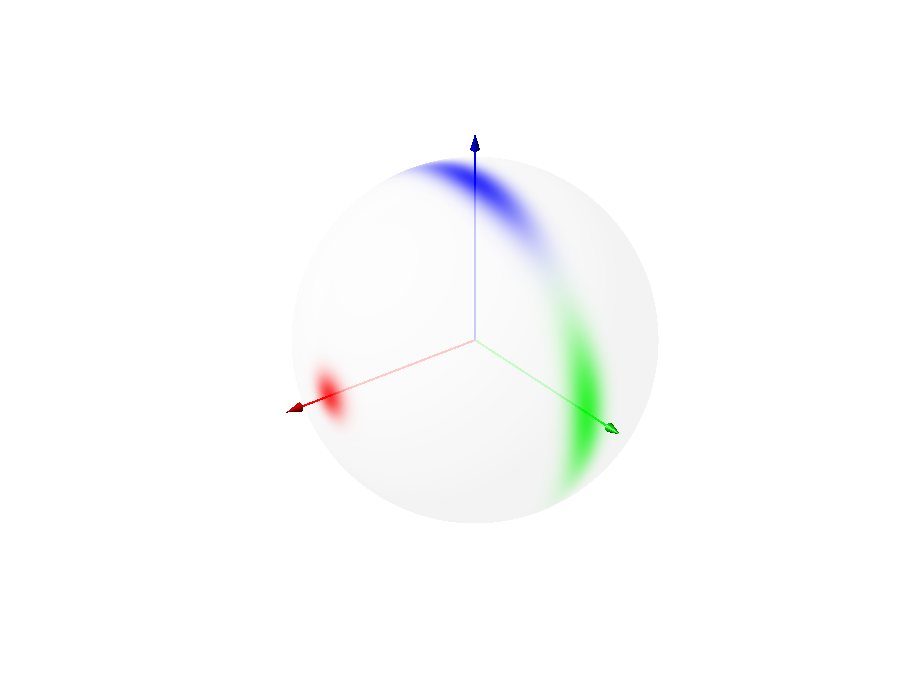
\includegraphics[trim=100 70 100 30, clip, scale=0.65]{figures/observability/prop_R_1}};
		\node at (7.5,5) {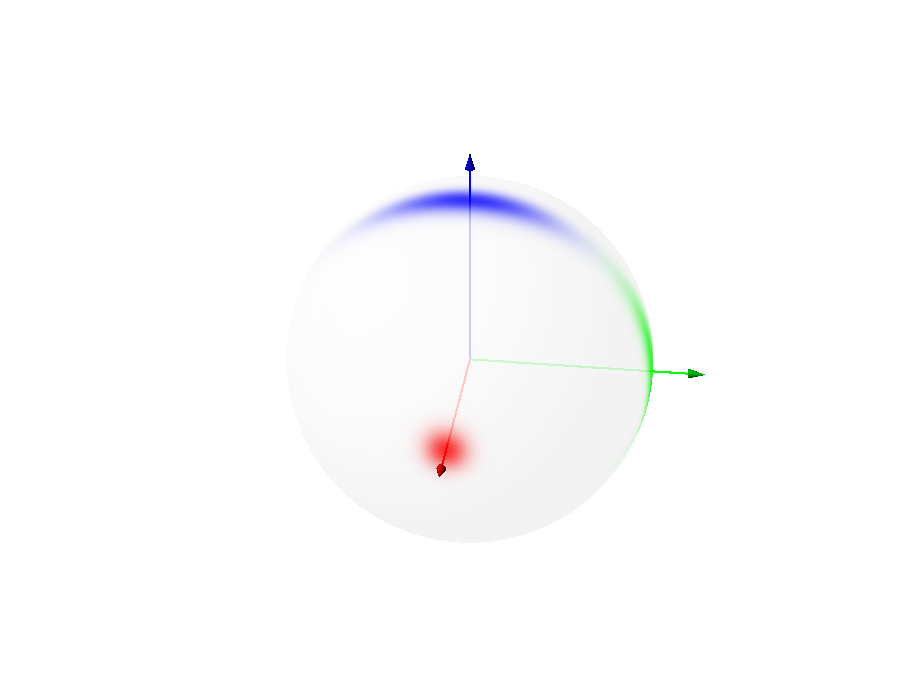
\includegraphics[trim=100 60 100 40, clip, scale=0.65]{figures/observability/prop_R_2}};
		\node at (12.5,5) {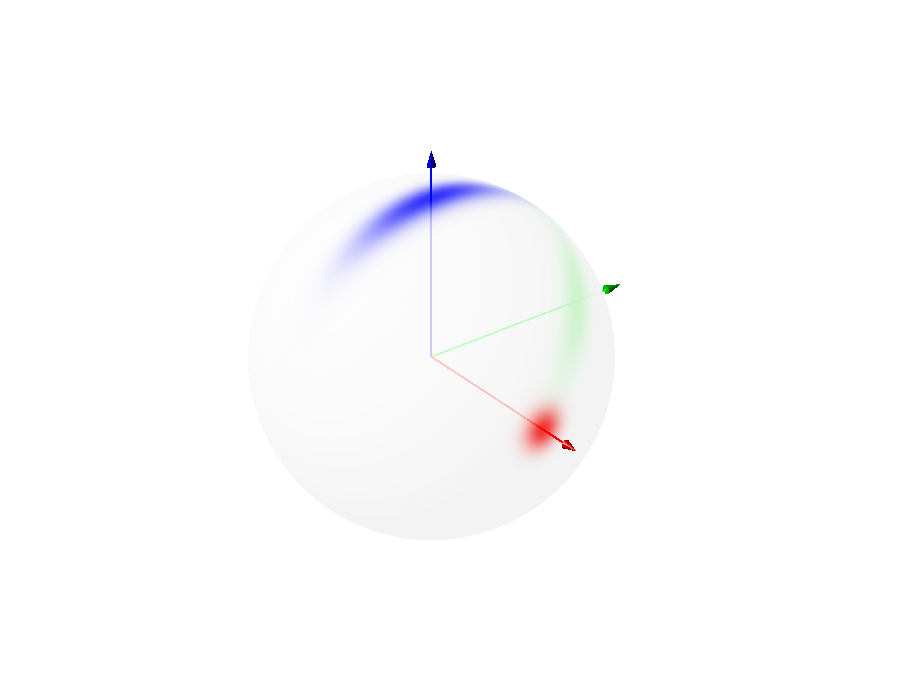
\includegraphics[trim=100 60 100 40, clip, scale=0.65]{figures/observability/prop_R_3}};
		
		\node at (2.5,0) {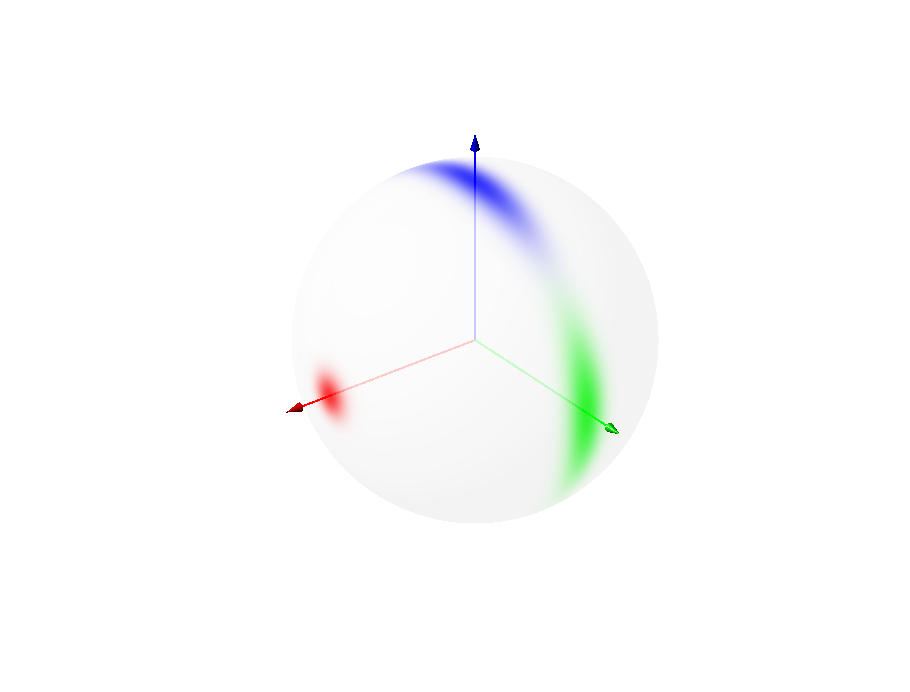
\includegraphics[trim=100 70 100 30, clip, scale=0.65]{figures/observability/prop_L_1}};
		\node at (7.5,0) {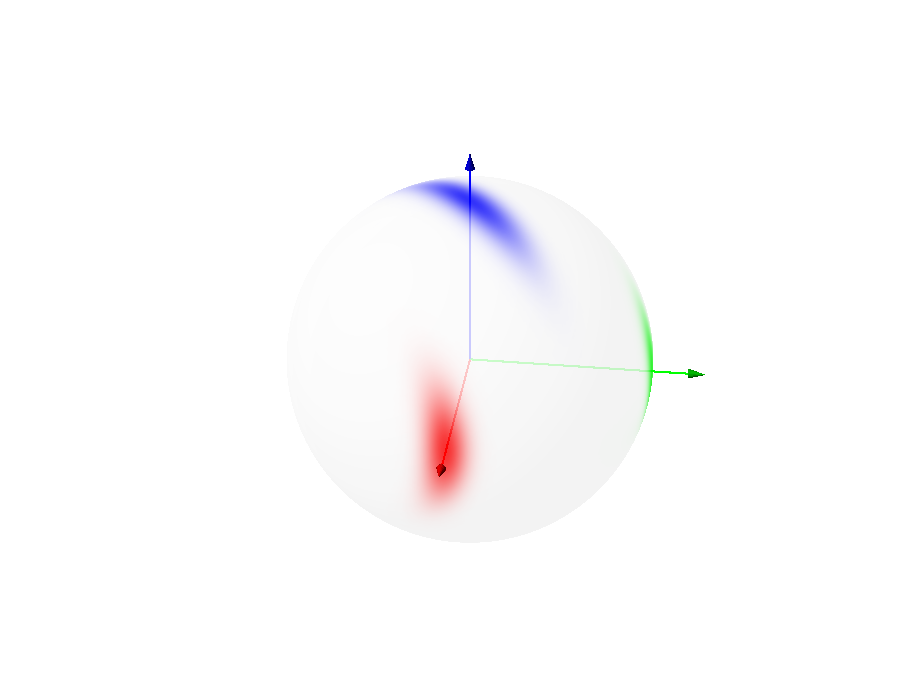
\includegraphics[trim=100 60 100 40, clip, scale=0.65]{figures/observability/prop_L_2}};
		\node at (12.5,0) {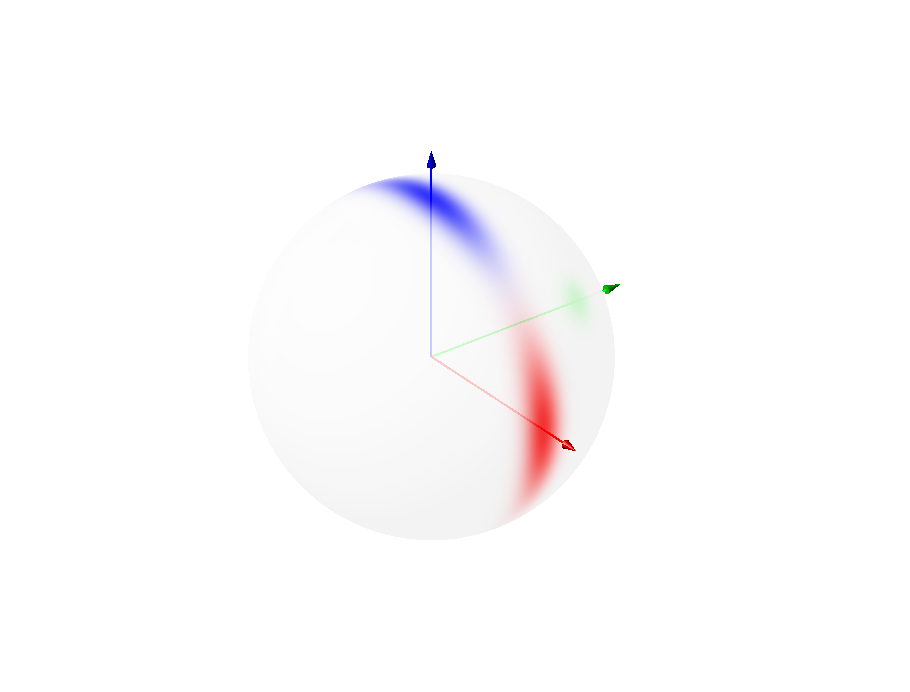
\includegraphics[trim=100 60 100 40, clip, scale=0.65]{figures/observability/prop_L_3}};
		
		\node at (0,4.85) {\rotatebox{90}{right-trivialized \eqref{eqn:observability-kinematics-right-dist}}};
		\node at (0,-0.3) {\rotatebox{90}{left-trivialized \eqref{eqn:observability-kinematics-left-dist}}};
		
		\draw[arrows={-Triangle[angle=30:8pt]}] (5.25,2.7) -- ++(90:0.8);
		\draw[arrows={-Triangle[angle=30:8pt]}] (5.25,2.7) -- ++(-30:0.8);
		\draw[arrows={-Triangle[angle=30:8pt]}] (5.25,2.7) -- ++(210:0.8);
		\node at (4.35,2.3) {$\bm{e}_1$};
		\node at (6.25,2.3) {$\bm{e}_2$};
		\node at (5.25,3.7) {$\bm{e}_3$};
		
		\node at (0.8,6.5) {(a)};
		\node at (5.8,6.5) {(b)};
		\node at (10.8,6.5) {(c)};
		\node at (0.8,1.55) {(d)};
		\node at (5.8,1.55) {(e)};
		\node at (10.8,1.55) {(f)};
		
		\node at (2.8,-3.0) {$t=0$s};
		\node at (7.7,-3.0) {$t=0.5$s};
		\node at (12.3,-3.0) {$t=1$s};
	\end{tikzpicture}

	\caption{Illustration of propagated uncertainties: (a-c) by the right-trivialized \eqref{eqn:observability-kinematics-right-dist}; (d-f) by the left-trivialized \eqref{eqn:observability-kinematics-left-dist}.
		The initial distribution is $R_0 \sim \mathcal{M}(F_0)$ with $F_0 = \diag(150, 10, 0)$.
		The angular velocities are $\omega = \Omega = \tfrac{\pi}{2}e_3 \SI{}{\radian\per\second}$ without any noise, which can be transformed to each other by the initial mean attitude $I_{3\times 3}$.
		The red, green and blue arrows represent the mean directions of the body-fixed $\bm{b}_1$, $\bm{b}_2$, $\bm{b}_3$ axes, and the corresponding shades represent the marginal distribution for each body-fixed axis.
		It can be observed that the mean attitude and the degree of dispersion are consistent between \eqref{eqn:observability-kinematics-right-dist} and \eqref{eqn:observability-kinematics-left-dist}.
		However, for \eqref{eqn:observability-kinematics-right-dist}, the most uncertain direction is fixed along the body-fixed $\bm{b}_1$ axis (red), but it is rotated in the inertial frame; and the most uncertain direction for \eqref{eqn:observability-kinematics-left-dist} is rotated in the body-fixed frame (from red to green), but it remains fixed along the inertial $\bm{e}_1$ axis, thereby causing all of the shades circular about $\bm{e}_1$.
	}
	\label{fig:observability-kinematics}
\end{figure}

\subsection{Measurement Update} \label{section:observability-measurement}

This subsection examines how the single direction measurements \eqref{eqn:observability-measurement-inertial} and \eqref{eqn:observability-measurement-body} are used to update the uncertainty propagated from the previous time step.
The additional information in the direction measurement is injected into the prior uncertainty by calculating the conditional distribution $R|x$ or $R|y$, using Bayes' formula. 
\begin{theorem} \label{thm:F_post}
	Let $R\sim\mathcal{M}(F^-)$ be a prior distribution for a given $F^-\in\mathbb{R}^{3\times 3}$.
	Then, for the inertial direction measurement, the posterior distribution of the attitude conditioned by $x$ is also matrix Fisher with $R|x \sim \mathcal{M}(F_I^+)$, where the posterior matrix parameter $F_I^+\in\mathbb{R}^{3\times 3}$ is given by
	\begin{align}
		F_I^+ = F^- + \kappa a x^T.\label{eqn:observability-measurement-F_I}
	\end{align}
	And for the body-fixed direction measurement, the posterior distribution is $R|y \sim \mathcal{M}(F_B^+)$, where $F_B^+\in\mathbb{R}^{3\times 3}$ is given by
	\begin{align}
		F_B^+ = F^- + \kappa y b^T.\label{eqn:observability-measurement-F_B}
	\end{align}
\end{theorem}
\begin{proof}
	The proof for inertial direction measurement is given in Theorem 3.2 of \cite{lee2018bayesian}, and the body-fixed direction measurement can be derived similarly.
\end{proof}

\begin{figure}
	\centering
	\begin{tikzpicture}
		\node at (2.4,5.5) {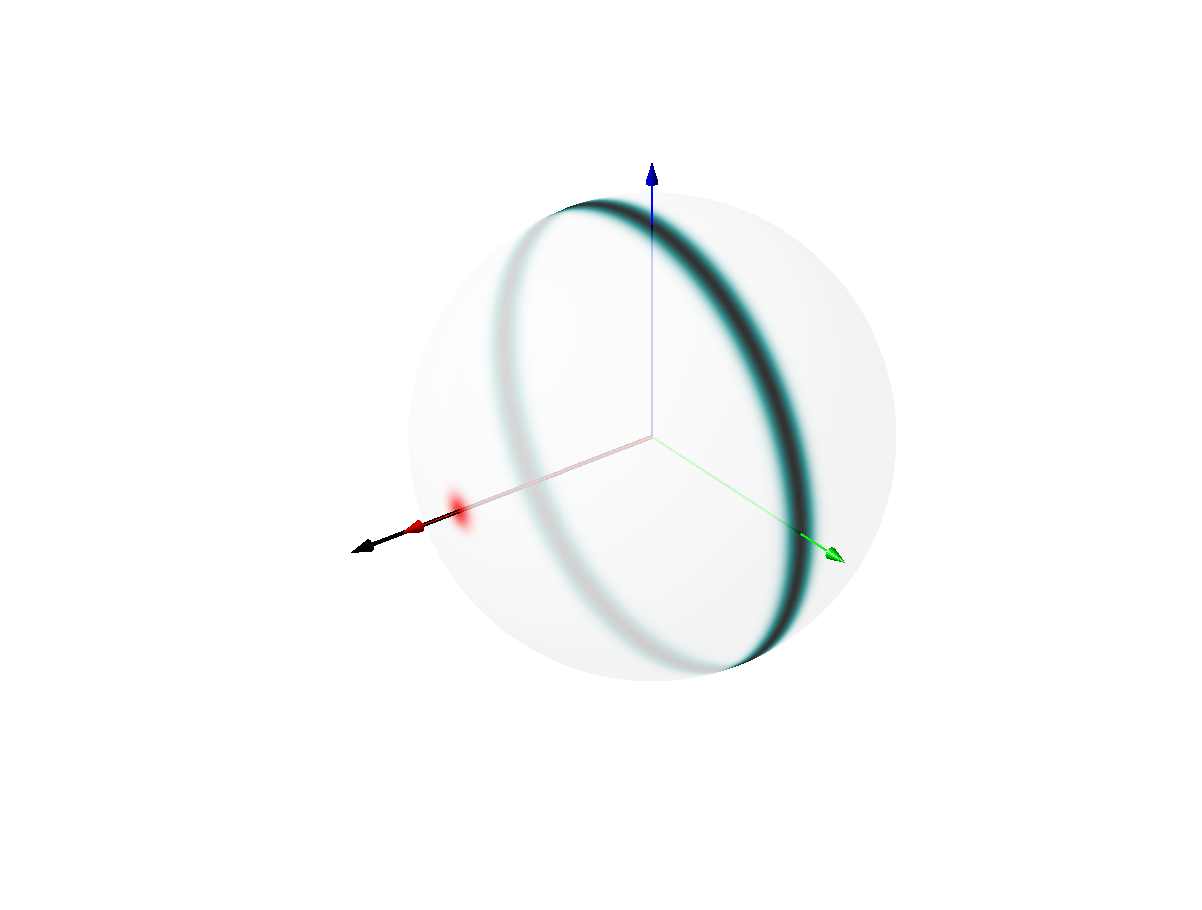
\includegraphics[trim=130 80 120 60, clip, scale=0.45]{figures/observability/mea_I_1}};
		\node at (7.3,5.5) {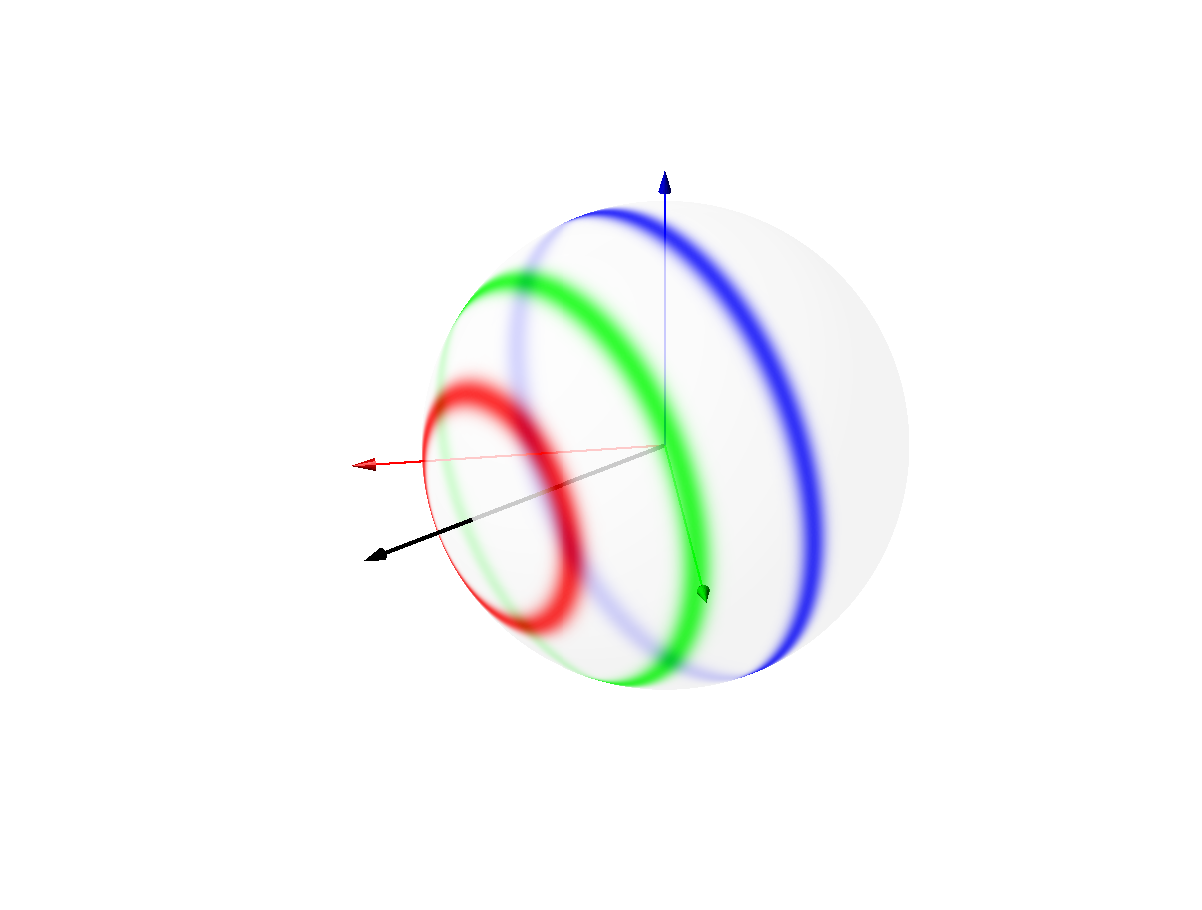
\includegraphics[trim=130 80 120 60, clip, scale=0.45]{figures/observability/mea_I_2}};
		\node at (12.1,5.5) {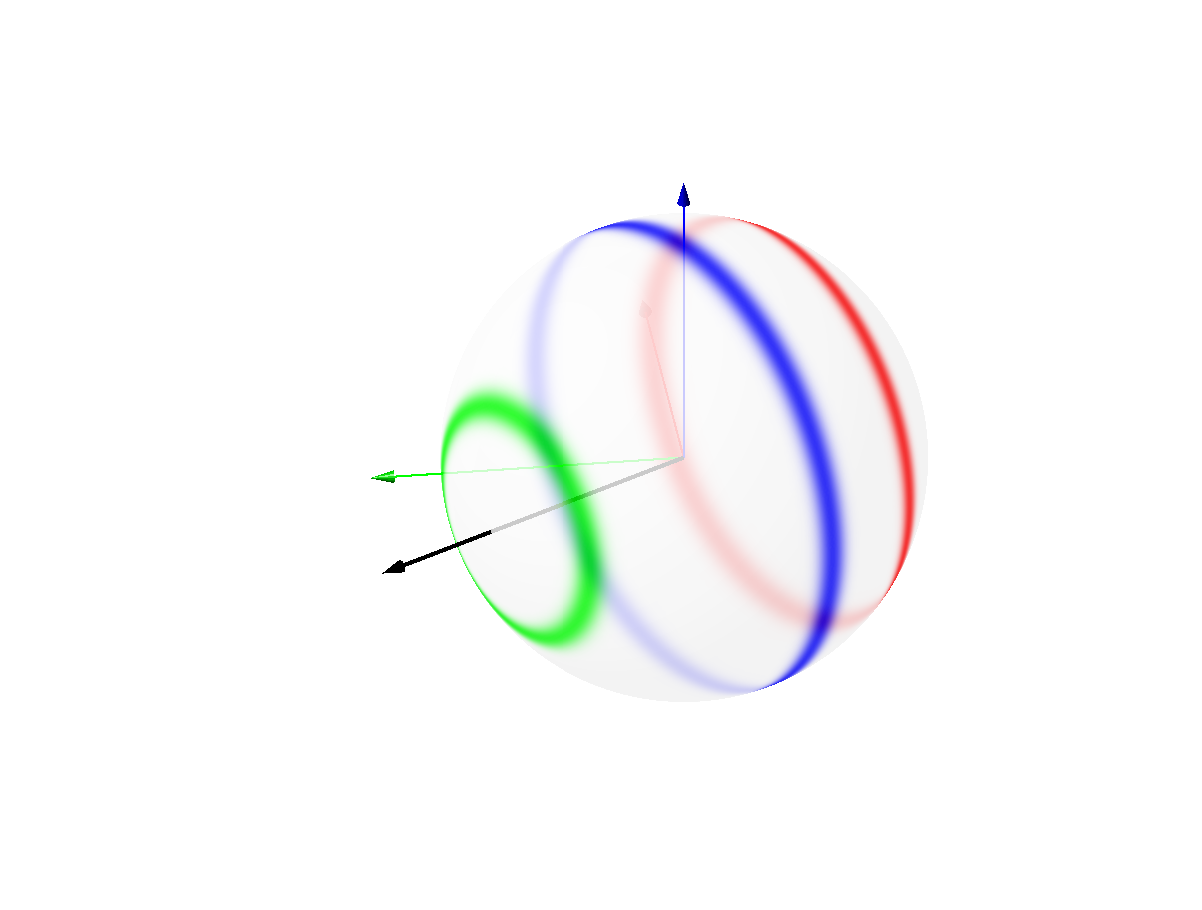
\includegraphics[trim=130 80 120 60, clip, scale=0.45]{figures/observability/mea_I_3}};
		
		\node at (2.7,0) {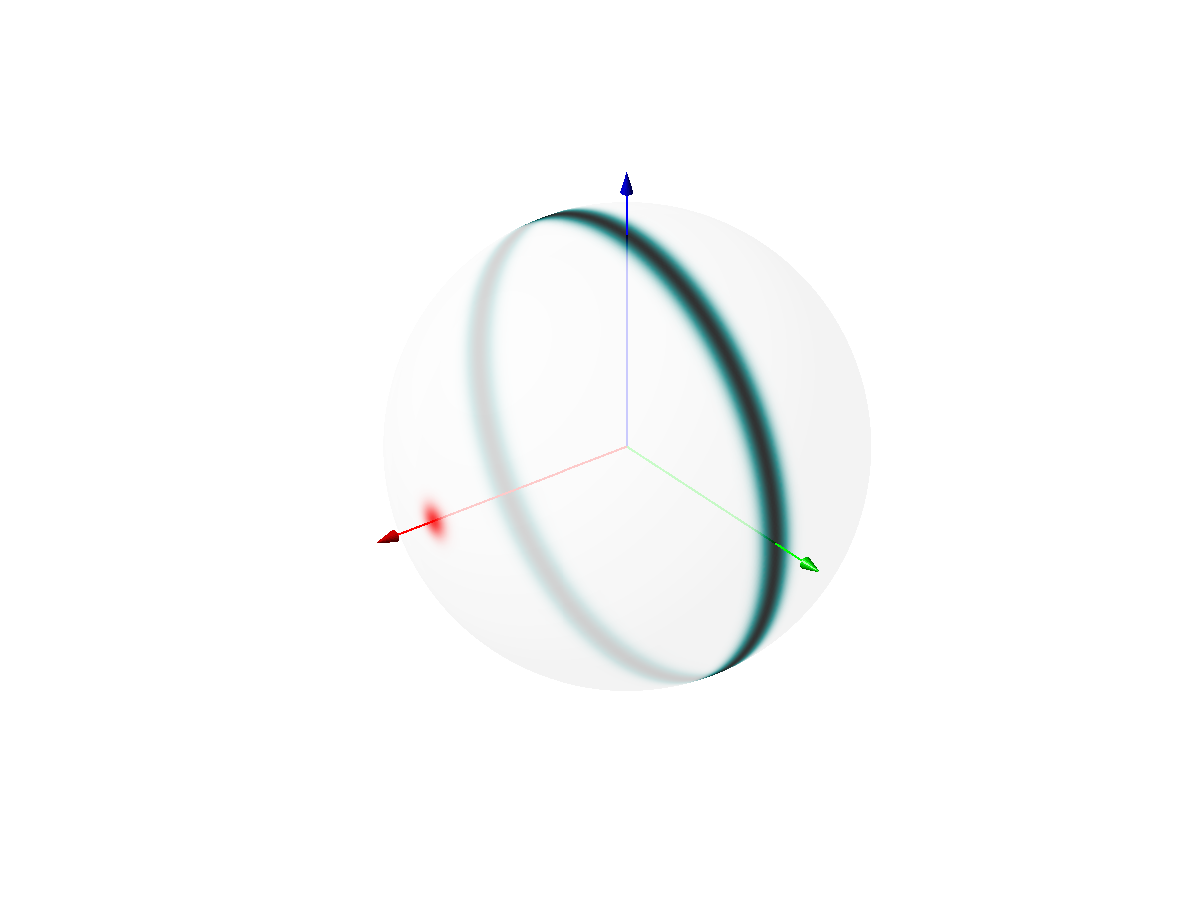
\includegraphics[trim=150 80 120 60, clip, scale=0.45]{figures/observability/mea_B_1}};
		\node at (7.8,0) {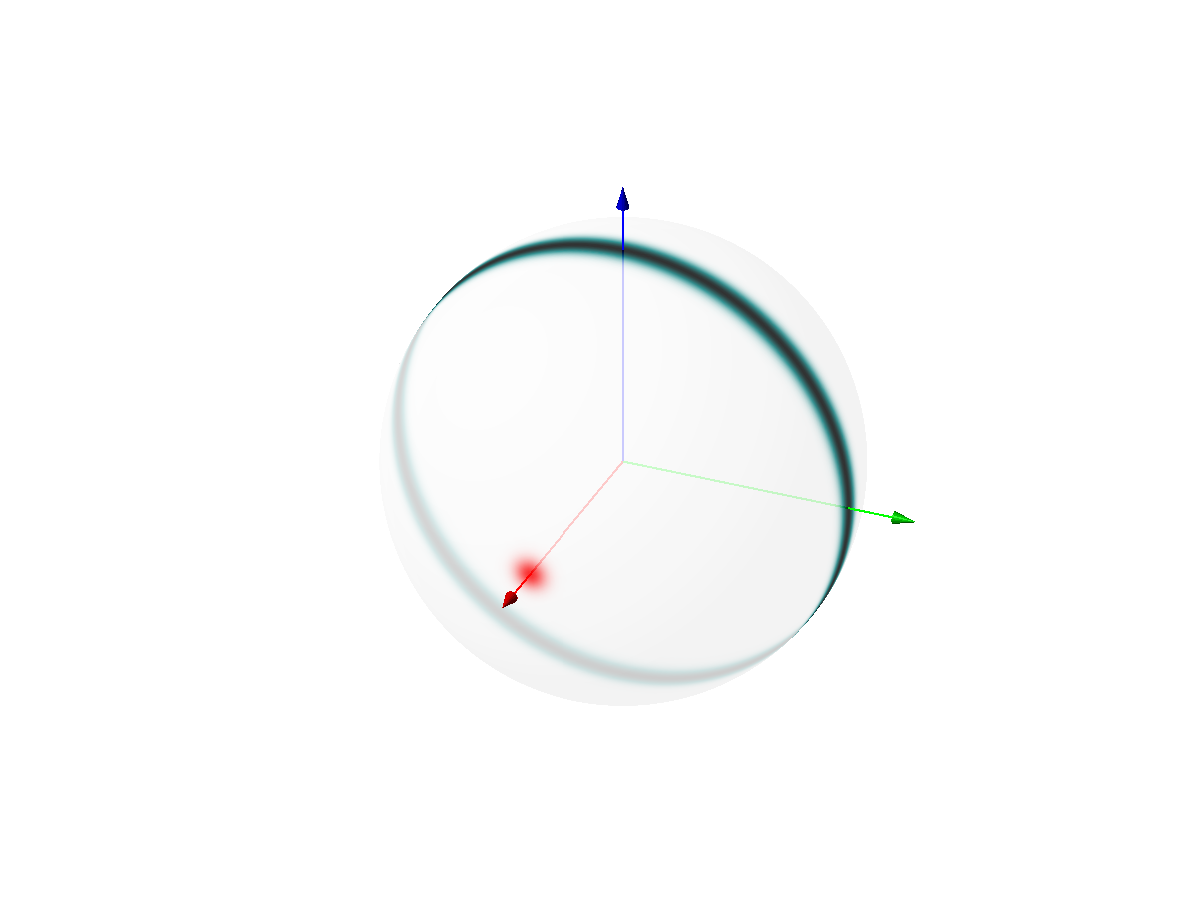
\includegraphics[trim=150 80 120 60, clip, scale=0.45]{figures/observability/mea_B_2}};
		\node at (12.8,0) {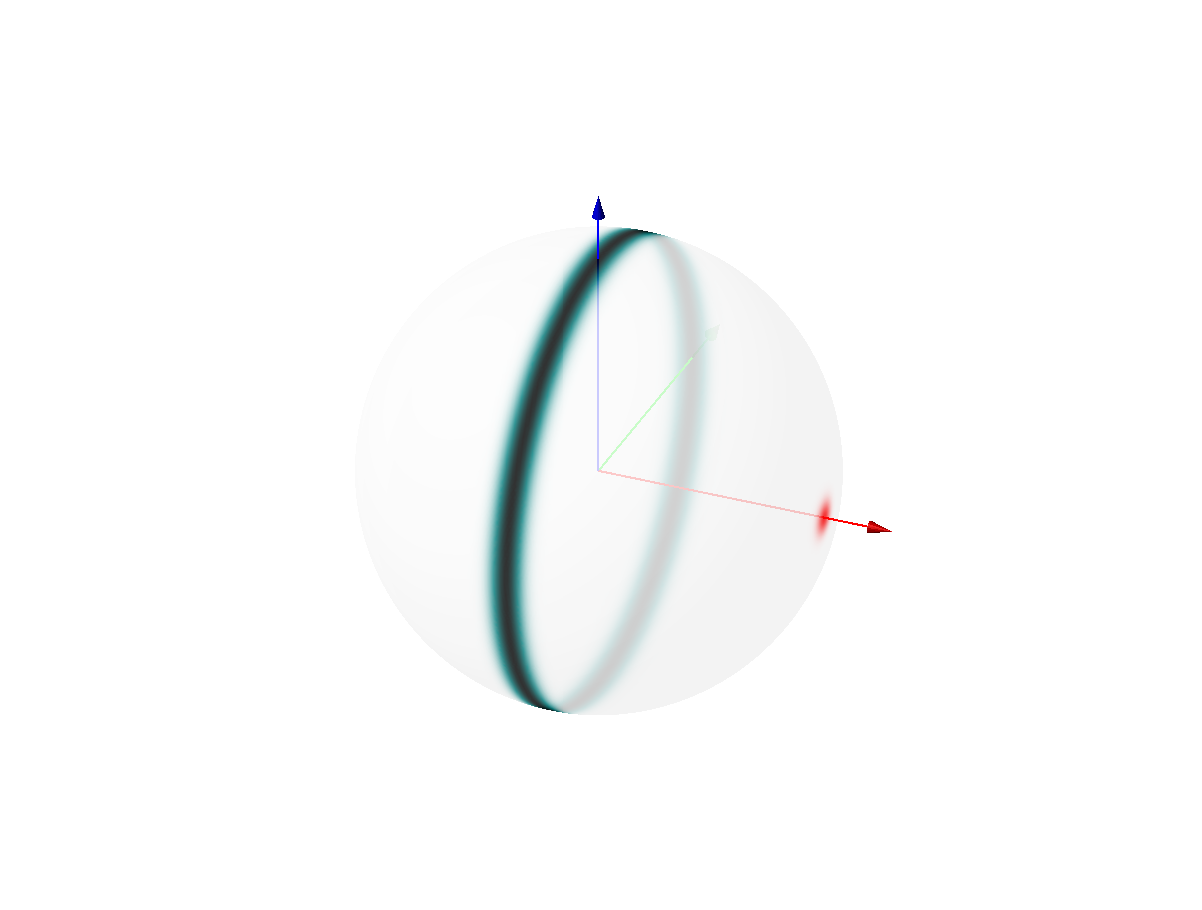
\includegraphics[trim=150 80 120 60, clip, scale=0.45]{figures/observability/mea_B_3}};
		
		\node at (0,5.5) {\rotatebox{90}{inertial dir. mea. \eqref{eqn:observability-measurement-inertial}}};
		\node at (0,0) {\rotatebox{90}{body-fixed dir. mea. \eqref{eqn:observability-measurement-body}}};
		
		\draw[arrows={-Triangle[angle=30:8pt]}] (5.25,-1.7) -- ++(90:0.8);
		\draw[arrows={-Triangle[angle=30:8pt]}] (5.25,-1.7) -- ++(-30:0.8);
		\draw[arrows={-Triangle[angle=30:8pt]}] (5.25,-1.7) -- ++(210:0.8);
		\node at (4.35,-2.1) {$\bm{e}_1$};
		\node at (6.25,-2.1) {$\bm{e}_2$};
		\node at (5.25,-0.7) {$\bm{e}_3$};
		
		\node at (0.8,7.2) {(a)};
		\node at (5.8,7.2) {(b)};
		\node at (10.8,7.2) {(c)};
		\node at (0.8,1.55) {(d)};
		\node at (5.8,1.55) {(e)};
		\node at (10.8,1.55) {(f)};
		
		\node at (2.8,2.6) {$x=e_1$};
		\node at (7.7,2.6) {$x=\tfrac{\sqrt{3}}{2}e_1 + \tfrac{1}{2}e_2$};
		\node at (12.6,2.6) {$x=-\tfrac{1}{2}e_1 + \tfrac{\sqrt{3}}{2}e_2$};
		
		\node at (2.8,-3.0) {$y=e_1$};
		\node at (7.7,-3.0) {$y=\tfrac{\sqrt{3}}{2}e_1 + \tfrac{1}{2}e_2$};
		\node at (12.6,-3.0) {$y=-\tfrac{1}{2}e_1 + \tfrac{\sqrt{3}}{2}e_2$};
	\end{tikzpicture}
	
	\caption{Posterior distribution with single direction measurements ($\kappa=500$): (a-c) inertial direction measurements \eqref{eqn:observability-measurement-inertial} with $a=e_1$; (d-f) body-fixed direction measurements \eqref{eqn:observability-measurement-body} with $b=e_1$.}
	\label{fig:observability-measurement}
\end{figure}

Next, the implications of \eqref{eqn:observability-measurement-F_I} and \eqref{eqn:observability-measurement-F_B} are studied.
Suppose that the attitude is completely unknown before the measurement, i.e., $F^-=0_{3\times 3}$. 
For the inertial direction measurement, the matrix parameter \eqref{eqn:observability-measurement-F_I} for the posterior distribution is decomposed into
\begin{align} \label{eqn:observability-measurement-SVD_FI}
	F_I^+  = \begin{bmatrix} a & a' & a'' \end{bmatrix} 
	\diag(\kappa, 0,0) \begin{bmatrix} x & x' & x'' \end{bmatrix}^T,
\end{align}
where $a',a''\in\Sph^2$ are arbitrarily chosen such that the matrix $[a,a',a'']\in\SO{3}$, and $x',x''\in\Sph^2$ are defined similarly.
Therefore, $F_I^+$ is written in the form of pSVD with $S=\diag(\kappa,0,0)$. 
The first principal axis is $a$ when resolved in the inertial frame, or $x$ when resolved in the body-fixed frame. 
Also, the rotation about the first principal axis is completely unknown as $s_2+s_3 = 0$.
More intuitively, the marginal distribution of each body-fixed axis makes a circle normal to $\bm{a}$ (the top row of Figure \ref{fig:observability-measurement}), which implies the rotation about $\bm{a}$ cannot be determined.
Since $\bm{a}$ is fixed in the inertial frame, the direction of this ambiguity is also fixed in the inertial frame regardless of the measurement.

Next, the matrix parameter \eqref{eqn:observability-measurement-F_B} for the posterior distribution of a body-fixed direction measurement is decomposed into
\begin{align} \label{eqn:observability-measurement-SVD_FB}
	F_B^+  = \begin{bmatrix} y & y' & y'' \end{bmatrix} 
	\mathrm{diag}[\kappa, 0,0] \begin{bmatrix} b & b' & b'' \end{bmatrix}^T,
\end{align}
where $y',y''\in\Sph^2$ and $b',b''\in\Sph^2$ are chosen such that the corresponding matrices in brackets belong to $\SO{3}$. 
The resulting first principal axis is $b$ when resolved in the body-fixed frame, or $y$ when resolved in the inertial frame.
The marginal distribution of each body-fixed axis makes a circle normal to $\bm{b}$ (the bottom row of Figure \ref{fig:observability-measurement}), about which the rotation cannot be determined.
Since $\bm{b}$ is fixed in the body-fixed frame, the direction of this ambiguity is also fixed to the body.

\subsection{Stochastic Observability Criterion}

To formally study the attitude observability with single direction measurements, here two stochastic attitude observability criteria are introduced.
Since the posterior distribution of $R$ conditioned by measurements contains all the information available to determine the attitude, we study:
(i) whether there is a \textit{unique} attitude that minimizes the mean square error for the posterior distribution,
and (ii) whether the Fisher information matrix for the mean attitude of $R$ is positive-definite when $R$ is distributed according to the matrix Fisher distribution.

One of the methods to estimate an attitude from a density function on $\SO{3}$ is to solve an optimization problem that minimizes the mean square Frobenius norm.
\begin{definition}
	Let $p(R)$ be the probability density function for a random $R\in\SO{3}$. 
	Its minimum mean square estimate (MMSE) is defined as
	\begin{align}
		\mathrm{M}_{\mathrm{MMSE}} [R] = \argmin_{Q\in\SO{3}} \{\expect{\| R - Q\|_F^2 }\},
	\end{align}
	where $\|\cdot \|_F$ denotes the Frobenius norm.
\end{definition}

Finding MMSE can be addressed in terms of pSVD as follows.

\begin{lemma} \label{lemma:observability-MMSE}
	Suppose $R\in\SO{3}$ is a random rotation matrix.
	Let the pSVD of its first moment be $\expect{R}=UDV^T$ with $D=\mathrm{diag}[d_1,d_2,d_3]$. 
	Depending on $D$, the MMSE of $R$ is given by
	\begin{enumerate}
		\item $d_2+d_3 >0$: $UV^T$ (unique),
		\item $d_1\neq d_2$ and $d_2+d_3=0$: $\{U\exp(\theta\hat e_1) V^T\,|\,\theta\in[-\pi,\pi)\}$ (1D),
		\item $d_1=d_2 = -d_3 >0$: $\{U\exp(\theta\hat a) V^T|\, a\in\Sph^2,\; a_3 =0, \theta\in[-\pi,\pi)\}$ (2D),
		\item $d_1=d_2=d_3=0$:  $\SO{3}$ (3D),
	\end{enumerate}
	where the number in the parentheses indicates the dimension of the set corresponding to the solution of MMSE.
\end{lemma}
\begin{proof}
	Let $\theta\in[-\pi,\pi)$ and $a\in\Sph^2$ be defined such that $U^T R V = \exp(\theta\hat a)$. 
	Then, it can be shown that
	\begin{align} \label{eqn:observability-trsRER}
		\tr{R^T \expect{R}} = \tr{D} - (1-\cos\theta) \sum_{i=1}^3 (d_i+d_j) a_k^2,
	\end{align}
	for $i\neq j\neq k$ and $i,j,k\in\{1,2,3\}$.
	Since $d_1+d_2 \geq d_3+d_1 \geq d_2 +d_3 \geq 0$, the above is maximized when $\theta=0$, or equivalently $R= UV^T$. 
	
	The uniqueness is contributed by two aspects: the uniqueness of $UV^T$ from the proper singular value decomposition and the uniqueness of the maximum at \eqref{eqn:trsRER}.
	First note that the non-uniqueness of proper singular vectors caused by any simultaneous sign change of the corresponding columns of $U$ and $V$ does not affect the uniqueness of $UV^T$, therefore only the non-uniqueness of $U,V$ caused by repeated singular values is considered.
	\begin{enumerate}
		\item $d_2+d_3 >0$:
		If $d_3\geq 0$, the polar decomposition of $\expect{R}$ is written as $\expect{R} = (UV^T) \cdot (VDV^T)$, where $VDV^T = (\expect{R}^T\expect{R})^{1/2}$ is uniquely determined.
		The rank of $VDV^T$ is at least two, so $UV^T$ rotates two independent columns of $VDV^T$ to the corresponding columns of $\expect{R}$, and therefore it is unique.
		
		Next, when $d_3<0$, consider two sub-cases: (i) if $d_1\neq d_2$, then both $U$ and $V$ are unique; (ii) if $d_1=d_2$, $(U,V)$ can be replaced by $(U\exp(\phi\hat{e}_3),V\exp(\phi\hat{e}_3))$ for any $\phi\in[-\pi,\pi)$, but $UV^T$ is still unique.
		\item[2a)] $d_1 \neq d_2 =  d_3 =  0$:  It can be shown that
		\begin{align*}
			\tr{R^T \expect{R}} & = \tr{D} - (1-\cos\theta) d_1 (1-a_1^2),
		\end{align*}
		which is maximized for any $R$ in the given set of $a=e_1$. 
		The matrices $U$ and $V$ can be replaced with 
		$U\exp(\phi_1\hat e_1)$ and $V\exp(\phi_2\hat e_1)$, respectively, for any $\phi_1,\phi_2\in[-\pi,\pi)$. 
		However, the ambiguity of $U,V$ does not enlarge the set of $R$ maximizing \eqref{eqn:observability-trsRER}.
		\item[2b)] $d_1 \neq d_2 = -d_3 >0$: Similarly, \eqref{eqn:observability-trsRER} is maximized for any $R$ in the given set.
		The matrices $(U,V)$ can be replaced with 
		$(U\exp(\phi\hat e_1), V\exp(-\phi\hat e_1))$ for any $\phi\in[-\pi,\pi)$.
		But, it does not alter the given set. 
		\item[3)] $d_1 = d_2 = -d_3 >0$: It can be shown that
		\begin{align*}
			\tr{R^T \expect{R}} = \tr{D} - (1-\cos\theta)(d_1+d_2)a_3^2,
		\end{align*}
		which is maximized when $a_3=0$. 
		The ambiguity of $U$ and $V$ is written as $U\exp(\phi_1\hat e_1+\phi_2 \hat e_2 +\phi_3 \hat e_3)$ and $V\exp(-\phi_1\hat e_1 - \phi_2\hat e_2 +\phi_3\hat e_3)$, respectively for any $\phi_1,\phi_2,\phi_3\in[-\pi,\pi)$.
		Same as above, this does not alter the set of $R$ maximizing \eqref{eqn:observability-trsRER}.
		\item[4)] $d_1 = d_2=d_3=0$: This is a trivial case when $\tr{R^T \expect{R}}=0$ for any $R\in\SO{3}$.
	\end{enumerate}
	These complete the proof.
\end{proof}

For all cases, the set of MMSE contains $UV^T$.
Nevertheless, only when $d_2+d_3>0$, the MMSE is unique.
Otherwise, it can only be determined up to a rotation, where the dimension of the set representing the solution of MMSE is equivalent to 3 minus the rank of $\tr{D}I_{3\times 3}-D = \diag(d_2+d_3, d_1+d_3, d_1+d_2)$.
Therefore, it is claimed that the attitude is completely observable given a density function on $\SO{3}$ if $\tr{D}I_{3\times 3}-D$ is positive-definite, i.e., when the MMSE is unique.

The above observability criterion is solely based on the first moment, and therefore, it can be applied to an unknown attitude following an arbitrary distribution. 
Next, it is assumed that the attitude is distributed according to a matrix Fisher distribution to present an alternative information theoretic observability criterion.

Suppose $R\sim \mathcal{M}(F)$ where the pSVD of $F\in\mathbb{R}^{3\times 3}$ is given by $F=USV^T$.
As discussed in Chapter \ref{section:MF-MF}, the MMSE of $R\sim\mathcal{M}(USV^T)$ is given by the mean attitude $R^*=UV^T$, and we want to calculate its Fisher information $\mathbb{I}(R^*)$.
To do this, first a more general problem of estimating $U$, $S$, and $V$ from the given samples of $R$ is studied.
The log-likelihood is
\begin{align} \label{eqn:observability-FIM-likelihood}
	l(R|U,S,V) = \tr{USV^T R^T} - \log c(S).
\end{align}
And the corresponding Fisher information matrix is calculated as follows~\cite{smith2005covariance}.

\begin{lemma} \label{lemma:observability-FIM}
	The Fisher information matrix of \eqref{eqn:observability-FIM-likelihood}, namely $\mathbb{I}(U,S,V):\mathbb{R}^9\times\mathbb{R}^9\rightarrow \mathbb{R}$ is constructed as 
	\begin{align} \label{eqn:observability-FIM}
		\mathbb{I} (U,S,V) &= -\expect{ \nabla^2 l (R|U,S,V) }\nonumber \\
		&=\begin{bmatrix}
			\tr{DS}I_{3\times 3}- DS  & 0 & \sum_{i=1}^3 e_i^T s \hat e_i D\hat e_i \\
			0 & \frac{\partial^2 \log c(S)}{\partial s^2} & 0 \\
			\sum_{i=1}^3 e_i^T s \hat e_i D\hat e_i& 0 & \tr{DS}I_{3\times 3} -DS
		\end{bmatrix},
	\end{align}
	where $D\in\mathbb{R}^{3\times 3}$ is the diagonal matrix composed of the proper singular values of $\expect{R|U,S,V}$, $S = \diag(s_1, s_2, s_3)$, and $\nabla^2$ is the covariant Hessian on $\SO{3}\times\mathbb{R}^3\times\SO{3}$.
\end{lemma}
\begin{proof}
	Let $\mathsf{Q} = \SO{3}\times\mathbb{R}^3\times\SO{3}$, and $q=(U,S,V)\in\mathsf{Q}$.
	The tangent space $\mathsf{T}_q\mathsf{Q}$ is identified with $\mathsf{T}_q\mathsf{Q}\simeq \mathbb{R}^9$ through the hat map, and the cotangent space is also identified with $\mathbb{R}^9$ using the dot product.
	More specifically, for $\xi=(u,\varsigma,v)\in\mathbb{R}^9$, the corresponding tangent vector is given by $(U\hat u, \varsigma, V\hat v)\in\mathsf{T}_q \mathsf{Q}$. 
	
	Since $l$ is a real-valued function on $\mathsf{Q}$, its covariant derivative $\nabla_\xi l$ along $\xi$ is equivalent to the differential $dl(\xi)$ given by
	\begin{align*}
		&\nabla_\xi l = \frac{d}{d\epsilon}\bigg|_{\epsilon =0} l( R | U\exp(\epsilon\hat u), S+\epsilon\mathrm{diag}[\varsigma], V\exp(\epsilon\hat v))\\
		& = \tr{(U\hat uSV^T + U\mathrm{diag}[\varsigma]V^T - US\hat v V^T)^TR} - \frac{\partial \log c(S)}{\partial s}\cdot \varsigma \\
		& = 
		\begin{bmatrix}
			(QS-SQ^T)^\vee \\ 
			\mathrm{diag}[Q]-\frac{1}{c(S)} \frac{\partial c(S)}{\partial s} \\
			(Q^TS - SQ)^\vee
		\end{bmatrix}\cdot \xi,
	\end{align*}
	where $Q=U^TRV$.
	Because $\expect{Q} = D$ is diagonal, it is straightforward to show $\expect{dl(\xi)}=0$ for any $\xi\in\mathbb{R}^9$.
	
	The covariant Hessian of $l$ along $\xi_1$ and $\xi_2$ is given by $\nabla^2_{\xi_1,\xi_2} l = \xi_2(\xi_1 l) - (\nabla_{\xi_2}\xi_1) l = \xi_2 ( dl(\xi_1)) - dl(\nabla_{\xi_2} \xi_1)$,
	where the second term vanishes after taking expectation.
	The first term is bi-linear in $\xi_1$ and $\xi_2$, thus it can be written as a matrix as in \eqref{eqn:observability-FIM}.
	Suppose $\xi_1 = (u_1,0,0)$ and $\xi_2 =(u_2,0,0)$, then it can be shown that
	\begin{align*}
		\xi_2 (dl(\xi_1)) = (-\hat u_2 QS -SQ^T \hat u_2)^\vee \cdot u_1 = u_1^T \left\{\frac{1}{2}(QS+SQ^T) - \tr{QS}I_{3\times 3}\right\} u_2.
	\end{align*}
	Taking the expectation of the expression in the braces with $\expect{Q}=D$ and multiplying it with $-1$ yield the upper-left 3-by-3 block of \eqref{eqn:observability-FIM}.
	The remaining blocks can be obtained similarly.
\end{proof}

Next, the Fisher information $\mathbb{I}(R^*)$ can be obtained with the above information matrix.
Since the variations of $U$ and $V$ are written as $\delta U = U\hat u$ and $\delta V= V\hat v$ for $u,v\in\mathbb{R}^3$, it can be shown that
\begin{align*}
	\delta R^* = U\hat u V^T - U\hat vV^T.
\end{align*}
Let $\eta = u-v\in\mathbb{R}^3$ so that $\delta R^* = U\hat\eta V^T$.
Thus, the Fisher information matrix for the mean attitude $R^*$ is constructed by left-multiplying \eqref{eqn:observability-FIM} with the matrix $\frac{1}{2} [I_{3\times 3}; 0_{3\times 3}; -I_{3\times 3}]$, and by right-multiplying \eqref{eqn:observability-FIM} with its transpose, to obtain
\begin{align}
	\mathbb{I}(R^*) = \frac{1}{2} \mathrm{diag} \!
	\begin{bmatrix} (d_2+d_3)(s_2+s_3) \\ (d_3+d_1)(s_3+s_1) \\ (d_1+d_2)(s_1+s_2) \end{bmatrix}.\label{eqn:FIM_eta}
\end{align}
According to the Cram\'{e}r--Rao inequality, the inverse of Fisher information $\mathbb{I}(R^*)$ is a lower bound of the variance of all unbiased estimates, up to additional curvature terms.
Therefore, its positive-definiteness can be used to define observability \cite{mohler1988nonlinear}.
Interestingly, by Lemma \ref{lemma:MF-SD}, the positive-definiteness of $\mathbb{I}(R^*)$ is equivalent to the uniqueness of MMSE presented in Lemma \ref{lemma:observability-MMSE}.
Based on these results, we formulate stochastic attitude observability for an arbitrary density as follows.
\begin{definition} \label{def:observability}
	A random rotation matrix $R\sim p(R)$ is stochastically observable if $d_2+ d_3 >0$, or equivalently
	\begin{align}
		\mathcal{O} = \tr{D}I_{3\times 3} - D \succ 0,\label{eqn:OC}
	\end{align}
	where $D=\mathrm{diag}[d_1,d_2,d_3]$ is the proper singular values of $\expect{R}$.  
	The corresponding measure of observability is
	\begin{align}
		\rho(R) = \det[\mathcal{O}] = (d_1+d_2)(d_3+d_1)(d_2+d_3).
	\end{align}
\end{definition}
When $R\sim\mathcal{M}(USV^T)$, it is straightforward to show that \eqref{eqn:OC} is equivalent to $\tr{S}I_{3\times 3} - S\succ 0$ with Lemma \ref{lemma:MF-SD}.
Note that these are readily applied to the stochastic observability considered in this section, as the posterior distribution conditioned by direction measurements is assumed to be a matrix Fisher distribution according to Theorem \ref{thm:F_post}, which is presented in the next subsection.

\subsection{Attitude Observability Results}

The attitude uncertainty propagation in Chapter \ref{section:observability-propagation}, and the measurement update in Chapter \ref{section:observability-measurement} constitute a Bayesian estimator, which provides the posterior distribution of the attitude conditioned by the history of direction measurements.
The posterior distribution can then be used in Definition \ref{def:observability} to determine attitude observability.
As there are two cases for each of uncertainty propagation and measurement update, there are four possible combinations as summarized in Table \ref{table:observability}.
This subsection identifies two combinations that yield unobservability, and two other cases resulting in observability with single direction measurements.
The same results can also be derived in a deterministic sense as presented in Appendix \ref{app:obervability-deterministic}.

We first discuss why the common IMU cannot estimate the full attitude with single direction measurements.
In a typical IMU, the angular velocity is measured in the body-fixed frame using a gyroscope, and the reference direction in the inertial frame, such as the direction of gravity, is measured in the body-fixed frame. 
As such it is a combination of the left-trivialized \eqref{eqn:observability-kinematics-left-dist} and the inertial direction measurement \eqref{eqn:observability-measurement-inertial}.
Looking at the bottom row of Figure \ref{fig:observability-kinematics} and the top row of Figure \ref{fig:observability-measurement}, it is clear why the attitude cannot be determined in this case: the direction about which the rotation cannot be determined, namely the first principal axis, remains unchanged in the inertial frame for both \eqref{eqn:observability-kinematics-left-dist} and \eqref{eqn:observability-measurement-inertial}.
This is formulated in the next theorem.

\begin{theorem} \label{thm:observability-nonobs}
	Consider the two Bayesian attitude estimators for
	\begin{itemize}
		\item right-trivialized angular velocity in the inertial frame  \eqref{eqn:observability-kinematics-right-dist} and body-fixed direction measurement \eqref{eqn:observability-measurement-body}  
		\item left-trivialized angular velocity in the body-fixed frame \eqref{eqn:observability-kinematics-left-dist}, and inertial direction measurement \eqref{eqn:observability-measurement-inertial} 
	\end{itemize}
	with the initial distribution $F_0=0_{3\times 3}$.
	For both cases, the attitude is not observable.
\end{theorem}
\begin{proof}
	First consider the filter given by \eqref{eqn:observability-kinematics-UV_R}, \eqref{eqn:observability-kinematics-S}, and \eqref{eqn:observability-measurement-F_B}.
	The propagated uncertainty before the first measurement is $F_1^- = 0_{3\times 3}$, thus $F_1 = \kappa y_1b^T$ after conditioning the first measurement.
	As shown in \eqref{eqn:observability-measurement-SVD_FB}, $(s_2)_1=(s_3)_1=0$, and $V_1e_1 = b$.
	We proceed with induction.
	Suppose $(s_2)_k=(s_3)_k=0$, and $V_ke_1 = b$.
	Then by \eqref{eqn:observability-kinematics-UV_R}, \eqref{eqn:observability-kinematics-S} and Lemma \ref{lemma:MF-SD}, the propagated parameters before the next measurement still satisfy $(s_2)_{k+1}^-=(s_3)_{k+1}^- = 0$ and $V_{k+1}^-e_1=b$.
	Next consider the update $F_{k+1} = F_{k+1}^-+\kappa y_{k+1}b^T$, which can be written as
	\begin{align*}
		F_{k+1} = \left((s_1)_{k+1}^-U_{k+1}^-e_1 + \kappa y_{k+1}\right)b^T \triangleq ub^T,
	\end{align*}
	where $u\in\mathbb{R}^3$.
	Let $U_{k+1} = \Big[ \frac{u}{\norm{u}}, u', u'' \Big]$, where $u',u''\in\Sph^2$ are arbitrarily chosen such that $U_{k+1}\in\SO{3}$.
	Also let $S_{k+1} = \diag(\norm{u},0,0)$, and $V_{k+1} = [ b, b', b'' ]$ as in \eqref{eqn:observability-measurement-SVD_FB}.
	Then $F_{k+1} = U_{k+1}S_{k+1}V_{k+1}^T = ub^T $ is the pSVD of $F_{k+1}$, and it has been shown that $(s_2)_{k+1}=(s_3)_{k+1}=0$ and $V_{k+1}e_1=b$.
	Therefore, $(s_2)_k=(s_3)_k=0$ for all $k\in\mathbb{N}$, and by Lemma \ref{lemma:MF-SD}, the attitude is not observable.
	The proof for the second case is similar.
\end{proof}

Next, two examples illustrating that the other two combinations yield observability are presented.
Consider the combination of right-trivialized \eqref{eqn:observability-kinematics-right-dist} and inertial direction measurement \eqref{eqn:observability-measurement-inertial} for a specific case where the true attitude evolves according to
\begin{align}
	R(t) = R_0 \exp(\hat\Omega t) = \exp(\hat\omega t) R_0,\label{eqn:R_est}
\end{align}
with $R_0=I_{3\times 3}$ and $\Omega = \omega = -\frac{\pi}{2\sqrt{3}}[1, 1, 1]\in\mathbb{R}^3$. 
Initially, it is assumed that the attitude is completely unknown, i.e., $F_0 = 0_{3\times 3}$, as illustrated in Figure \ref{fig:observability-est_RI}(a).
Then after updated by an inertial direction measurement with $a = e_1$, the rotation about the reference direction is unobservable and the resulting distribution is axially symmetric about $\mathbf{e}_1$ (Figure \ref{fig:observability-est_RI}(b)).
For the right-trivialized \eqref{eqn:observability-kinematics-right-dist}, the distribution rotates in the inertial frame over the propagation, and therefore, the direction of ambiguity is no longer along $\bm{e}_1$ (Figure \ref{fig:observability-est_RI}(c)(d)).
The next inertial direction measurement is fixed in the inertial frame along $\bm{e}_1$ (Figure \ref{fig:observability-est_RI}(e)).
Thus, it resolves the ambiguity of the propagated density to determine the attitude completely (Figure \ref{fig:observability-est_RI}(f)).

The other combination of left-trivialized \eqref{eqn:observability-kinematics-left-dist} and body-fixed direction measurement \eqref{eqn:observability-measurement-body} is similar.
The direction of ambiguity caused by the first body-fixed direction measurement with $b=e_1$ is fixed in the inertial frame after propagation (Figure  \ref{fig:observability-est_LB}(d)).
However, the ambiguous direction of the next direction measurement is rotated in the inertial frame (Figure \ref{fig:observability-est_LB}(e)), and this resolves the previous ambiguity (Figure \ref{fig:observability-est_LB}(f)).
The above intuition is formally presented in the next theorem.

\begin{figure}
	\centering
	\begin{tikzpicture}
		\node at (2.5,5.5) {
\includegraphics[trim=150 80 120 60, clip, scale=0.45]{figures/observability/est_RI_F1_prior}};
		\node at (7.5,5.5) {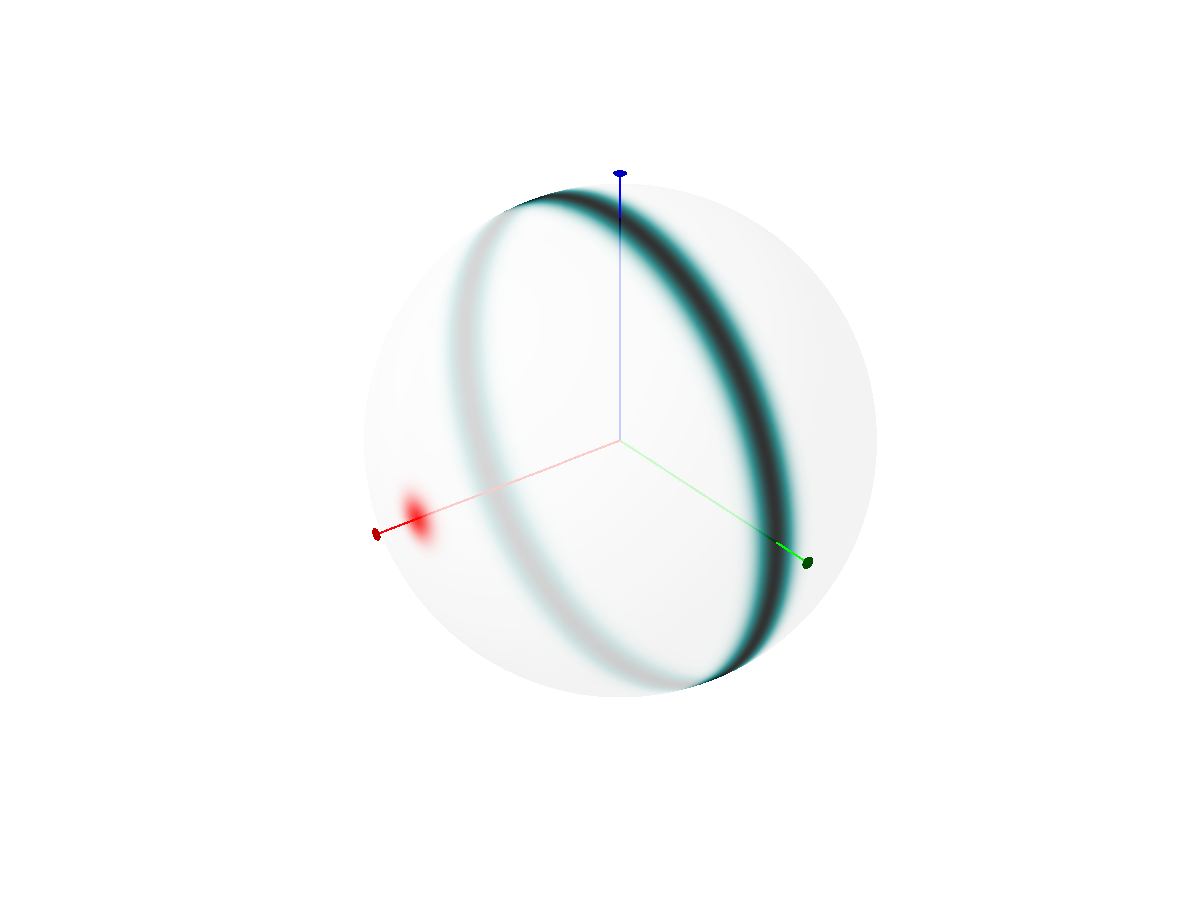
\includegraphics[trim=150 80 120 60, clip, scale=0.45]{figures/observability/est_RI_F1}};
		\node at (12.5,5.5) {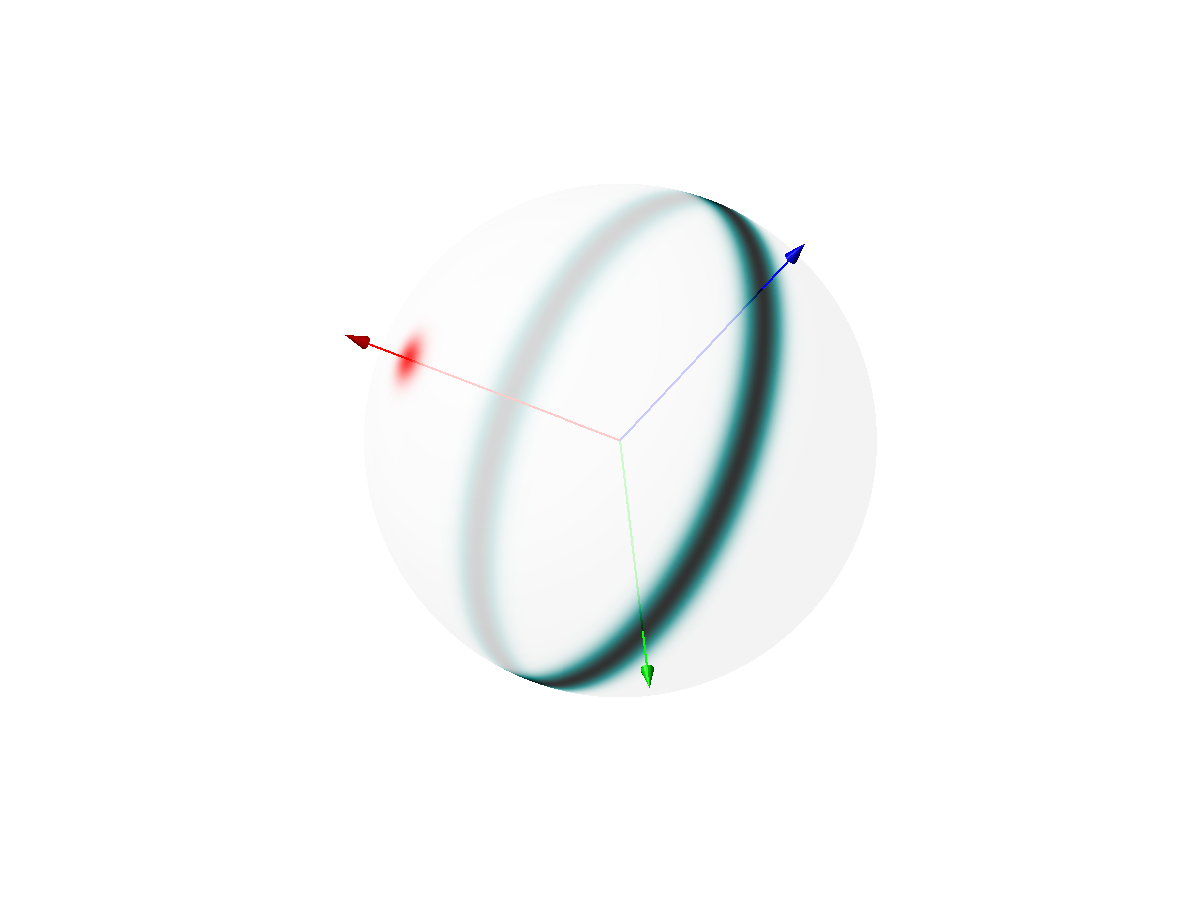
\includegraphics[trim=150 80 120 60, clip, scale=0.45]{figures/observability/est_RI_F3}};
		
		\node at (2.5,0) {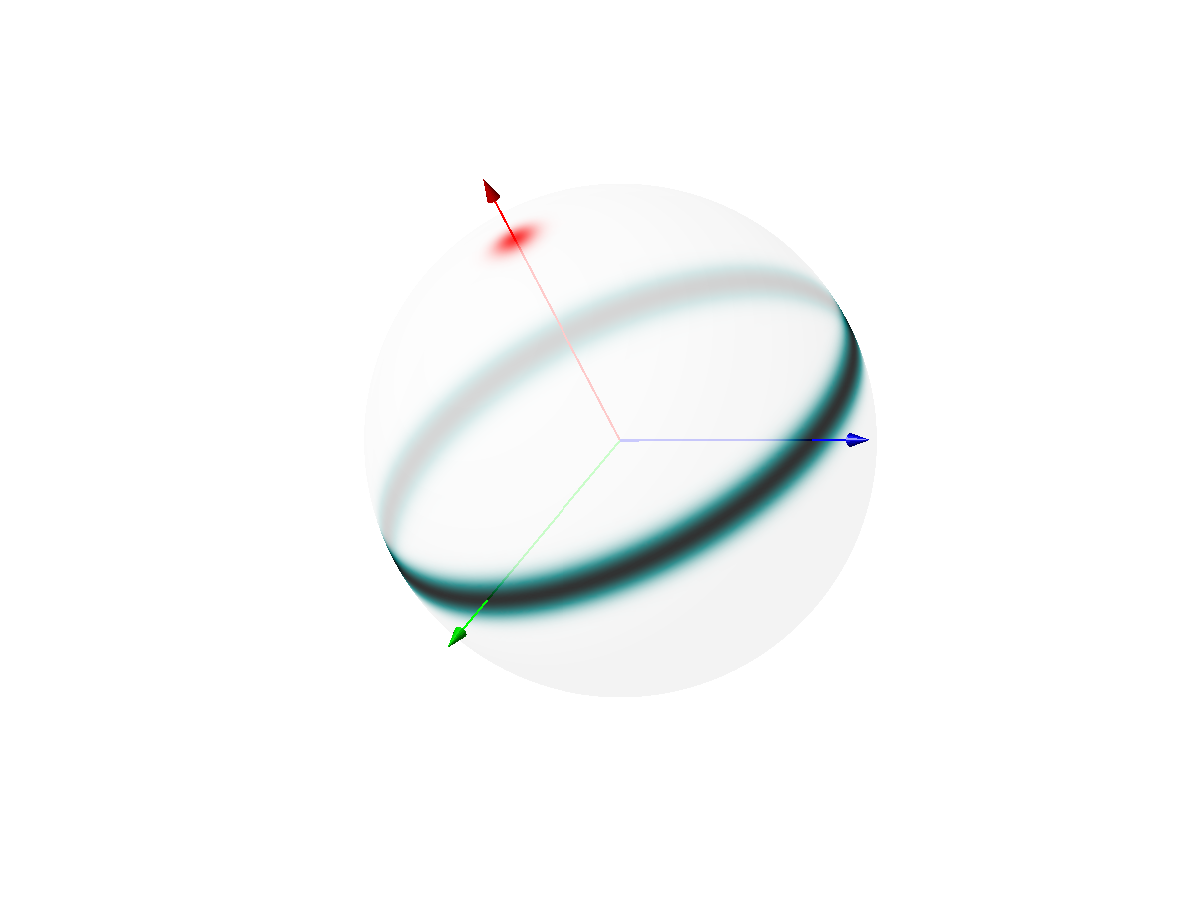
\includegraphics[trim=150 80 120 60, clip, scale=0.45]{figures/observability/est_RI_F5}};
		\node at (7.5,0) {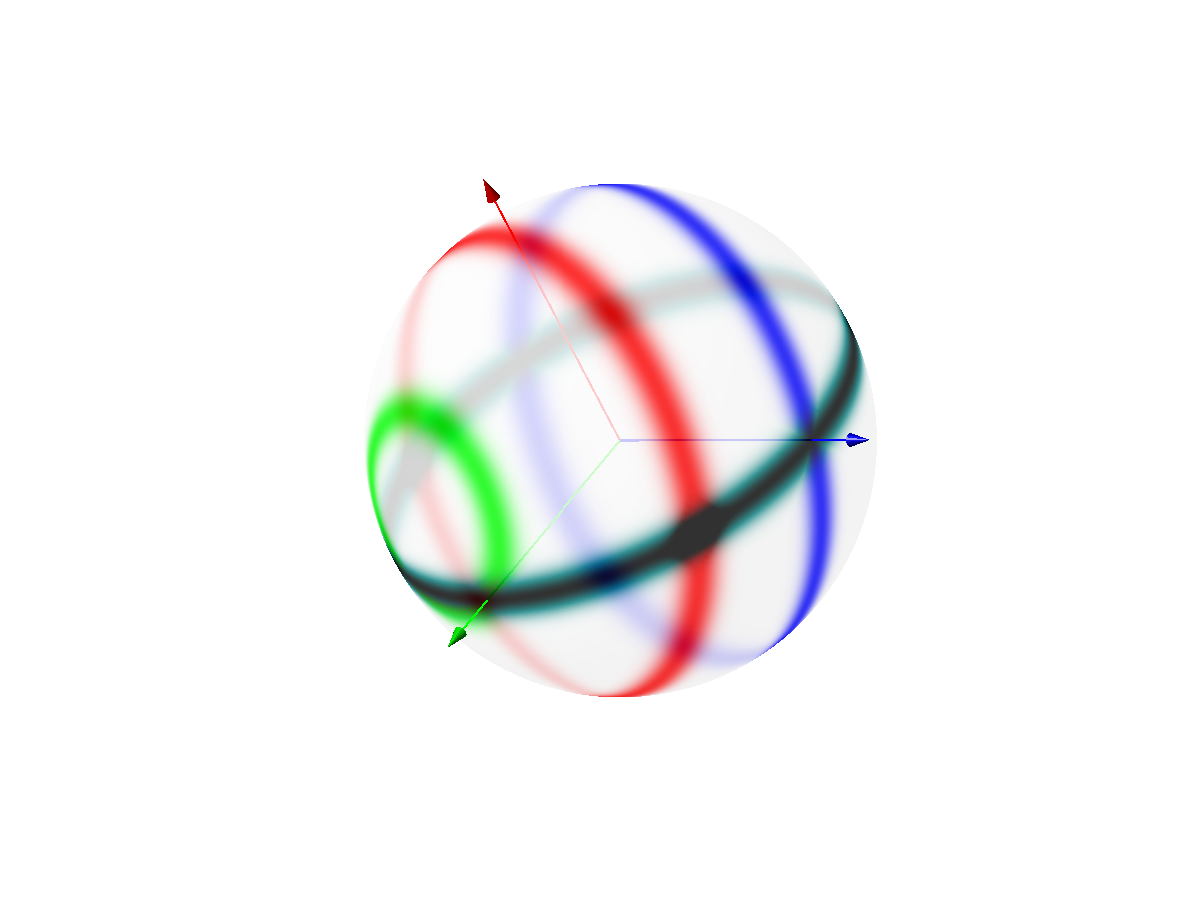
\includegraphics[trim=150 80 120 60, clip, scale=0.45]{figures/observability/est_RI_FN_mea}};
		\node at (12.5,0) {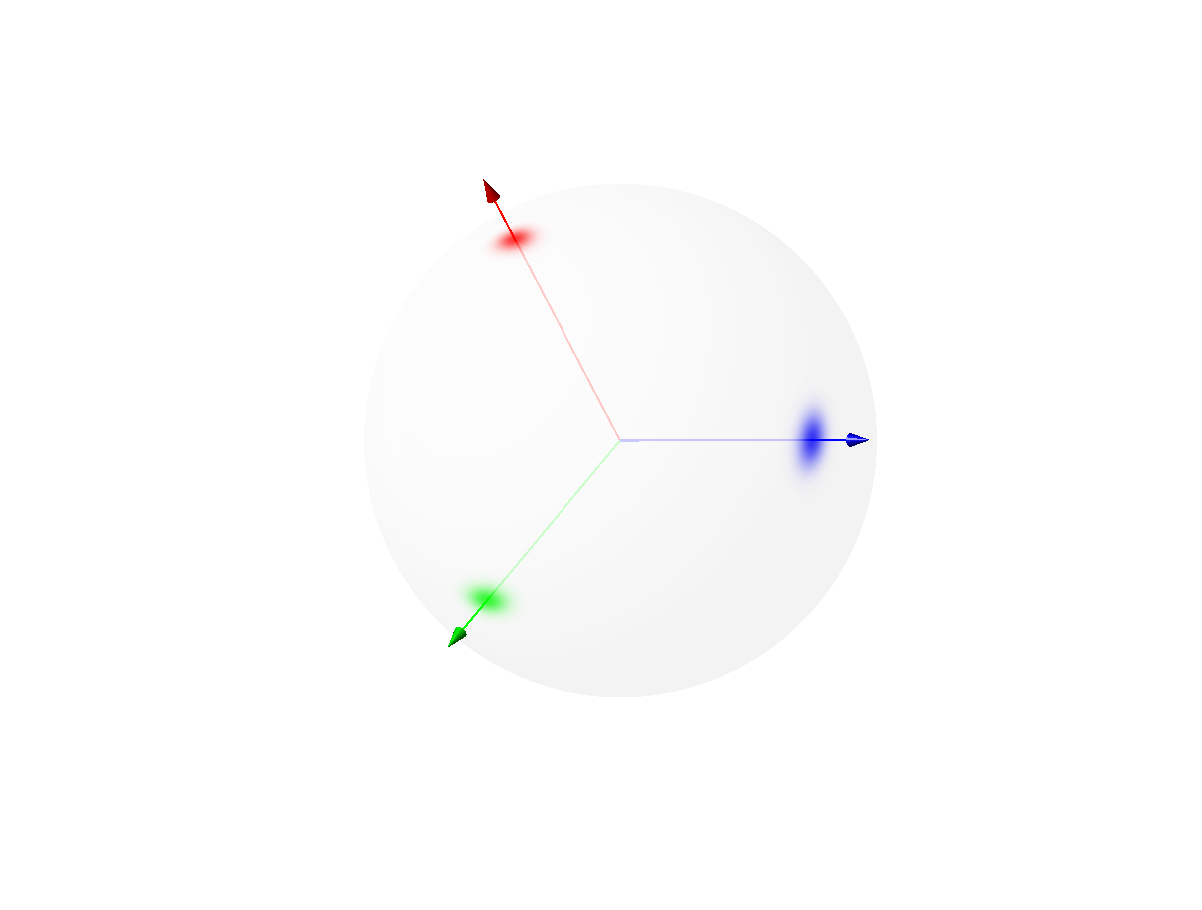
\includegraphics[trim=150 80 120 60, clip, scale=0.45]{figures/observability/est_RI_FN_post}};
		
		\draw[arrows={-Triangle[angle=30:8pt]}] (4.95,3.8) -- ++(90:0.8);
		\draw[arrows={-Triangle[angle=30:8pt]}] (4.95,3.8) -- ++(-30:0.8);
		\draw[arrows={-Triangle[angle=30:8pt]}] (4.95,3.8) -- ++(210:0.8);
		\node at (4.05,3.4) {$\bm{e}_1$};
		\node at (5.95,3.4) {$\bm{e}_2$};
		\node at (4.95,4.8) {$\bm{e}_3$};
		
		\node at (0.5,7.2) {(a)};
		\node at (5.5,7.2) {(b)};
		\node at (10.5,7.2) {(c)};
		\node at (0.5,1.55) {(d)};
		\node at (5.5,1.55) {(e)};
		\node at (10.5,1.55) {(f)};
		
		\node at (2.6,2.6) {Prior dist. at $t=0$};
		\node at (7.7,2.6) {Posterior dist. at $t=0$};
		\node at (12.6,2.6) {Propagated dist. at $t=0.5$};
		
		\node at (2.6,-3.0) {Propagated dist. at $t=1$};
		\node[align=center] at (7.7,-3.0) {Propagated dist. overlapped \\ with measured dist. at $t=1$};
		\node at (12.6,-3.0) {Posterior dist. at $t=1$};
	\end{tikzpicture}
	
	\caption{Estimation with the right trivialized \eqref{eqn:observability-kinematics-right-dist} and the inertial direction measurement \eqref{eqn:observability-measurement-inertial}, where the complete attitude is estimated after incorporating two inertial single direction measurements.}
	\label{fig:observability-est_RI}
\end{figure}

\begin{figure}
	\centering
	\begin{tikzpicture}
		\node at (2.5,5.5) {
\includegraphics[trim=150 80 120 60, clip, scale=0.45]{figures/observability/est_LB_F1_prior}};
		\node at (7.5,5.5) {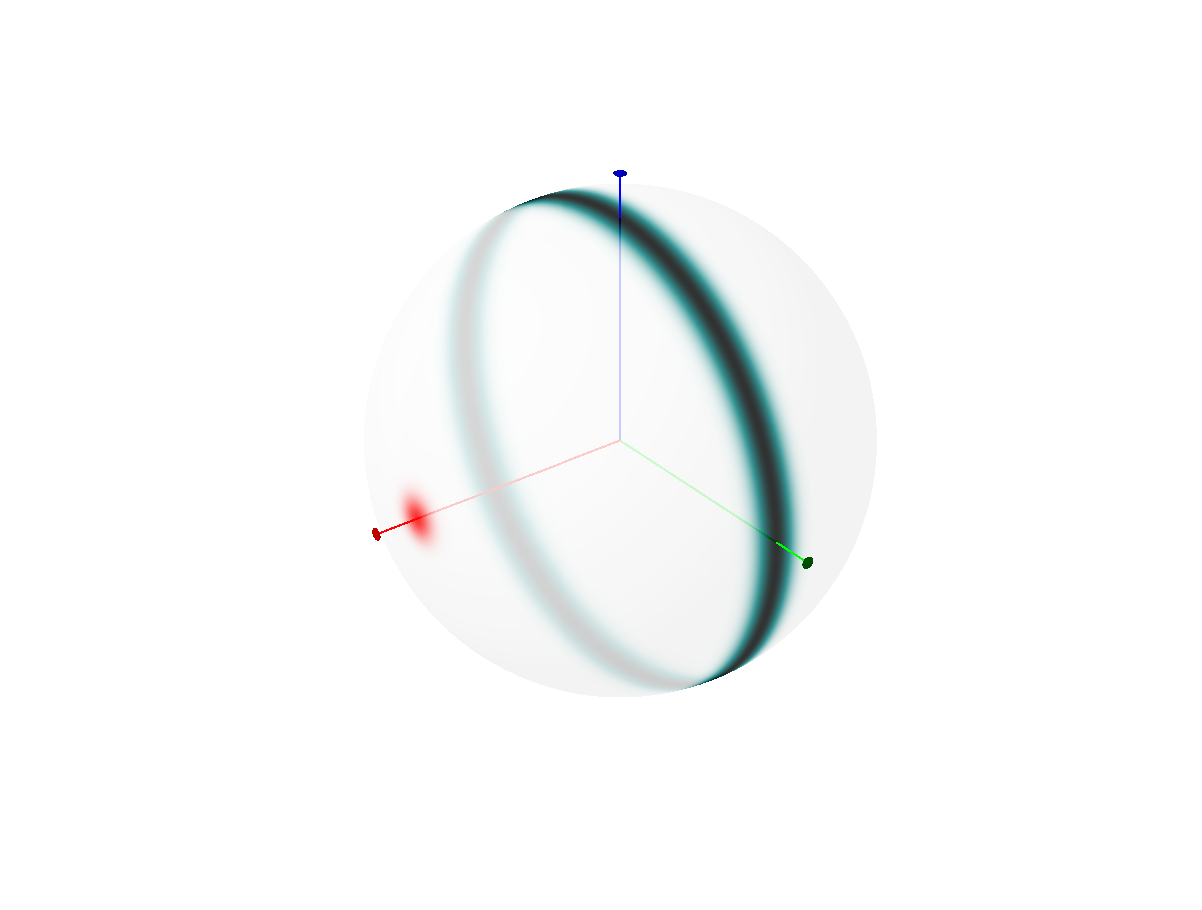
\includegraphics[trim=150 80 120 60, clip, scale=0.45]{figures/observability/est_LB_F1}};
		\node at (12.5,5.5) {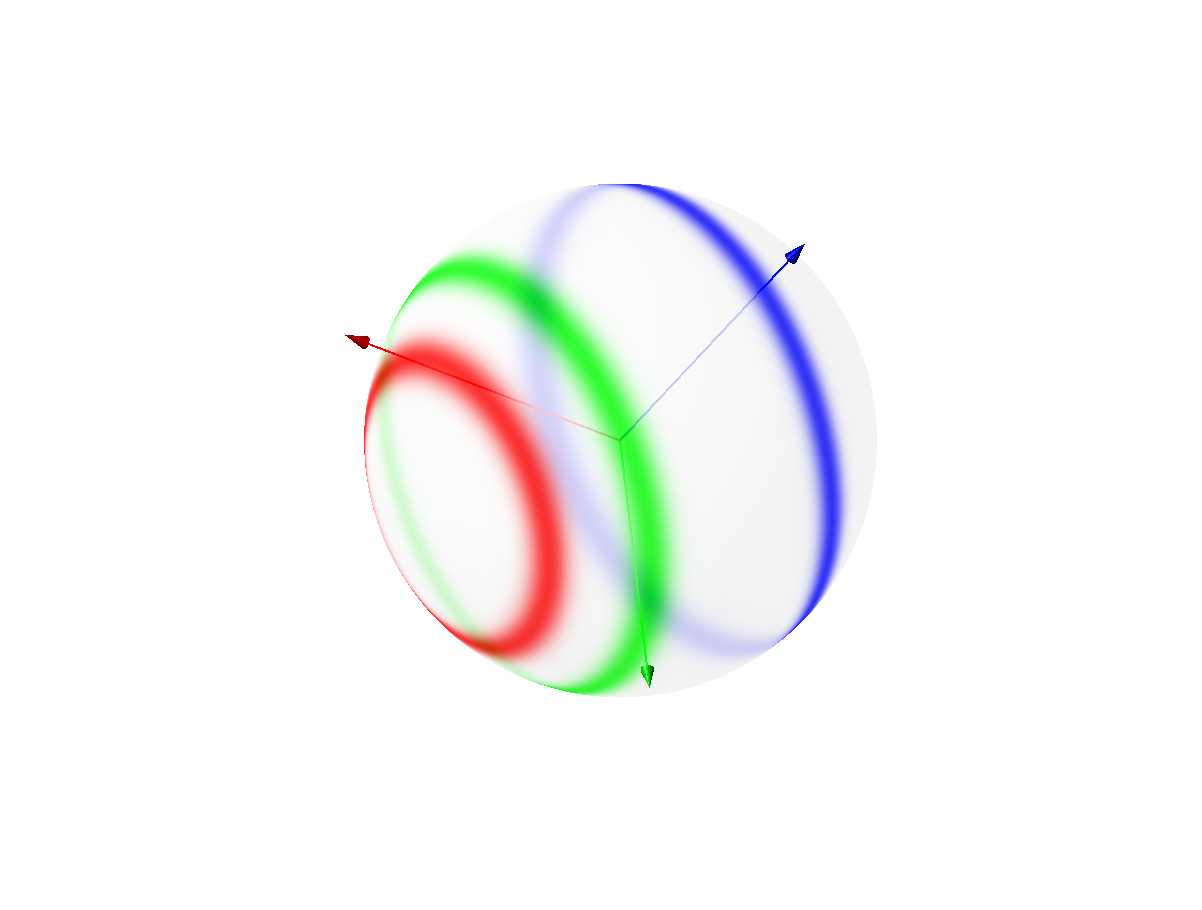
\includegraphics[trim=150 80 120 60, clip, scale=0.45]{figures/observability/est_LB_F3}};
		
		\node at (2.5,0) {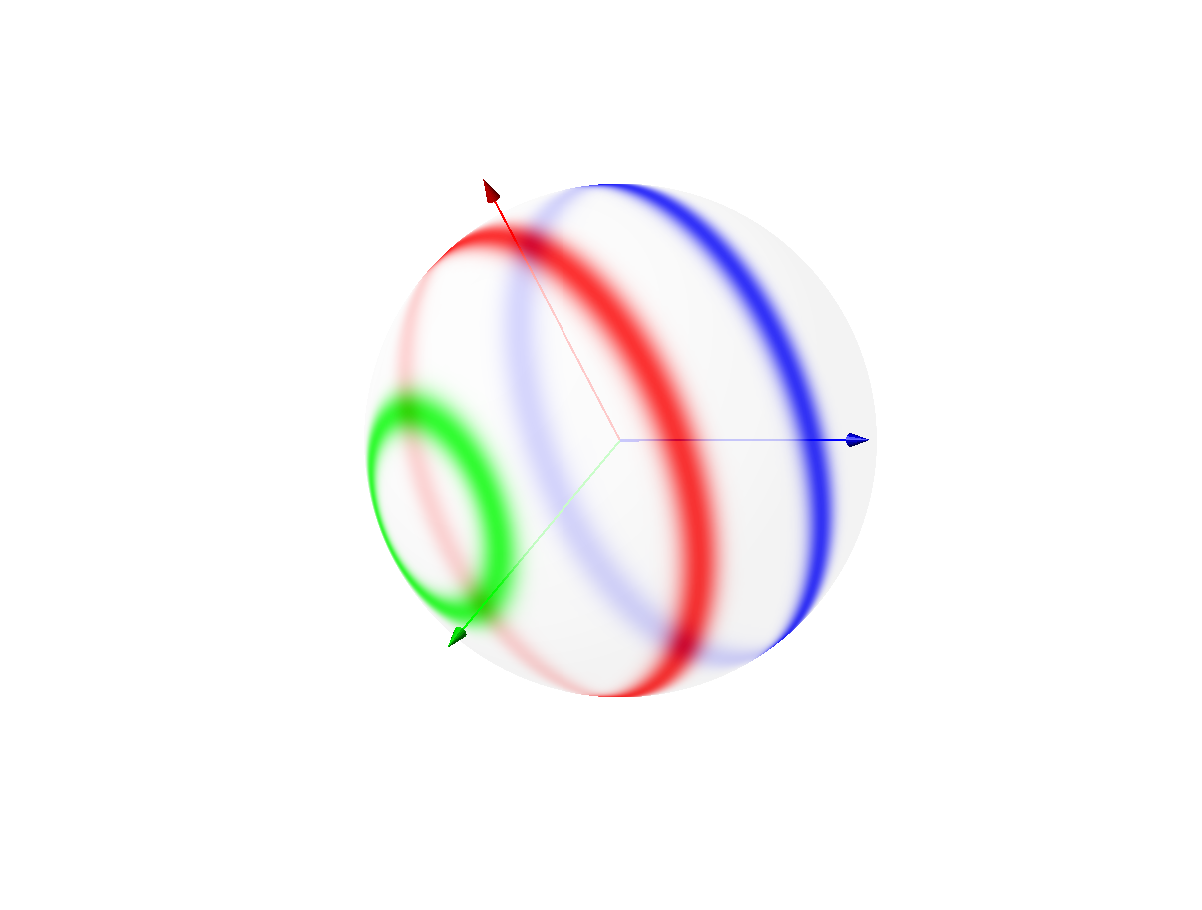
\includegraphics[trim=150 80 120 60, clip, scale=0.45]{figures/observability/est_LB_F5}};
		\node at (7.5,0) {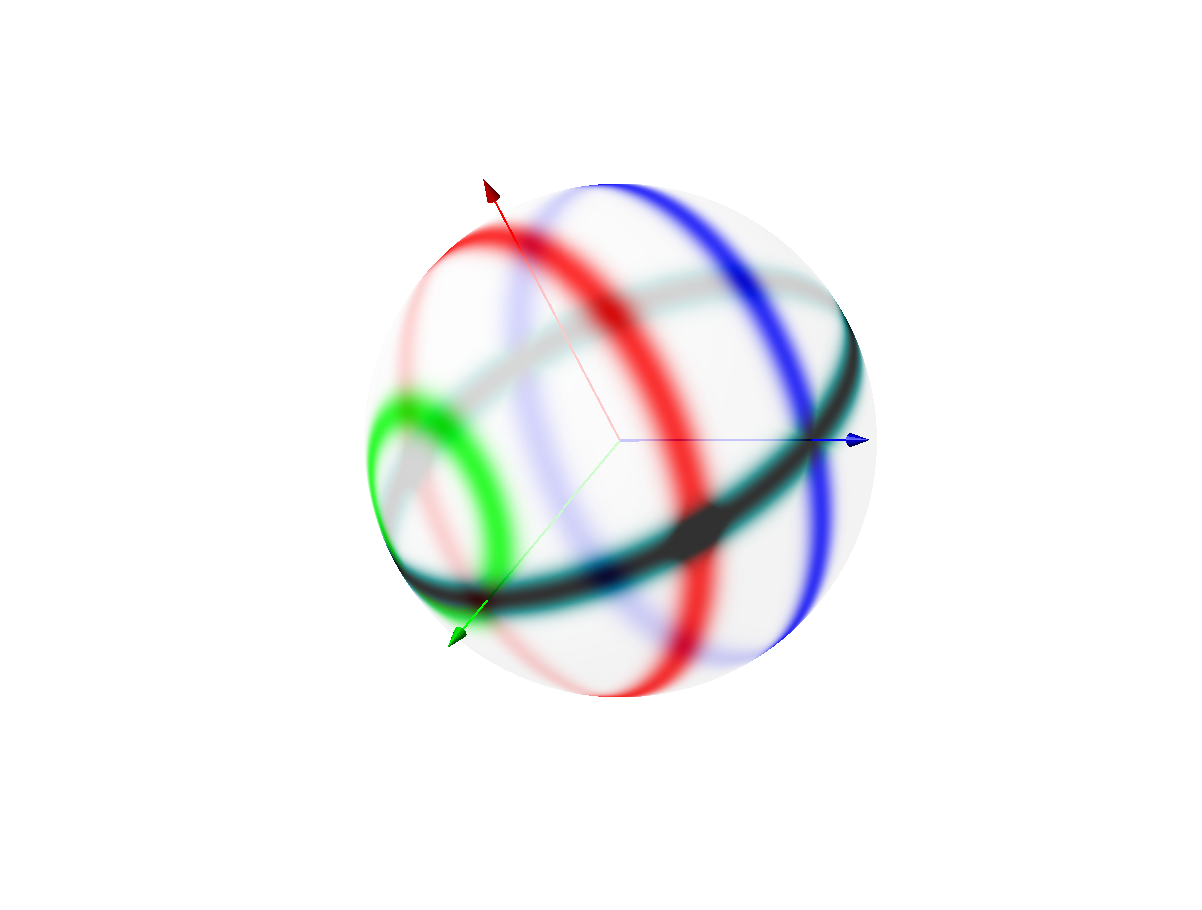
\includegraphics[trim=150 80 120 60, clip, scale=0.45]{figures/observability/est_LB_FN_mea}};
		\node at (12.5,0) {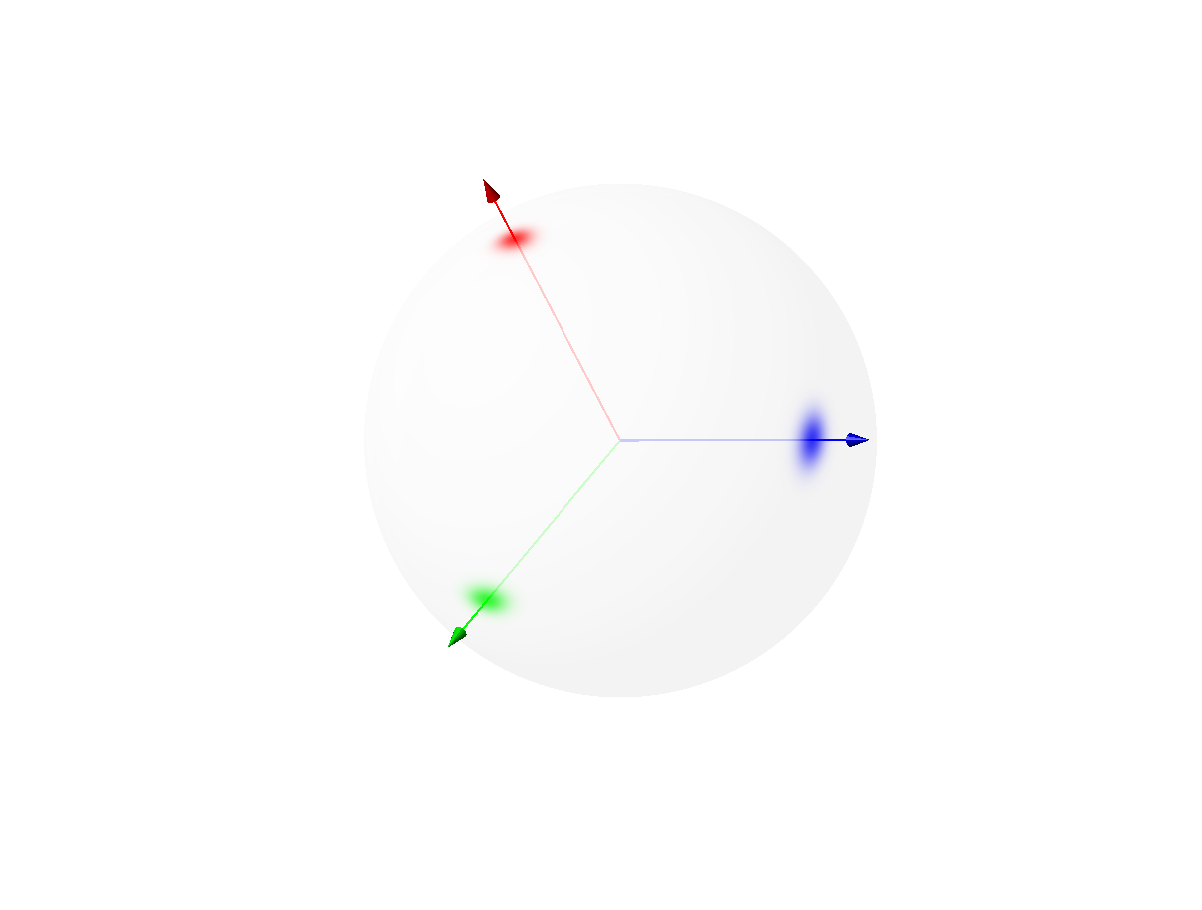
\includegraphics[trim=150 80 120 60, clip, scale=0.45]{figures/observability/est_LB_FN_post}};
		
		\draw[arrows={-Triangle[angle=30:8pt]}] (4.95,3.8) -- ++(90:0.8);
		\draw[arrows={-Triangle[angle=30:8pt]}] (4.95,3.8) -- ++(-30:0.8);
		\draw[arrows={-Triangle[angle=30:8pt]}] (4.95,3.8) -- ++(210:0.8);
		\node at (4.05,3.4) {$\bm{e}_1$};
		\node at (5.95,3.4) {$\bm{e}_2$};
		\node at (4.95,4.8) {$\bm{e}_3$};
		
		\node at (0.5,7.2) {(a)};
		\node at (5.5,7.2) {(b)};
		\node at (10.5,7.2) {(c)};
		\node at (0.5,1.55) {(d)};
		\node at (5.5,1.55) {(e)};
		\node at (10.5,1.55) {(f)};
		
		\node at (2.6,2.6) {Prior dist. at $t=0$};
		\node at (7.7,2.6) {Posterior dist. at $t=0$};
		\node at (12.6,2.6) {Propagated dist. at $t=0.5$};
		
		\node at (2.6,-3.0) {Propagated dist. at $t=1$};
		\node[align=center] at (7.7,-3.0) {Propagated dist. overlapped \\ with measured dist. at $t=1$};
		\node at (12.6,-3.0) {Posterior dist. at $t=1$};
	\end{tikzpicture}

	\caption{Estimation with the left trivialized \eqref{eqn:observability-kinematics-left-dist} and the body-fixed direction measurement \eqref{eqn:observability-measurement-body}, where the complete attitude is estimated after incorporating two body-fixed single direction measurements.}
	\label{fig:observability-est_LB}
\end{figure}

\begin{theorem} \label{thm:observability-obs}
	Consider the two Bayesian attitude estimators for
	\begin{itemize}
		\item right-trivialized angular velocity in the inertial frame  \eqref{eqn:observability-kinematics-right-dist} and inertial direction measurement \eqref{eqn:observability-measurement-inertial} 
		\item left-trivialized angular velocity in the body-fixed frame \eqref{eqn:observability-kinematics-left-dist}, and body-fixed direction measurement \eqref{eqn:observability-measurement-body}  
	\end{itemize}
	with the initial distribution $F_0=0_{3\times 3}$.
	Suppose there is some $k_0$ such that $\omega_{k_0} \times a \neq 0$ for the first case, and $\Omega_{k_0} \times b \neq 0$ for the second case. Then the attitude is observable with probability one for both cases.
\end{theorem}
\begin{proof}
	Consider the first case.
	The posterior distribution after the first measurement is given by $F_1 = \kappa ax_1^T$.
	Suppose $k_0=1$ and denote $\exp(h\hat{\omega}_1) = \delta R$, then by \eqref{eqn:observability-measurement-SVD_FI}, $\eqref{eqn:observability-kinematics-UV_R}$, \eqref{eqn:observability-kinematics-S} and Lemma \ref{lemma:MF-SD}, $U_2^- = \delta R[ a, a', a'' ]$, $S_2^- = \diag\big((s_1)_2^-,0,0\big)$, $V_2^-e_1 = x_1$, where $(s_1)_2^->0$ satisfies
	\begin{align*}
		\frac{1}{c(S_{2}^-)}\frac{\partial c(S_2^-)}{\partial (s_1)_2^-} = (1-h\gamma^2) \frac{1}{c(S_1)}\frac{\partial c(S_1)}{\partial(s_1)_1}.
	\end{align*}
	Thus, the posterior distribution after the second measurement is
	\begin{align} \label{eqn:observability-F2}
		F_2 = (s_1)_2^-\delta Rax_1^T + \kappa ax_2^T.
	\end{align}
	Let $\delta Ra = \alpha a + \alpha'a' + \alpha''a''$ for some $\alpha,\alpha',\alpha''\in\mathbb{R}$. 
	Since $\omega_1\times a\neq 0$, $\alpha'$ and $\alpha''$ cannot both be zeros.
	Then
	\begin{align*}
		F_2 &= (s_1)_2^-(\alpha a + \alpha'a' + \alpha''a'')x_1^T + \kappa ax_2^T \\
		&= a((s_1)_2^-\alpha x_1 + \kappa x_2)^T + (s_1)_2^-\alpha'a'x_1^T + (s_1)_2^-\alpha''a''x_1^T.
	\end{align*}
	Let $v = (s_1)_2^-\alpha_1x_1 + \kappa x_2$, and $v',v''$ be arbitrarily chosen such that $\Big[ \frac{v}{\norm{v}}, v', v'' \Big] \in \SO{3}$.
	Also, let $x_1 = \beta\frac{v}{\norm{v}} + \beta'v' + \beta''v''$. 
	Note that $\beta_2$ and $\beta_3$ cannot both be zeros almost surely.
	Using these, $F_2$ is written as
	\begin{align*}
		F_2 &= \begin{bmatrix}a&a'&a''\end{bmatrix}  \Lambda \begin{bmatrix} \frac{v}{\norm{v}} & v' & v'' \end{bmatrix}^T,
	\end{align*}
	where $\Lambda\in\mathbb{R}^{3\times 3}$ is
	\begin{align*}
		\Lambda = \begin{bmatrix} \norm{v} & 0 & 0 \\ (s_1)_2^-\alpha'\beta & (s_1)_2^-\alpha'\beta' & (s_1)_2^-\alpha'\beta'' \\ (s_1)_2^-\alpha''\beta & (s_1)_2^-\alpha''\beta' & (s_1)_2^-\alpha''\beta'' \end{bmatrix}.
	\end{align*}
	Since $F_2$ is obtained by multiplying rotation matrices to $\Lambda$, it is straightforward to see that $F_2$ and $\Lambda$ share the same proper singular values. 
	Note that $\det(\Lambda) = 0$, so there is at least one zero singular value.
	However, the rank of $\Lambda$ is two almost surely, as at least one element of the right bottom 2-by-2 block is nonzero.
	Thus, $\Lambda$ has only one zero singular value.
	By the definition of proper singular value decomposition, this concludes $\tr{S_2}I_{3\times 3}-S_2$ is positive-definite, and therefore the attitude is observable with probability one.
	
	Next suppose $k_0>1$. By \eqref{eqn:observability-F2}, $F_2 = a((s_2)_1^-x_1+\kappa x_2)^T$ since $\delta R$ does not rotate $a$, which means both the uncertainty propagation and update steps leave $U_ke_1 = a$, $(s_1)_k>0$, and $(s_2)_k=(s_3)_k=0$.
	Thus, the argument in the last paragraph still applies at time $t=t_{k_0}$.
	The proof for the other estimator is similar.
\end{proof}

Finally, it should be noted that although it has been assumed that the attitude follows matrix Fisher distribution, this is not restrictive in the sense that if the initial distribution is uniform, and the angular velocity noise in \eqref{eqn:observability-kinematics-right-dist} and \eqref{eqn:observability-kinematics-left-dist} is zero, i.e., $\gamma=0$, then the attitude conditioned by single direction measurements exactly follows the matrix Fisher distribution.
Therefore, it is supposed that the result presented in Table \ref{table:observability} is not specific to the estimator.
Instead, it is inherent to the observed stochastic dynamical system given by \eqref{eqn:observability-kinematics-right-dist}, \eqref{eqn:observability-kinematics-left-dist} and \eqref{eqn:observability-measurement-inertial}, \eqref{eqn:observability-measurement-body}.
Indeed, it is shown by numerical simulations and experiments that multiplicative extended Kalman filter also exhibits the same observability.
Furthermore, in appendix \ref{app:obervability-deterministic}, it can be proved using classic observability condition that the same observability applies to the deterministic system without noises.

\subsection{Simulations and Experiments}

In this subsection, the attitude observability results presented in Table \ref{table:observability} are validated using numerical simulations and experiments.
The attitude estimation presented in Chapter \ref{section:observability-propagation} and Chapter \ref{section:observability-measurement} based on matrix Fisher distribution, and MEKF are used to estimate the attitude with angular velocity and single directions measurements.

For simulation, a rigid body is assumed to rotate about its third body-fixed axis at \SI{6}{\radian\per\second}, which simultaneously rotates about the second inertial axis at \SI{1}{\radian\per\second}.
The angular velocity is measured at \SI{150}{\hertz} either in the inertial frame or body-fixed frame, with the isotropic random walk noise of $H = \gamma I_{3\times 3}$ where $\gamma = $ \SI{10}{deg/\sqrt{\second}}.
The reference vector is set as $[1,0,0]$, expressed either in the inertial or body-fixed frame, and measured at \SI{30}{\hertz}.
For the matrix Fisher estimator, the measurement noise is formulated as in \eqref{eqn:observability-measurement-inertial} or \eqref{eqn:observability-measurement-body} with $\kappa=200$, 
and the initial attitude distribution is uniform, i.e., $F_0=0_{3\times 3}$.
The noise parameters and initial conditions for MEKF are chosen similarly as the matrix Fisher estimator.

The full attitude error is defined as the angle between the estimated attitude and true attitude.
For the two unobservable combinations, a partial attitude error which neglects the unobserved degree of freedom is also studied.
More specifically, if the reference vector is known in the inertial frame as $a$, then the partial attitude error is defined as $\arccos(R_t^Ta \cdot R^Ta)$, where $R_t$ is the true attitude;
if the reference vector is known in the body-fixed frame as $b$, the partial attitude error is defined as $\arccos(R_tb \cdot Rb)$.
The four combinations of angular velocity and reference vector measurements are labeled as follows:
\begin{center}
	\begin{tabular}{l|cc}
		\diagbox[width=10em]{ref. vec.}{ang. vel.} & body-fixed frame & inertial frame \\ \hline
		body-fixed frame & \textbf{AVB\_RVB} & AVI\_RVB \\
		inertial frame & AVB\_RVI & \textbf{AVI\_RVI}
	\end{tabular}
\end{center}
where the boldface font indicates the cases with observability. 
For each case, 100 Monte Carlo simulations with the simulation period of \SI{60}{\second} are carried out.
The attitude error is first averaged across all timestamps in one simulation, and further averaged across simulations.

\begin{table*}
	\caption{Estimation error (\SI{}{deg}) \label{table:observability-error}}
	\centering
	\begin{tabular}{l|l|c|c|c|c}
		\hline\hline
		\multicolumn{2}{l|}{estimator} & \multicolumn{4}{c}{matrix Fisher} \\ \hline
		\multicolumn{2}{l|}{case (\textbf{observable}, unobservable)} & \textbf{AVI\_RVI} & AVI\_RVB & AVB\_RVI & \textbf{AVB\_RVB} \\ \hline
		\multirow{2}{*}{simulation} & full error $\pm$ s.d. & 6.57$\pm$0.25 & 90$\pm$0 & 90$\pm$0 & 5.71$\pm$0.15  \\
		& partial error $\pm$ s.d. & - & 3.33$\pm$0.06 & 3.34$\pm$0.06 & - \\ \hline
		\multirow{2}{*}{experiment} & full error & 7.15 & 90.29 & 90.41 & 1.74 \\
		& partial error & - & 0.63 & 3.02 & - \\ \hline\hline
		\multicolumn{2}{l|}{estimator} & \multicolumn{4}{c}{MEKF} \\ \hline
		\multicolumn{2}{l|}{case (\textbf{observable}, unobservable)} & \textbf{AVI\_RVI} & AVI\_RVB & AVB\_RVI & \textbf{AVB\_RVB} \\ \hline
		\multirow{2}{*}{simulation} & full error $\pm$ s.d. & 7.02$\pm$0.50 & 135$\pm$24 & 89$\pm$37 & 6.06$\pm$0.27 \\
		& partial error $\pm$ s.d. & - & 3.33$\pm$0.06 & 3.33$\pm$0.06 & - \\ \hline
		\multirow{2}{*}{experiment} & full error & 15.92 & 161.21 & 93.32 & 18.94 \\
		& partial error  & - & 2.95 & 6.43 & - \\ \hline\hline
	\end{tabular}
\end{table*}

The attitude estimation errors are summarized in Table \ref{table:observability-error}.
It is clearly shown that for the two observable cases (AVI\_RVI and AVB\_RVB), the full attitude can be estimated with the average error of about \SI{6}{\degree}.
On the other hand, for the two unobservable cases (AVI\_RVB and AVB\_RVI), the full attitude error is around \SI{90}{\degree}, and the partial attitude error is around \SI{3.3}{\degree}.
For a more straightforward comparison, the time evolution of attitude errors for a single simulation is shown in Figure \ref{fig:observability-attitudeError}, where it is illustrated that for the two observable cases, the full attitude error quickly converges from \SI{180}{\degree} to around zero;
whereas for the two unobservable cases, the full attitude error never converges, but the partial attitude error remains low throughout the simulation since the initial partial error is zero.

The attitude observability is also indicated by the estimated dispersion, quantified as the standard deviation of the error rotation vector as shown in Figure \ref{fig:observability-attitudeStd}.
For the two observable cases, the standard deviations along all three axes remain below \SI{10}{\degree}, with the rotation about the reference vector (the first axis $e_1$) a little bit larger than the two other axes.
For the two unobservable cases, the standard deviation along the reference vector for the matrix Fisher estimator is mostly above $10^7$ \SI{}{deg}, which  indicates a uniform distribution.
For the MEKF, if the reference vector is known in the body-fixed frame, the standard deviation along the reference vector is similar to the matrix Fisher estimator, which is above $10^6$ \SI{}{deg}.
However, if the reference vector is known in the inertial frame, the standard deviation is around \SI{15}{\degree}, which is only marginally larger than the observable cases.
This discrepancy is caused by that the error rotation vector is expressed in the body-fixed frame, rather than in the inertial frame.
And if the reference vector is known in the inertial frame, MEKF has been shown to apply some slight but erroneous corrections to the rotation about the reference vector due to the linearization of the measurement function~\cite{li2012improving}.

\begin{figure}
	\centering
	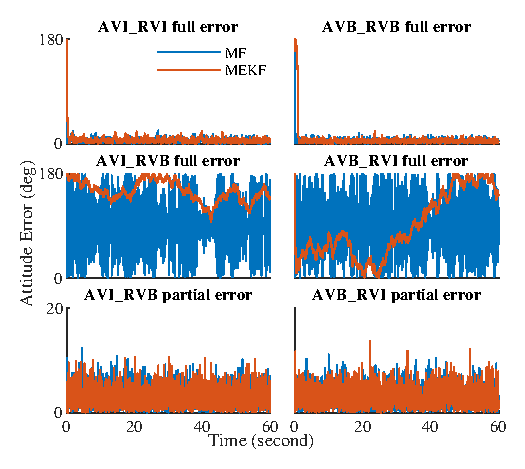
\includegraphics[scale=1.4]{figures/observability/attitudeError}
	\caption{Attitude errors for the matrix Fisher (MF) estimator and MEKF in four combinations of angular velocity and reference vector measurements. \label{fig:observability-attitudeError}}
\end{figure}

\begin{figure}
	\centering
	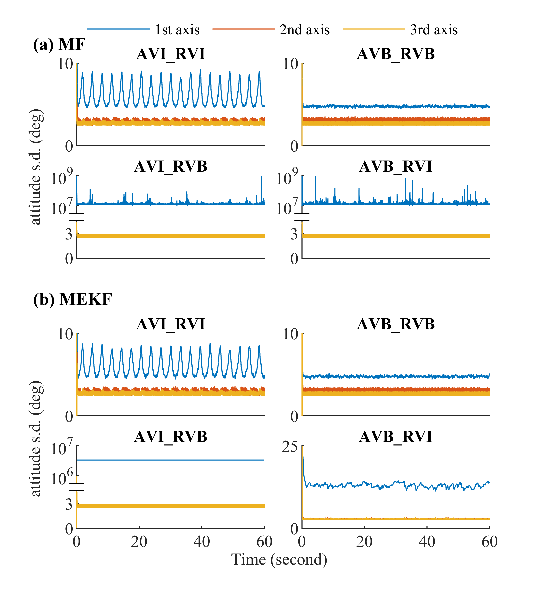
\includegraphics[scale=1.4]{figures/observability/attitudeStd}
	\caption{Attitude standard deviations for the matrix Fisher (MF) estimator and MEKF.
		In the ``RVI'' and ``RVB'' cases, the attitude covariance matrix is expressed in the inertial and body-fixed frames respectively.
		For the MF filter, $(\tr{S}I_{3\times 3}-S)^{-1}$ is used as the attitude covariance matrix in the principal axes frame. \label{fig:observability-attitudeStd}}
\end{figure}

\begin{figure}
	\begin{subfigure}{0.45\textwidth}
		\centering
		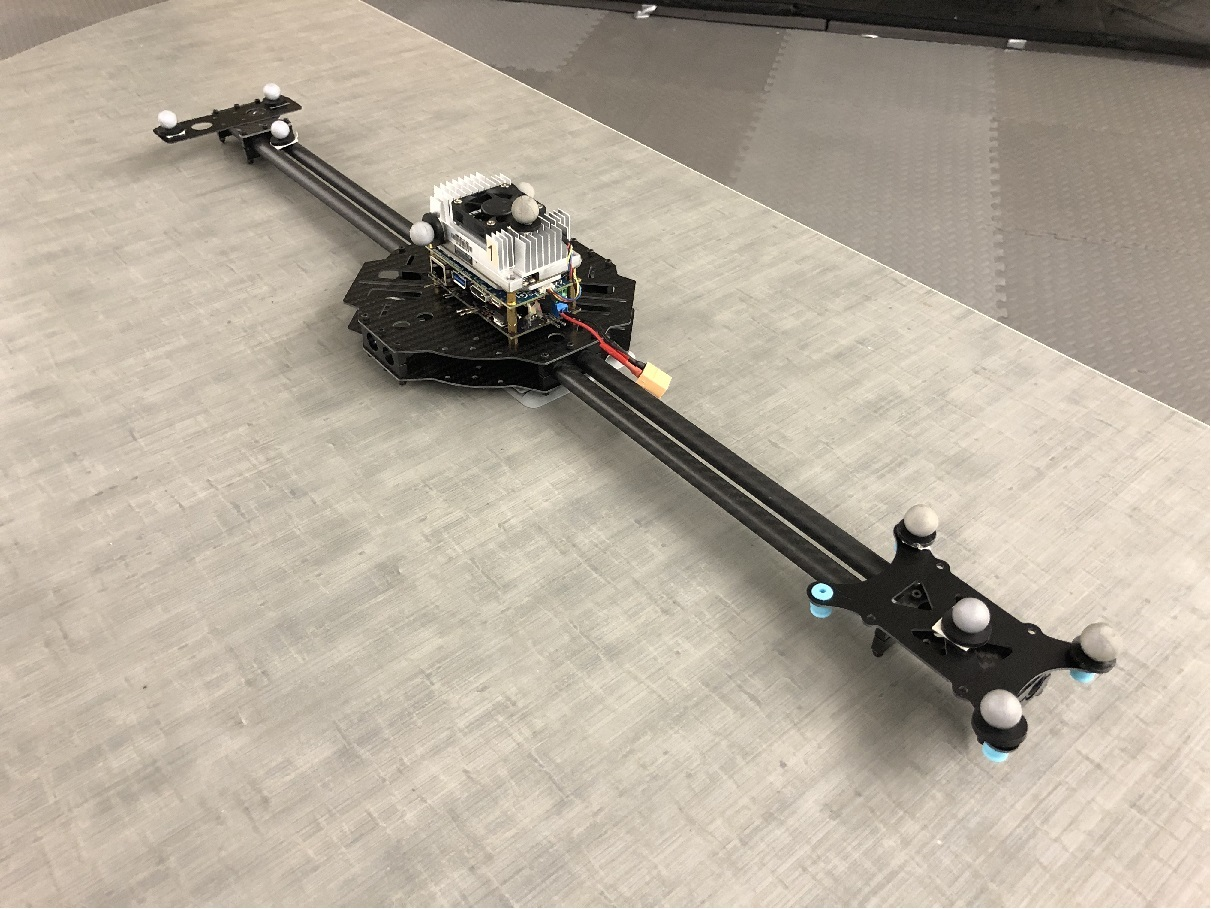
\includegraphics[width=\textwidth]{figures/observability/exp1.jpeg}
		\caption{Hardware configuration with reflective markers for a VICON motion capture system}
	\end{subfigure}
	\hspace{0.1\textwidth}
	\begin{subfigure}{0.45\textwidth}
		\centering
		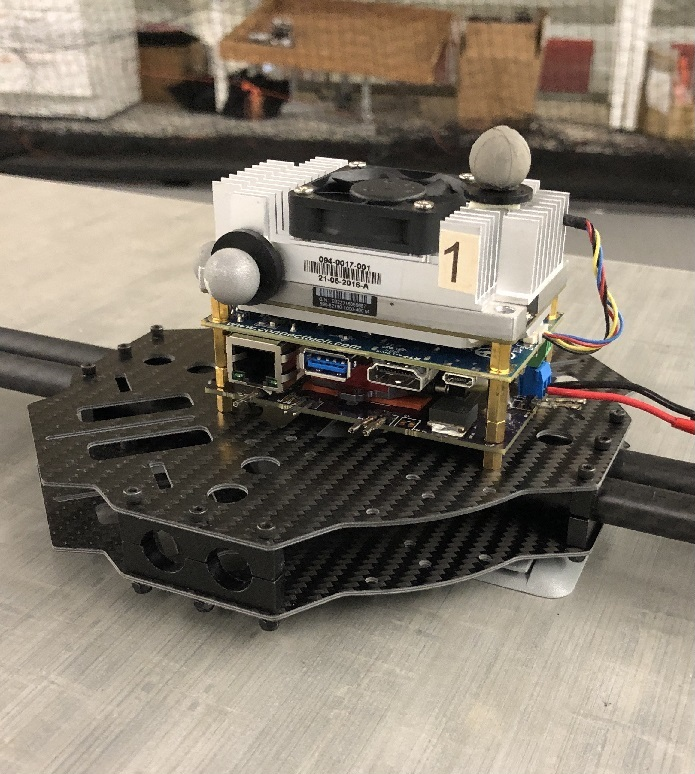
\includegraphics[width=\textwidth]{figures/observability/exp2.jpeg}
		\caption{Onboard computing module connected to IMU through a custom-made printed circuit board}
	\end{subfigure}
	\caption{Hardware platform for experiments} \label{fig:observability-exp-hardware}
\end{figure}

The attitude observability was also validated through experiments.
We use a custom-made hardware platform (Figure \ref{fig:observability-exp-hardware}), which has been developed for autonomous unmanned aerial vehicles, to collect measurements while moving it with hands.
An external VICON motion capture system detects reflective markers attached to the platform to determine its attitude, which is used as the ground truth attitude.
A 9-axis inertial measurement unit (VectorNav VN100) is attached to the platform, and the onboard gyroscope provides the angular velocity measurement in the body-fixed frame, which is also converted into the angular velocity measurement in the inertial frame using the ground truth attitude. 
For the inertial direction measurement, the direction of gravity is measured by the accelerometer in IMU.
Moreover, for the body-fixed direction measurement, two additional markers are attached to the platform as a known and fixed reference vector in the body-fixed frame, which is measured by the Vicon motion system in the inertial frame.
All Vicon and IMU measurements are synchronized and sampled at \SI{100}{\hertz}, using an onboard Nvidia Jetson TX2 computing module.
The platform was rotated around its roll, pitch and yaw axes during the data collection.
The matrix Fisher estimator and MEKF are run off-board using the collected experimental data, with the single vector measurement update applied at \SI{20}{\hertz}.
The noise parameters and initial conditions are set the same as in the simulation.
Note that these are not carefully tuned for the specific hardware, since the main objective is to verify the observability.

\begin{figure}
	\centering
	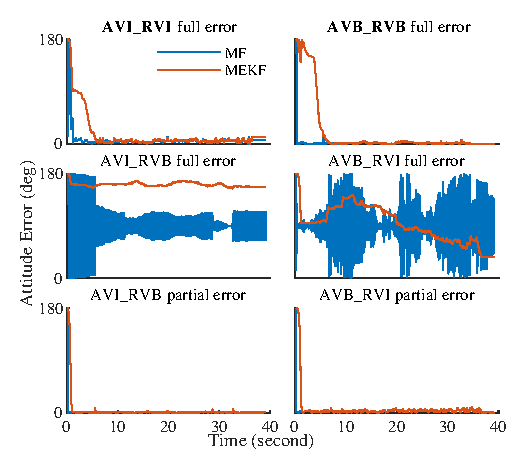
\includegraphics[scale=1.4]{figures/observability/attitudeError-Exp}
	\caption{Attitude errors for the matrix Fisher estimator (MF) and MEKF. \label{fig:observability-attitudeError-Exp}}
\end{figure}

\begin{figure}
	\centering
	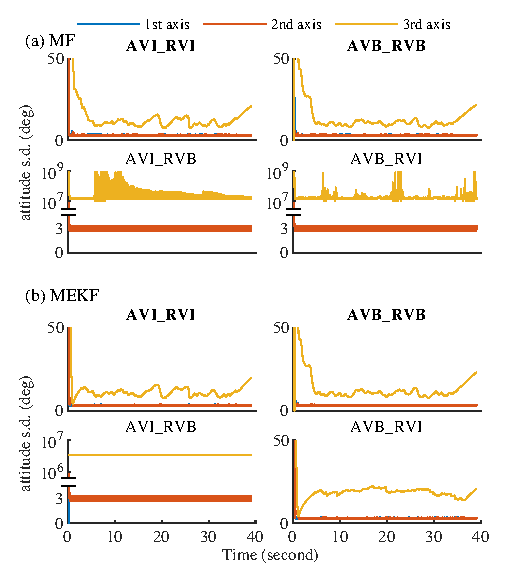
\includegraphics[scale=1.4]{figures/observability/attitudeStd-Exp}
	\caption{Attitude uncertainty for the matrix Fisher estimator (MF) and MEKF.
		In the ``RVI'' cases, the attitude covariance matrix is expressed in the inertial frame; and in the ``RVB'' cases, it is expressed in the $b'$-$b''$-$b$ frame, where $b$ is the reference vector when resolved in the body-fixed frame, and $b',b''$ are perpendicular to $b$.
		For the MF filter, $(\tr{S}I_{3\times 3}-S)^{-1}$ is used as the attitude covariance matrix in the principal axes frame. \label{fig:observability-attitudeStd-Exp}}
\end{figure}

The attitude errors for the four combinations of measurements are presented in Figure \ref{table:observability-error} and Figure \ref{fig:observability-attitudeError-Exp}.
Similar with the simulation results, for the two observable cases (AVI\_RVI and AVB\_RVB) the full attitude error converges to around zero within \SI{10}{\second}; whereas for the two unobservable cases (AVI\_RVB and AVB\_RVI) only the partial error converges.
The standard deviation of the rotation vector is demonstrated in Figure \ref{fig:observability-attitudeStd-Exp}.
Again the uncertainties for the two observable cases are small in all three axes, but those for the two unobservable cases are only small in two axes, which is very similar to the simulation results.

\section{Attitude Estimation}

In the previous section, a Bayesian attitude estimator is proposed to estimate the attitude with a gyroscope and repeated measurements of a single reference direction, in order to study attitude observability.
In \eqref{eqn:observability-kinematics-left}, it is assumed that the angular velocity measured from a gyroscope is affected by a white noise.
However, usually the gyroscope noise also contains a random walk term, referred to as the bias \cite{crassidis2007survey}.
As a random walk process, the gyroscope bias is time varying, and can easily deteriorate the integrated attitude in short time if it is not properly compensated for.
Therefore, an attitude estimator also needs to estimate the bias, simultaneously with the attitude.

Concurrent estimation of attitude and gyroscope bias has been studied in numerous works, as reviewed in Chapter \ref{section:intro-review-estimation}.
Nevertheless, most existing algorithms rely on variations of Kalman filter, which uses Gaussian distribution to model attitude dispersion, thus they cannot handle large attitude uncertainty as shown in Figure \ref{fig:wrapping}.
Although the matrix Fisher and Bingham distributions have been applied to deal with large uncertainty \cite{glover2014tracking,kurz2014recursive,lee2018bayesian}, they cannot estimate the gyroscope bias as the two distributions cannot model the correlation between attitude and gyroscope bias.

The introduction of matrix Fisher--Gaussian distribution in Chapter \ref{chap:MFG} was primarily motivated to use matrix Fisher distribution to deal with large attitude uncertainty, while estimating the gyroscope bias.
The correlation between attitude and bias is directly handled by the MFG in a global and singularity free fashion, allowing the attitude uncertainty to be very large.
In this section, a new recursive Bayesian attitude estimator is proposed based on MFG to estimate the attitude and gyroscope bias concurrently.

\subsection{Problem Formulation} \label{section:attEst-problem}

In this section, the following gyroscope kinematics is considered:
\begin{gather}
	R^T\diff{R} = (\hat{x}+\hat{\Omega})\diff{t} + (H_udW_u)^\wedge, \label{eqn:attEst-kinematics-att} \\
	\diff{x} = H_vdW_v \label{eqn:attEst-kinematics-bias},
\end{gather}
where $R\in\SO{3}$ is the attitude of a rigid body and $x\in\mathbb{R}^3$ is the bias of the onboard gyroscope.
The vector $\Omega\in\mathbb{R}^3$ is the angular velocity measured by the gyroscope that is resolved in the body-fixed frame.
Next, $W_u$ and $W_v\in\mathbb{R}^3$ are two independent three-dimensional Wiener processes, and $H_u, H_v \in \mathbb{R}^{3\times 3}$ are two matrices describing the strengths of noises.
The angular velocity measurement has two sources of noises: the bias term $x$ and the Gaussian white noise contributed by $H_u dW_u$.
The bias is slowly varying while being driven by another white noise $H_v dW_v$.

The stochastic differential equation \eqref{eqn:attEst-kinematics-att} is interpreted in the Stratonovich sense to guarantee the process does not leave $\SO{3}$ \cite{barrau2018stochastic,markley2006attitude}.
Let the time be discretized by a sequence $\{t_0,t_1,\ldots\}$. 
For convenience, it is assumed that the time step $h\in\mathbb{R}$ is fixed, i.e., $h= t_{k+1} - t_k$ for any $k$. 
According to \cite[Eqn. 14]{barrau2018stochastic}, the kinematics model can be discretized into
\begin{gather}
	R_{k+1} = R_k \exp\left\{ h (\hat{\Omega}_k+\hat{x}_k) + (H_u\Delta W_u)^\wedge \right\}, \label{eqn:attEst-kinematics-att-dist} \\
	x_{k+1} = x_k + H_v\Delta W_v,  \label{eqn:attEst-kinematics-bias-dist}
\end{gather}
where $\Delta W_u, \Delta W_v\in\mathbb{R}^{3\times 3}$ are the stochastic increments of the Wiener processes over a time step, which are Gaussian with
\begin{equation}\label{eqn:attEst-kinematics-DeltaW}
	H_u\Delta W_u \sim \mathcal{N}(0,hG_u), \quad H_v\Delta W_v \sim \mathcal{N}(0,hG_v),
\end{equation}
where $G_u = H_uH_u^T$ and $G_v = H_vH_v^T\in\mathbb{R}^{3\times 3}$.

Two types of measurements are considered available at $t_k$, $k\geq 1$: (i) when the attitude is directly measured, and (ii) when reference directions in the inertial frame, such as the direction of magnetic field or gravity, are measured.
First, suppose the attitude is measured by $N_a$ attitude sensors as $Z_i\in\SO{3}$, whose error is distributed by the matrix Fisher distribution.
More specifically, given the true attitude $R_t\in\SO{3}$, the measurement error $R_t^TZ_i\in\SO{3}$ follows the matrix Fisher distribution with the parameter $F_{Z_i}\in\mathbb{R}^{3\times 3}$ for $i=1,\ldots, N_a$, which characterizes the accuracy and bias of the $i$-th attitude sensor. 

Next, suppose there are also $N_v$ fixed reference vectors ${a}_j\in\mathbb{S}^2$ in the inertial reference frame, which are measured by direction sensors in the body-fixed frame as ${z}_j\in\mathbb{S}^2$ for $j=1,\ldots,N_v$.
Furthermore, given the true attitude $R_t$, the noisy measurement ${z}_j$ is assumed to follow the von Mises Fisher distribution \cite{mardia2009directional} with mean direction $R_t^TB_j{a}_j\in\mathbb{S}^2$ and concentration parameter $\kappa_j>0$.
The parameter $B_j\in\SO{3}$ specifies the constant bias of the direction sensor, and $\kappa_j$ specifies the concentration of its random noise.
The measurements $\Big\{\{Z_i\}_{i=1}^{N_a}, \{z_j\}_{j=1}^{N_v}\Big\}$ at time $t_k$ are altogether denoted by $\mathcal{Z}_k$.

The initial attitude and bias $(R_0,x_0)$ at $t_0$ are assumed to follow MFG with $n=3$ and $(\mu_0, \Sigma_0, P_0, U_0, S_0, V_0)$ of appropriate dimensions.
Given the gyroscope measurements $\{\Omega_k\}_{k=0}^\infty$, and the attitude and direction measurements $\{\mathcal{Z}_k\}_{k=1}^\infty$ at discrete time instants, the problem is to find the posterior distribution of $(R_k,x_k) | \{\mathcal{Z}_m\}_{m=1}^k$, and approximate it to an MFG with parameters $(\mu_k, \Sigma_k, P_k, U_k, S_k, V_k)$.
To find the posterior distribution, two steps are needed: first the uncertainty is propagated from $(R_k,x_k) | \{\mathcal{Z}_m\}_{m=1}^k$ to $(R_{k+1},x_{k+1}) | \{\mathcal{Z}_m\}_{m=1}^k$ according to the gyroscope kinematics equations \eqref{eqn:attEst-kinematics-att-dist} and \eqref{eqn:attEst-kinematics-bias-dist}.
Second, the prior distribution $(R_{k+1},x_{k+1}) | \{\mathcal{Z}_m\}_{m=1}^k$ is updated by the measurements $\mathcal{Z}_k$ using Bayes's formula into $(R_{k+1},x_{k+1}) | \{\mathcal{Z}_m\}_{m=1}^{k+1}$.
These two steps are developed using the MFG in the next two subsections.

\subsection{Uncertainty Propagation} \label{section:attEst-propagation}

Suppose $(R_k,x_k) | \{\mathcal{Z}_m\}_{m=1}^k \sim\mathcal{MG}(\mu_k, \Sigma_k, P_k, U_k, S_k, V_k)$. 
In this subsection, the expectations of $(R_{k+1},x_{k+1})$ used in the MLE of MFG are calculated to construct a new MFG describing the uncertainty of $(R_{k+1},x_{k+1})$.
The expectations are calculated in two different ways: (i) approximate analytical expressions are developed directly from the gyroscope kinematics, and (ii) they are approximated empirically using deterministically sampled sigma points.

Let us first look at how to develop analytical expressions for required moments.
The exponent in \eqref{eqn:attEst-kinematics-att-dist} can be decomposed into
\begin{align*}
	\{h(\Omega_k + \mu_k)\} + \{h(x_k-\mu_k) + H_u \Delta W_u\},
\end{align*}
after taking the hat map off. 
The first part is deterministic, and the second part is a random vector with zero mean.  
This leads to the following approximation to \eqref{eqn:attEst-kinematics-att-dist}.

\begin{lemma}
	Equation \eqref{eqn:attEst-kinematics-att-dist} is almost surely equivalent to
	\begin{align} \label{eqn:attEst-kinematics-att-factorization}
		R_{k+1} = & R_ke^{h(\hat{x}_k-\hat{\mu}_k) + (H_u\Delta W_u)^\wedge + o(h)} e^{h(\hat{\Omega}_k+\hat{\mu}_k)}.
	\end{align}
\end{lemma}
\begin{proof}
	Equation \eqref{eqn:attEst-kinematics-att-dist} is rewritten into 
	\begin{align*} 
		R_{k+1} &= R_k \left[ e^{h(\hat{\Omega}_k+\hat{x}_k) + (H_u\Delta W_u)^\wedge} 
		e^{-h(\hat{\Omega}_k+\hat{\mu}_k)} \right] e^{h(\hat{\Omega}_k+\hat{\mu}_k)}.
	\end{align*}
	The Baker-Campbell-Hausdorff (BCH) formula provides the solution of $Z$ to the equation $e^X e^Y = e^Z$ for given $X,Y$. 
	Applying this to the expression in the square brackets,  
	\begin{align} \label{eqn:attEst-kinematics-att-factorization-proof}
		R_{k+1} &= R_k e^{h(\hat{x}_k-\hat{\mu}_k) + (H_u\Delta W_u)^\wedge + A} e^{h(\hat{\Omega}_k+\hat{\mu}_k)},
	\end{align}
	where the additional term $A\in\so{3}$ is composed of at least twice iterated Lie brackets, and it is of the order of $h^2$ and $h\Delta W_u$.
	Since $\lim\limits_{h \to 0}\Delta W_u=0$ almost surely, $A \sim o(h)$.
\end{proof}

This lemma is helpful in making use of the closed form expression of the exponential map \eqref{eqn:rv2rot} for the deterministic components of \eqref{eqn:attEst-kinematics-att-dist}.
The uncertainty of $R_{k+1}$ contributed by the noises is quantified by the centered stochastic component $h(x_k-\mu_k) + H_u\Delta W_u$ with zero mean.
Next, an expression for $\expect{R_{k+1}}$ is derived to solve the marginal MLE.

\begin{theorem} \label{thm:attEst-prop-E(R_{k+1})}
	The expectation of the propagated attitude $R_{k+1}$ is given by
	\begin{align} \label{eqn:attEst-prop-E(R_{k+1})}
		\expect{R_{k+1}} = \left\{ \expect{R_k}\left( I_{3\times 3} + \tfrac{h}{2}(G_u-\tr{G_u}I_{3\times 3}) \right) + hU_k\expect{Q_kV_k^T\widehat{P_k\nu_{R_k}}} \right\} e^{h(\hat{\Omega}_k+\hat{\mu}_k)} + O(h^2),
	\end{align}
	where $Q_k=U_k^TR_kV_k$, $\nu_{R_k} = (Q_kS_k-S_kQ_k^T)^\vee$ for MFGI, or $\nu_{R_k} = (S_kQ_k-Q_k^TS_k)^\vee$ for MFGB.
\end{theorem}
\begin{proof}
	First, expand the first exponential term in \eqref{eqn:attEst-kinematics-att-factorization} into an infinite sum as
	\begin{align}
		e^{h (\hat x_k-\hat{\mu}_k) + (H_u\Delta W_u)^\wedge + o(h)} = \sum_{i=0}^\infty \tfrac{1}{i!}\left\{ h (\hat x_k-\hat{\mu}_k) + (H_u\Delta W_u)^\wedge + o(h) \right\}^i.
	\end{align}
	Note that (i) $\Delta W_u$ is a zero mean Gaussian vector with covariance matrix $hI_{3\times3}$, so its odd order moments are zero, and $\expect{\left((H_u\Delta W_u)^\wedge\right)^{2n}} \sim O(h^n)$; (ii) $o(h)$ in the above equation only has terms of order at least $h^2$ or $h\Delta W_u$ as shown in \eqref{eqn:attEst-kinematics-att-factorization-proof}.
	Combining these two observations, the first order approximation of $\expect{R_{k+1}}$ can be written as
	\begin{align} \label{eqn:attEst-prop-E(R_{k+1})-taylor}
		\expect{R_{k+1}} = \big\{ \expect{R_k} + h \expect{R_k(\hat x_k-\hat{\mu}_k)} + \tfrac{1}{2}\expect{R_k((H_u\Delta W_u)^\wedge)^2} \big\} e^{h(\hat{\Omega}_k+\hat{\mu}_k)} + O(h^2).
	\end{align}
	Then, since $(R_k,x_k)$ follows MFG,
	\begin{align*}
		\expect{R_k(\hat x_k-\hat{\mu}_k)} = \expect{R_k\widehat{P\nu_{R_k}}} = U_k\expect{Q_kV_k^T\widehat{P_k\nu_{R_k}}}.
	\end{align*}
	In addition, due to the independence of $R_k$ and $\Delta W_u$,
	\begin{align*}
		\expect{R_k((H_u\Delta W_u)^\wedge)^2} = h\expect{R_k}(G_u-\tr{G_u}I_{3\times 3}).
	\end{align*}
	Substituting the above two equations into \eqref{eqn:attEst-prop-E(R_{k+1})-taylor} yields \eqref{eqn:attEst-prop-E(R_{k+1})}.
\end{proof}

With the given $\expect{R_{k+1}}$, the marginal MLE for the attitude part of MFG can be solved as discussed in Chapter \ref{section:MFG-property}, which yields the estimates of $U_{k+1}$, $S_{k+1}$ and $V_{k+1}$.
Define $Q_{k+1} = U_{k+1}^TR_{k+1}V_{k+1}$, and $\nu_{R_{k+1}} = (Q_{k+1}S_{k+1}-S_{k+1}Q_{k+1}^T)^\vee$ for MFGI, or $\nu_{R_{k+1}} = (S_{k+1}Q_{k+1}-Q_{k+1}^TS_{k+1})^\vee$ for MFGB as the intermediate parameters for the MFG at time $t_{k+1}$.
Then the conditional MLE for the rest of parameters is solved as in Theorem \ref{thm:MFG-MLE-conditional} with the moments given as follows.

\begin{theorem} \label{thm:attEst-prop-otherMoments}
	Let $\tilde U, \tilde V\in\SO{3}$ and $\tilde S, \tilde{\tilde{V}}, \tilde{\tilde{S}} \in \mathbb{R}^{3\times 3}$ be
	\begin{gather*}
		\tilde{U} = U_{k+1}^T U_k, \quad 
		\tilde{V} = V_{k+1}^T e^{-h(\hat{\Omega}_k+\hat{\mu}_k)} V_k, \quad
		\tilde{S} = \tilde{U}^T S_{k+1} \tilde{V},\\
		\tilde{\tilde{V}} = V_{k+1}^T e^{-h(\hat{\Omega}_k+\hat{\mu})}G_u^TV_k, \quad
		\tilde{\tilde{S}} = \tilde{U}^TS_{k+1}\tilde{\tilde{V}}^T.
	\end{gather*}
	Also, let $\tilde{\nu}_R, \tilde{\tilde\nu}_R \in\mathbb{R}^3$, and $\Gamma_Q\in\mathbb{R}^{3\times 3}$ be
	\begin{subequations}
		\begin{flalign}
			\text{(MFGI)} && \tilde{\nu}_R &= (Q_k\tilde{S}^T-\tilde{S}Q_k^T)^\vee, && \\
			\text{(MFGB)} && \tilde{\nu}_R &= (\tilde{S}^TQ_k-Q_k^T\tilde{S})^\vee, && \\ \StepSubequations
			\text{(MFGI)} && \tilde{\tilde{\nu}}_R &= (Q_k\tilde{\tilde{S}}^T-\tilde{\tilde{S}}Q_k^T)^\vee, && \label{eqn:attEst-prop-vRTT-MFGI} \\
			\text{(MFGB)} && \tilde{\tilde{\nu}}_R &= (S_{k+1}\tilde{U}Q_k\tilde{\tilde{V}}^T - \tilde{\tilde{V}}Q_k^T\tilde{U}^TS_{k+1})^\vee. && \label{eqn:attEst-prop-vRTT-MFGB} \\ \StepSubequations
			\text{(MFGI)} && \Gamma_Q &= \left( \tr{Q_k\tilde{S}^T}I_{3\times 3} - Q_k\tilde{S}^T \right) Q_k && \label{eqn:attEst-prop-GammaQ-MFGI} \\
			\text{(MFGB)} && \Gamma_Q &= \tr{Q_k^T\tilde{S}}I_{3\times 3} - Q_k^T\tilde{S} && \label{eqn:attEst-prop-GammaQ-MFGB}
		\end{flalign}
	\end{subequations}
	Then, the moments $\expect{x_{k+1}}$, $\expect{\nu_{R_{k+1}}}$, and $\expect{x_{k+1}x_{k+1}^T}$ required for the conditional MLE are given by
	\begin{align}
		\expect{x_{k+1}} &= \mu_k, \label{eqn:attEst-prop-Ex_{k+1}} \\
		\expect{\nu_{R_{k+1}}} &= 0, \label{eqn:attEst-prop-EvR_{k+1}} \\
		\expect{x_{k+1}x_{k+1}^T} &= \expect{x_kx_k^T} + hG_v. \label{eqn:attEst-prop-Exx_{k+1}}
	\end{align}
	Also, the moments $\expect{x_{k+1}\nu_{R_{k+1}}^T}$ and $\expect{\nu_{R_{k+1}}\nu_{R_{k+1}}^T}$ are
	\begin{subequations} \label{eqn:attEst-prop-ExvR_{k+1}}
		\allowdisplaybreaks
		\begin{flalign}
			\text{(MFGI)} && &\expect{x_{k+1}\nu_{R_{k+1}}^T} = \Big[ P_k\Big( \expect{\nu_{R_k}\tilde{\nu}_R^T} + \tfrac{h}{2}\expect{\nu_{R_k}\tilde{\tilde{\nu}}_R^T} - \tfrac{h\tr{G_u}}{2}\expect{\nu_{R_k}\tilde{\nu}_R^T} && \nonumber \\
			&& &\quad \quad + h\expect{\nu_{R_k}\nu_{R_k}^TP_k^TV_k\Gamma_Q^T} \Big) + \mu_k\Big( \expect{\tilde{\nu}_R^T} + \tfrac{h}{2}\expect{\tilde{\tilde{\nu}}_R^T} - \tfrac{h\tr{G_u}}{2}\expect{\tilde{\nu}_R^T} && \nonumber \\ 
			&& &\quad \quad + h\expect{\nu_{R_k}^TP_k^TV_k\Gamma_Q^T} \Big) + h\Sigma_{c_k}V_k\expect{\Gamma_Q^T} \Big]\tilde{U}^T + O(h^2), && \label{eqn:attEst-prop-ExvR_{k+1}-MFGI} \\
			\text{(MFGB)} && &\expect{x_{k+1}\nu_{R_{k+1}}^T} = \Big[ P_k\Big( \expect{\nu_{R_k}\tilde{\nu}_R^T} - \tfrac{h\tr{G_u}}{2}\expect{\nu_{R_k}\tilde{\nu}_R^T} 
			+ h\expect{\nu_{R_k}\nu_{R_k}^TP_k^TV_k\Gamma_Q^T} \Big) && \nonumber \\
			&& &\quad\quad + \mu_k\Big( \expect{\tilde{\nu}_R^T} - \tfrac{h\tr{G_u}}{2}\expect{\tilde{\nu}_R^T} + h\expect{\nu_{R_k}^TP_k^TV_k\Gamma_Q^T} \Big) + h\Sigma_{c_k}V_k\expect{\Gamma_Q^T} \Big] \tilde{V}^T && \nonumber \\
			&& &\quad\quad + \tfrac{h}{2}\Big( \mu_k\expect{\tilde{\tilde{\nu}}_R^T} + P_k\expect{\nu_{R_k}\tilde{\tilde{\nu}}_R^T} \Big) + O(h^2), && \label{eqn:attEst-prop-ExvR_{k+1}-MFGB}
		\end{flalign}
	\end{subequations}
	and
	\begin{subequations} \label{eqn:attEst-prop-EvRvR_{k+1}}
		\begin{flalign}
			\text{(MFGI)} && &\expect{\nu_{R_{k+1}}\nu_{R_{k+1}}^T} = \tilde{U} \Big[ \expect{\tilde{\nu}_R\tilde{\nu}_R^T} + h\expect{\Gamma_QV_k^TP_k\nu_{R_k}\tilde{\nu}_R^T} + h\expect{\tilde{\nu}_R\nu_{R_k}^TP_k^TV_k\Gamma_Q^T} && \nonumber \\
			&& &\qquad\qquad + h\expect{\Gamma_QV_k^TG_uV_k\Gamma_Q^T} -h\tr{G_u}\expect{\tilde{\nu}_R\tilde{\nu}_R^T} && \nonumber \\
			&& &\qquad\qquad + \tfrac{h}{2}\expect{\tilde{\nu}_R\tilde{\tilde{\nu}}_R^T} + \tfrac{h}{2}\expect{\tilde{\tilde{\nu}}_R\tilde{\nu}_R^T} \Big]\tilde{U}^T + O(h^2), && \label{eqn:attEst-prop-EvRvR_{k+1}-MFGI} \\
			\text{(MFGB)} && &\expect{\nu_{R_{k+1}}\nu_{R_{k+1}}^T} = \tilde{V} \Big( \expect{\tilde{\nu}_R\tilde{\nu}_R^T} + h\expect{\Gamma_QV_k^TP_k\nu_{R_k}\tilde{\nu}_R^T} 
			+ h\expect{\tilde{\nu}_R\nu_{R_k}^TP_k^TV_k\Gamma_Q^T} && \nonumber \\
			&& &\qquad\qquad + h\expect{\Gamma_QV_k^TG_uV_k\Gamma_Q^T} - h\tr{G_u}\expect{\tilde{\nu}_R\tilde{\nu}_R^T} \Big)\tilde{V}^T && \nonumber  \\
			&& &\qquad\qquad + \tfrac{h}{2}\big(\tilde{V}\expect{\tilde{\nu}_R\tilde{\tilde{\nu}}_R^T} 
			+ \expect{\tilde{\tilde{\nu}}_R\tilde{\nu}_R^T}\tilde{V}^T\big) + O(h^2). && \label{eqn:attEst-prop-EvRvR_{k+1}-MFGB}
		\end{flalign}
	\end{subequations}
\end{theorem}
\begin{proof}
	The proof of this theorem is a straightforward but tedious extension of Theorem \ref{thm:attEst-prop-E(R_{k+1})}.
	The detailed procedures are given in Appendix \ref{app:attEst-prop-otherMoments}.
\end{proof}

Note that $\nu_{R_k}$, $\tilde{\nu}_R$, $\tilde{\tilde{\nu}}_R$, and $\Gamma_Q$ are linear in $Q_k$ (see Lemma \ref{lemma:attEst-GammaQ}).
Therefore, the expectations on the right hand side of \eqref{eqn:attEst-prop-E(R_{k+1})}, \eqref{eqn:attEst-prop-ExvR_{k+1}} and \eqref{eqn:attEst-prop-EvRvR_{k+1}} can be calculated using the moments of $Q\sim \mathcal{M}(S_k)$ up to the third order.
More specifically, these expectations can be expressed as linear combinations of $\expect{Q_{ij}}$, $\expect{Q_{ij}Q_{kl}}$, $\expect{Q_{ij}Q_{kl}Q_{mn}}$ for $i,j,k,l,m,n \in \{1,2,3\}$, which can be evaluated using the formulae given in Appendix \ref{app:MF-moment-second-third}.
With these moments, the estimates for $(\mu_{k+1},\Sigma_{k+1},P_{k+1})$ can be constructed through the conditional MLE given in Theorem \ref{thm:MFG-MLE-conditional}. 
In summary, Theorem \ref{thm:attEst-prop-E(R_{k+1})} and Theorem \ref{thm:attEst-prop-otherMoments} provide an analytical approach to propagate $(R_k,x_k)\sim\mathcal{MG}(\mu_k,\allowbreak \Sigma_k,\allowbreak P_k,\allowbreak U_k,\allowbreak S_k,\allowbreak V_k)$ into $(R_{k+1},x_{k+1}) \sim \mathcal{MG}(\mu_{k+1},\allowbreak \Sigma_{k+1},\allowbreak P_{k+1},\allowbreak U_{k+1},\allowbreak S_{k+1},\allowbreak V_{k+1})$, up to accuracy $O(h^2)$ in moments.
The pseudocode for this analytical uncertainty propagation scheme is shown in Table \ref{tab:attEst-prop-analytical}.

\begin{table}
	\caption{Analytical uncertainty propagation for gyroscope kinematics}
	\label{tab:attEst-prop-analytical}
	\begin{algorithmic}[1]
		\algrule[0.8pt]
		\Procedure{$\mathcal{MG}(t_{k+1}) = $ Analytical Propagation}{$\mathcal{MG}(t_k),\Omega_k$}
		\algrule
		\State Calculate $\expect{R_{k+1}}$ using \eqref{eqn:attEst-prop-E(R_{k+1})}.
		\State Obtain $U_{k+1},S_{k+1},V_{k+1}$ according to the marginal MLE in Chapter \ref{section:MFG-property} using $\expect{R_{k+1}}$.
		\State Calculate the moments in Theorem \ref{thm:attEst-prop-otherMoments}.
		\State Obtain $\mu_{k+1},\Sigma_{k+1},P_{k+1}$ according to Theorem \ref{thm:MFG-MLE-conditional} using the moments calculated in Step 4.
		\State Set $\mathcal{MG}(t_{k+1}) = \mathcal{MG}(\mu_{k+1},\Sigma_{k+1},P_{k+1},U_{k+1},S_{k+1},V_{k+1})$.
		\EndProcedure
		\algrule[0.8pt]
	\end{algorithmic}
\end{table}

Next, an alternative sampling-based method is presented to propagate the uncertainty using unscented transform.
In contrast to the preceding analytical approach, the unscented transform selects so called sigma points from the distribution of $(R_k,x_k)$, which are propagated through \eqref{eqn:attEst-kinematics-att-dist} and \eqref{eqn:attEst-kinematics-bias-dist}, and then they are matched to a new MFG using MLE.
The sigma points are selected in a deterministic fashion to characterize the mean and dispersion of the distribution.
To do this, first a canonical form of MFG is given where the mean values are centered and all the correlations are eliminated.
\begin{lemma}
	Let $(R,x)\sim \mathcal{MG}(\mu,\Sigma,P,U,S,V)$.
	Define $Q = U^TRV\in\SO{3}$, and $y = \Sigma_c^{-1/2}(x-\mu-P\nu_R)\in\mathbb{R}^n$, then $(Q,y)$ follows $\mathcal{MG}(0,I,0,I,S,I)$.
\end{lemma}
\begin{proof}
	After change of variables, it can be easily seen that $\diff y \diff Q = \det(\Sigma_c^{-1/2}) \diff x \diff R$.
	Then the probability measure of $(Q,y)$ becomes
	\begin{align*}
		p(R,x) \diff x \diff R =  \frac{1}{c(S)\sqrt{(2\pi)^n}} \expb{-\tfrac{1}{2}y^Ty} \etr{SQ^T} \diff y \diff Q
	\end{align*}
	according to \eqref{eqn:MFG-density}, which finishes the proof.
\end{proof}

In the above canonical form, the Gaussian part is decoupled from the matrix Fisher part. 
As such, the sigma points of the canonical MFG is the union of the sigma points for the Gaussian distribution and those for the matrix Fisher distribution \cite{lee2018bayesian}.
These can be transformed back to the original MFG according to the above theorem as follows.

\begin{definition} \label{def:MFG-sigmaPoints}
	Consider $\mathcal{MG}(\mu,\Sigma,P,U,S,V)$.
	Define the $7+2n$ sigma points for its canonical distribution as
	\begin{gather} \label{eqn:attEst-unscented-sigmaPoints}
		({Q},y)_{1,2} = \left(\exp(\pm\theta_1\hat{e}_1),[0,\ldots,0]^T\right), \nonumber \\
		({Q},y)_{3,4} = \left(\exp(\pm\theta_2\hat{e}_2),[0,\ldots,0]^T\right), \nonumber \\
		({Q},y)_{5,6} = \left(\exp(\pm\theta_3\hat{e}_3),[0,\ldots,0]^T\right), \nonumber \\
		({Q},y)_{7,8} = \left(I_{3\times3},\left[\pm\sqrt{\frac{n}{w_G}},0,\ldots,0\right]^T\right), \nonumber \\
		\vdots \nonumber \\
		({Q},y)_{5+2n,6+2n} = \left(I_{3\times3},\left[0,\ldots,0,\pm\sqrt{\frac{n}{w_G}}\right]^T\right), \nonumber \\
		({Q},y)_{7+2n} = \left(I_{3\times3},[0,\ldots,0]^T\right),
	\end{gather}
	where $0\leq \theta_i\leq \pi$ is chosen according to
	\begin{subnumcases}{\cos\theta_i= \label{eqn:attEst-unscented-theta}}
		\sigma + \dfrac{(1-\sigma)(\log c(S) - s_i)}{s_j+s_k},\; \mbox{ \text{if} $s_j+s_k\geq 1$},\\
		\left\{\sigma + (1-\sigma)(\log c(S) - s_i)+\tfrac{1}{2} \right\}(s_j+s_k)-\tfrac{1}{2},\; \mbox{ \text{else if} $0\leq s_j+s_k < 1$,}
	\end{subnumcases}
	for $i,j,k\in\mathcal{I}$.
	The weights for the first three pairs of sigma points are given by
	\begin{align}
		w_i = \frac{1}{4(1-\cos\theta_i)}\left\{\frac{1}{c(S)}\left(\frac{\partial c(S)}{\partial s_i}-\frac{\partial c(S)}{\partial s_j}-\frac{\partial c(S)}{\partial s_k}\right)+1\right\}
	\end{align}
	for $i=1,2,3$, where $\sigma$ in \eqref{eqn:attEst-unscented-theta} is chosen such that $2(w_1+w_2+w_3)=w_M$.
	The weights for the next $2n$ sigma points, namely from the $7$-th through $(6+2n)$-th sigma points are $\frac{w_G}{2n}$, and the weight for the last one is $w_0=1-w_M-w_G$.
	Let $R_i = U{Q}_iV^T$, and $x_i=\Sigma_c^{1/2}y_i+\mu+P\nu_{R_i}$.
	The sigma points for $\mathcal{MG}(\mu,\Sigma,P,U,S,V)$ are defined as $(R,x)_i$.
\end{definition}

In others words, each pair of sigma points are designed to capture the dispersion along each principal axis of MFG.
Parameters $w_M$, $w_G$ and $w_0$ are used to adjust the weights, respectively for the attitude, the linear components and the sigma point at identity.
This selection of sigma points are justified by the following theorem stating that the above sigma points recover the original MFG using the MLE of MFG.
\begin{theorem}
	The marginal-conditional MLE of the MFG is $(\mu,\Sigma,P,U,S,V)$ with the sigma points given in Definition \ref{def:MFG-sigmaPoints}.
\end{theorem}
\begin{proof}
	The marginal MLE is the same as the MLE of matrix Fisher distribution, and it has been proved in \cite[Theorem IV.1]{lee2018bayesian} that the sigma points recovers $U$, $S$, and $V$.
	For the conditional MLE, it is easy to see that $\expectbar{y}=0$, $\expectbar{\nu_R}=0$, and $\expectbar{y\nu_R^T}=0$.
	Then, it can be shown that
	\begin{align*}
		&\covbar{x}{\nu_R} = P\covbar{\nu_R}{\nu_R} \\
		&\expectbar{x} = \mu \\
		&\covbar{x}{x} = \Sigma_c + P\covbar{\nu_R}{\nu_R}P^T.
	\end{align*}
	According to Theorem \ref{thm:MFG-MLE-conditional}, these prove the conditional MLE with the sigma points recovers the parameters $P$, $\mu$, and $\Sigma$.
\end{proof}

It should be noted that another unscented transform for the Bingham distribution has been proposed in \cite{gilitschenski2015unscented}, which can also be applied to the matrix Fisher distribution using the Lie group homomorphism \eqref{eqn:SO3-Sph3}.
Its difference with the first six sigma points in \eqref{eqn:attEst-unscented-sigmaPoints} is that it does not require the six sigma points have equal density.
A benefit of the unscented transform in \cite{gilitschenski2015unscented} is that it only uses the first order moment $D$, so there is no need to solve \eqref{eqn:MF-S2D} if $S$ is unknown.

Given $(R_k,x_k)\sim\mathcal{MG}(\mu_k,\Sigma_k,P_k,U_k,S_k,V_k)$, $7+2n= 13$ sigma points are selected from the MFG as in Definition \ref{def:MFG-sigmaPoints}, together with 7 sigma points from the noise $H_u\Delta W_u$ in \eqref{eqn:attEst-kinematics-DeltaW} according to the common unscented transform for a Gaussian distribution in $\mathbb{R}^3$ (for example, see \cite[Chapter 9]{haug2012bayesian}).
These sigma points are propagated to $t_{k+1}$ through the discrete kinematics model \eqref{eqn:attEst-kinematics-att-dist} and \eqref{eqn:attEst-kinematics-bias-dist} without the noise term $H_v\Delta W_v$.
Then a new MFG at $t_{k+1}$ is recovered from these propagated sigma points using the MLE introduced in Chapter \ref{section:MFG-property}.
The effect of the noise term $H_v\Delta W_v$ driving the gyro bias in \eqref{eqn:attEst-kinematics-bias-dist} is accounted by adding $hG_v$ to the new covariance matrix $\Sigma_{k+1}$ for $x_{k+1}$, according to the following Proposition \ref{thm:MFG-addGauss}.
The pseudocode for this uncertainty propagation scheme is summarized in Table \ref{tab:attEst-prop-unscented}.

\begin{theorem} \label{thm:MFG-addGauss}
	Suppose $(R,x)\sim\mathcal{MG}(\mu,\allowbreak \Sigma,\allowbreak P,\allowbreak U,\allowbreak S,\allowbreak V)$ and $x'\sim\mathcal{N}(\mu',\Sigma')$, and they are mutually independent.
	Then $(R,x+x') \sim \mathcal{MG}(\mu+\mu',\allowbreak \Sigma+\Sigma',\allowbreak P,\allowbreak U,\allowbreak S,\allowbreak V)$.
\end{theorem}
\begin{proof}
	Let $y=x+x'$, then the density function for $(R,y)$ is
	\begin{align*}
		f_{R,y}(R,y) &= \int_{x\in\mathbb{R}^n} f_{R,x}(R,x)f_{x'}(y-x) \diff x \\
		&= \frac{1}{c}\int_{x\in\mathbb{R}^n} \etr{FR^T} \expb{-\tfrac{1}{2}(x-\mu_c)^T\Sigma_c^{-1}(x-\mu_c)} \\ 
		&\qquad\qquad \cdot \expb{-\tfrac{1}{2}(y-x-\mu')^T(\Sigma')^{-1}(y-x-\mu')} \diff x \\
		&= \frac{1}{c'} \etr{FR^T} \expb{-\tfrac{1}{2}(y-\mu_c-\mu')^T (\Sigma_c+\Sigma')^{-1} (y-\mu_c-\mu') },
	\end{align*}
	where $c$, $c'$ are some normalizing constants, and the last equality is from the addition of two independent Gaussian random vectors.
	Comparing the above equation with \eqref{eqn:MFG-density} yields the desired result.
\end{proof}

\begin{table}
	\caption{Unscented uncertainty propagation for gyroscope kinematics \label{tab:attEst-prop-unscented}}
	\begin{algorithmic}[1]
		\algrule[0.8pt]
		\Procedure{$\mathcal{MG}(t_{k+1}) = $ Unscented Propagation}{$\mathcal{MG}(t_k),\Omega_k$}
		\algrule
		\State Select sigma points and weights $\{(R,x,w)_i\}_{i=1}^{13}$ from $\mathcal{MG}(t_k)$.
		\State Select sigma points and weights $\{(H_u\Delta W_u,w)_{j}\}_{j=1}^7$ from $\mathcal{N}({0},hG_u)$ according to the common unscented transform of a Gaussian distribution \cite{haug2012bayesian}.
		\State Propagate the sigma points through \eqref{eqn:attEst-kinematics-att-dist} and \eqref{eqn:attEst-kinematics-bias-dist} without the noise $H_v\Delta W_v$, i.e.,
		\begin{align*}
			R_{i,j} = R_i\exp(h(\hat{\Omega}_k + \hat{x}_i) + (H_u\Delta W_u)_j^\wedge), \qquad x_{i,j} = x_i,
		\end{align*}
		and calculate the weights as $w_{i,j}=w_iw_j$.
		\State Obtain $(\mu_{k+1},\Sigma_{k+1},P_{k+1},U_{k+1},S_{k+1},V_{k+1})$ from these $13 \times 7 = 91$ sigma points $(R,x,w)_{i,j}$ using the MLE of MFG in Chapter \ref{section:MFG-property}.
		\State Let $\Sigma_{k+1} = \Sigma_{k+1}+hG_v$
		\State Set $\mathcal{MG}(t_{k+1}) = \mathcal{MG}(\mu_{k+1},\Sigma_{k+1},P_{k+1},U_{k+1},S_{k+1},V_{k+1})$.
		\EndProcedure
		\algrule[0.8pt]
	\end{algorithmic}
\end{table}

\subsection{Measurement Update} \label{section:attEst-update}

After the uncertainty has been propagated from $(R_k,x_k) | \{\mathcal{Z}_m\}_{m=1}^k$ to $(R_{k+1},x_{k+1}) | \{\mathcal{Z}_m\}_{m=1}^k$ using the techniques introduced in the previous subsection, this subsection develops an algorithm to update the propagated MFG with the new measurement $\mathcal{Z}_{k+1}$ using Bayes' formula.
As the measurement update is assumed to be completed instantaneously at time $t_{k+1}$, the subscript $k+1$ is omitted throughout this subsection. 
The variables relevant to the posterior distribution conditioned by measurements are denoted by the superscript $+$.

Suppose the prior distribution of $(R,x)$ before measurement update follows MFG with parameters $(\mu,\Sigma,P,U,S,V)$. 
By the Bayes' rule and Theorem 3.2 in \cite{lee2018bayesian}, the posterior density conditioned on all of the available measurements $\mathcal{Z}$ is 
\begin{align} \label{eqn:attEst-update-density}
	p(R,x\lvert \mathcal{Z}) & \propto \etr{ \bigg( F + \sum_{i=1}^{N_a}Z_iF_i^T + \sum_{j=1}^{N_v}\kappa_jB_ja_jz_j^T \bigg)R^T } \nonumber \\
	&\quad \cdot \expb{-\tfrac{1}{2}(x-\mu_c)^T\Sigma_c^{-1}(x-\mu_c)},
\end{align}
where $F$, $\mu_c$ and $\Sigma_c$ are defined as in Definition \ref{def:MFG} with respect to $(\mu,\Sigma,P,U,S,V)$.
The above posterior density of $(R,x)\lvert \mathcal{Z}$ is no longer MFG, as the tangent space at the mean attitude of the updated matrix Fisher part is altered.
Similar to the previous subsection, a new MFG with parameters $(\mu^+,\Sigma^+,P^+,U^+,S^+,V^+)$ is matched to this density through MLE after calculating the required moments.

\begin{theorem} \label{thm:attEst-update-moments}
	Define  $F^+\in\mathbb{R}^{3\times 3}$ as
	\begin{align} \label{eqn:attEst-update-F}
		F^+ = F + \sum_{i=1}^{N_a}Z_iF_i^T + \sum_{j=1}^{N_v}\kappa_jB_ja_jz_j^T
	\end{align}
	and let its proper singular value decomposition be $F^+ = U^+ S^+ (V^+)^T$.
	Also, let
	\begin{subequations}
		\begin{flalign}
			\text{(MFGI)} && \nu^+_R &= (Q^+S^+-S^+(Q^+)^T)^\vee && \\
			\text{(MFGB)} && \nu^+_R &= (S^+Q^+-(Q^+)^TS^+)^\vee &&
		\end{flalign}
	\end{subequations}
	for $Q^+ = (U^+)^T R V^+\in\SO{3}$.
	Then the moments of the posterior density \eqref{eqn:attEst-update-density}, namely $\expect{ R\lvert \mathcal{Z} }$, $\expect{ \nu^+_R\lvert \mathcal{Z} }$ and $\expect{ \nu^+_R(\nu^+_R)^T\lvert \mathcal{Z} }$ are identical to their counterparts in Theorem \ref{thm:MFG-moment} after replacing $U,S,V$ with $U^+,S^+,V^+$, and
	\begin{align}
		\expect{ x \lvert \mathcal{Z} } & = {\mu}+P\expect{ \nu_R \lvert \mathcal{Z} }, \label{eqn:attEst-update-Ex} \\
		\expect{ xx^T \lvert \mathcal{Z} } & = {\mu}{\mu}^T+{\mu}\expect{ \nu_R \lvert \mathcal{Z} }^TP^T+P\expect{ \nu_R \lvert \mathcal{Z} }{\mu}^T 
		+P\expect{ \nu_R\nu_R^T \lvert \mathcal{Z} }P^T+{\Sigma}_c,\\
		\expect{ x(\nu^+_R)^T \lvert \mathcal{Z} } & = P\expect{ \nu_R(\nu^+_R)^T \lvert \mathcal{Z} } \label{eqn:attEst-update-Exv'R},
	\end{align}
	where
	\begin{subequations}
		\renewcommand{\theparentequation}{\arabic{parentequation}}
		\begin{flalign} \label{eqn:attEst-update-EvR}
			\text{(MFGI)} && \expect{\nu_R|\mathcal{Z}} &= \tilde{U}(\expect{Q^+|\mathcal{Z}}\tilde{S}^T - \tilde{S}\expect{Q^+|\mathcal{Z}}^T)^\vee, && \\
			\text{(MFGB)} && \expect{\nu_R|\mathcal{Z} } &= \tilde{V}(\tilde{S}^T\expect{Q^+|\mathcal{Z}} - \expect{Q^+|\mathcal{Z}}^T\tilde{S})^\vee, && \\ \StepSubequations
			\text{(MFGI)} && \expect{\nu_R\nu_R^T|\mathcal{Z}} &= \tilde{U} \expect{\tilde{\nu}_R^+(\tilde{\nu}_R^+)^T|\mathcal{Z}} \tilde{U}^T, && \\
			\text{(MFGB)} && \expect{\nu_R\nu_R^T|\mathcal{Z}} &= \tilde{V} \expect{\tilde{\nu}^+_R(\tilde{\nu}^+_R)^T|\mathcal{Z}} \tilde{V}^T, && \\  \StepSubequations
			\text{(MFGI)} && \expect{\nu_R(\nu_R^+)^T|\mathcal{Z}} &= \tilde{U} \expect{\tilde{\nu}_R^+(\nu_R^+)^T|\mathcal{Z}}, && \\
			\text{(MFGB)} && \expect{\nu_R(\nu_R^+)^T|\mathcal{Z}} &= \tilde{V} \expect{\tilde{\nu}_R^+(\nu_R^+)^T|\mathcal{Z}}, && \label{eqn:attEst-update-EvRv'R}
		\end{flalign}
	\end{subequations}
	with $\tilde U = U^TU^+$, $\tilde V = V^TV^+\in\SO{3}$, $\tilde{S} = \tilde U^T{S}\tilde V\in\mathbb{R}^{3\times 3}$, and $\tilde\nu^+_R\in\mathbb{R}^3$ is
	\begin{subequations}
		\begin{flalign}
			\text{(MFGI)} && \tilde{\nu}^+_R &= (Q^+\tilde{S}^T-\tilde{S}(Q^+)^T)^\vee, && \\
			\text{(MFGB)} && \tilde{\nu}^+_R &= (\tilde{S}^TQ^+-(Q^+)^T\tilde{S})^\vee. &&
		\end{flalign}
	\end{subequations}
\end{theorem}
\begin{proof}
	The expressions for $\expect{R \lvert \mathcal{Z}}$, $\expect{\nu^+_R \lvert \mathcal{Z}}$, $\expect{\nu^+_R(\nu^+_R)^T \lvert \mathcal{Z}}$, and \eqref{eqn:attEst-update-Ex}-\eqref{eqn:attEst-update-Exv'R} can be obtained by integrating these variables with respect to the density \eqref{eqn:attEst-update-density} similarly as in the proof of Theorem \ref{thm:MFG-moment}.
	Since $ Q = U^T R V = \tilde U Q^+ \tilde V^T$, for MFGB, it can be shown that
	\begin{equation*}
		\nu_R = (S\tilde UQ^+\tilde V^T-\tilde V(Q^+)^T \tilde U^TS)^\vee = \tilde{V}(\tilde{S}^TQ^+-(Q^+)^T\tilde{S})^\vee.
	\end{equation*}
	And for MFGI, the equation becomes
	\begin{equation*}
		\nu_R = (\tilde UQ^+\tilde V^TS-S\tilde V(Q^+)^T \tilde U^TS)^\vee = \tilde{U}(Q^+\tilde{S}^T-\tilde{S}(Q^+)^T)^\vee,
	\end{equation*}
	from which \eqref{eqn:attEst-update-EvR}-\eqref{eqn:attEst-update-EvRv'R} follow.
\end{proof}

Note that $\expect{\tilde{\nu}_R^+ (\tilde{\nu}_R^+)^T \lvert \mathcal{Z}}$ and $\expect{\tilde{\nu}_R^+ (\nu_R^+)^T \lvert \mathcal{Z}}$ can be expressed as linear combinations of $\expect{Q^+_{ij}Q^+_{kl} \lvert \mathcal{Z}}$ for $i,j,k,l\in\{1,2,3\}$, therefore they can be calculated using the second order moments of the matrix Fisher distribution $Q^+\lvert\mathcal{Z} \sim \mathcal{M}(S^+)$ given in Appendix \ref{app:MF-moment-second-third}.

Since the attitude part of \eqref{eqn:attEst-update-density} is already a matrix Fisher density, $U^+S^+(V^+)^T = F^+$ is the solution to the marginal MLE for the matrix Fisher part.
The conditional MLE is solved by Theorem \ref{thm:MFG-MLE-conditional} with the moments calculated above, which yields $\mu^+$, $\Sigma^+$ and $P^+$.
These provide the measurement update to represent the posterior distribution conditioned by the measurement as MFG.

The proposed uncertainty propagation and measurement update steps constitute a Bayesian attitude and gyro bias estimator. 
The current uncertainty represented by MFG can be propagated until an additional measurement is available, based on which the propagated uncertainty is updated. 
The estimates for the attitude and gyro bias are given by $UV^T$ and $\mu$, respectively. 
The pseudocode for the proposed Bayesian estimator is presented in Table \ref{tab:attEst-filter}.
A set of MATLAB codes for the proposed MFG and estimators are available at \cite{MFGCode}.

\begin{table}
	\caption{Bayesian estimation for attitude and gyroscope bias \label{tab:attEst-filter}}
	\begin{algorithmic}[1]
		\algrule[0.8pt]
		\Procedure{Estimation}{$\mathcal{MG}(t_0),\Omega(t),Z(t),z(t)$}
		\algrule
		\State Let $k=0$.
		\Repeat
		\State Either $\mathcal{MG}(t_{k+1})$ = Analytical Propagation($\mathcal{MG}(t_k)$,$\Omega(t_k)$) in Table \ref{tab:attEst-prop-analytical} or $\mathcal{MG}(t_{k+1})$ = Unscented Propagation($\mathcal{MG}(t_k)$,$\Omega(t_k)$) in Table \ref{tab:attEst-prop-unscented}.
		\State $k=k+1$.
		\Until $Z(t_{k+1})$ or $z(t_{k+1})$ ia available
		\State $\mathcal{MG}(t_{k+1})$ = Measurement Update($\mathcal{MG}(t_{k+1})$,$Z(t_{k+1})$,$z(t_{k+1})$).
		\State Obtain the estimates as $R(t_{k+1})=U_{k+1}V_{k+1}^T$, $x(t_{k+1})=\mu_{k+1}$ for $\mathcal{MG}(t_{k+1})$.
		\State \textbf{go to} step 3.
		\EndProcedure
		\algrule
		\Procedure{$\mathcal{MG}^+$ = Measurement Update}{$\mathcal{MG}^-$,$Z$,$z$}
		\State Compute $F^+$ from \eqref{eqn:attEst-update-F}, and calculate its proper SVD as $U^+S^+(V^+)^T=F^+$. 
		\State Calculate the moments of the posterior density in Theorem \ref{thm:attEst-update-moments}.
		\State Obtain $\mu^+,\Sigma^+,P^+$ according to Theorem \ref{thm:MFG-MLE-conditional}.
		\State Set $\mathcal{MG}^+ = \mathcal{MG}(\mu^+,\Sigma^+,P^+,U^+,S^+,V^+)$
		\EndProcedure
		\algrule[0.8pt]
	\end{algorithmic}
\end{table}

\subsection{Numerical Simulations}

In this section, the proposed Bayesian filter based on MFG is compared with the well-established MEKF through simulation studies.
Three simulation scenarios are tested (i) the attitude is directly measured;
(ii) two inertial reference directions are measured with various accuracy;
(iii) the magnetic direction is measured by a satellite orbiting the earth.

\paragraph{Attitude Measurement}

In the first benchmark, a rotational motion of a rigid body is considered where the three Euler angles (body-fixed 3-2-1) follow sinusoidal waves with the frequency at \SI{0.35}{\hertz}, and the amplitudes of $\pi$, $\pi/2$ and $\pi$, respectively.
The corresponding average angular speed is \SI{6.17}{\radian/\second}.
The measured angular velocity is obtained from its true value by adding a bias and a white noise.
The gyroscope bias is modeled as a Wiener process (bias-instability noise) starting at zero with the isotropic strength $\sigma_v = $ \SI{500}{deg/\hour/\sqrt{\second}}, i.e., $H_v = \sigma_vI_{3\times3}$ in \eqref{eqn:attEst-kinematics-att}.
The white noise of angular velocity is Gaussian (angle random walk) with the isotropic strength $\sigma_u = $ \SI{10}{deg/\sqrt{\second}}, i.e., $H_u = \sigma_uI_{3\times3}$ in \eqref{eqn:attEst-kinematics-bias}.
These two values are greater than those of typical gyroscopes, but they are selected to generate large uncertainties favored by the MFG distribution.

The attitude measurement model for the proposed Bayesian estimator with MFG is given by
\begin{equation} \label{eqn:attEst-sim1-meaMFG}
	Z = R_t \delta R,
\end{equation}
where $R_t\in\SO{3}$ is the true attitude, and $\delta R\in\SO{3}$ follows a matrix Fisher distribution with the parameter $S_m = s_mI_{3\times 3}$.
This corresponds to the attitude measurement model introduced in Section \ref{section:attEst-update} without any constant bias.
The measurement equation for MEKF is not written as \eqref{eqn:attEst-sim1-meaMFG}. 
Instead, it is given by
\begin{equation} \label{eqn:attEst-sim1-meaMEKF}
	Z = R_t \exp(\delta\hat{\theta}),
\end{equation}
where $\delta\theta \in \mathbb{R}^3$ and $\delta\theta \sim \mathcal{N}(0,\sigma_mI_{3\times 3})$.
In order to fairly compare the proposed estimator based on MFG with MEKF, each estimator is simulated with both of \eqref{eqn:attEst-sim1-meaMFG} and \eqref{eqn:attEst-sim1-meaMEKF} after conversion. 
For example, when \eqref{eqn:attEst-sim1-meaMFG} is used in MEKF, $\log(\delta R)^\vee$, which corresponds to $\delta\theta$ in \eqref{eqn:attEst-sim1-meaMEKF}, is fitted into a Gaussian distribution.
Conversely, if \eqref{eqn:attEst-sim1-meaMEKF} is used in the MFG filter, $\exp(\delta\hat{\theta})$, which corresponds to  $\delta R$ in \eqref{eqn:attEst-sim1-meaMFG}, is fitted to a matrix Fisher distribution.

Three different levels of concentration are tested: (i) $s_m=2.4$, $\sigma_m=0.5$; (ii) $s_m=12$, $\sigma_m=0.2$; (iii) $s_m=200$, $\sigma_m=0.05$.
Therefore, case (i) has the greatest measurement noise among the three cases considered, and case (iii) has the lowest measurement noise. 
The initial distribution for attitude is the same as $Z$ in \eqref{eqn:attEst-sim1-meaMFG} (or \eqref{eqn:attEst-sim1-meaMEKF} for MEKF), and the initial distribution for bias is $x_0\sim \mathcal{N}(0,0.1^2I_{3\times3})$, and they are independent.
The initial attitude and bias estimates are drawn randomly from these distributions.

The sampling frequencies for the gyroscope and the attitude measurements are  \SI{150}{\hertz}, and \SI{30}{\hertz}, respectively.
Only the MFGI definition is used in the test, however, as the noise and initial conditions are isotropic, the filter based on MFGB is expected to behave very similarly to MFGI.
To test the estimators in a statistical sense, under each condition, sixty Monte Carlo simulations were conducted with the simulation time of 60 seconds.
The attitude and bias errors are averaged in each simulation, and further they are averaged over sixty simulations.
Paired $t$-tests ($N=60,\alpha=0.05$) were conducted between the two types of the proposed estimators based on MFG and MEKF.
Any significant statistical difference is indicated by $p<0.05$.

\begin{table*}
	\centering
	\caption{Attitude (\SI{}{deg}) and bias errors (\SI{}{deg/\second}) ($\pm$ sd) with attitude measurements \label{tab:attEst-sim1-error}}
	\footnotesize
	\begin{tabular}{l|c|ccc}
		Measurement &  & MFGI Analytical ($p$) & MFGI Unscented ($p$) & MEKF \\ \hline \hline
		\multirow{2}{*}{\eqref{eqn:attEst-sim1-meaMEKF} $\sigma_m$=0.5} & attitude & 11.94$\pm$0.40 ($<$0.001) & 11.94$\pm$0.40 ($<$0.001) & 11.88$\pm$0.41 \\
		& bias & 4.6$\pm$1.4 (0.81) & 4.6$\pm$1.4 (0.69) & 4.6$\pm$1.5 \\ \hline
		\multirow{2}{*}{\eqref{eqn:attEst-sim1-meaMFG} $s_m$=2.4} & attitude & 12.00$\pm$0.49 ($<$0.001) & 12.00$\pm$0.49 ($<$0.001) & 12.13$\pm$0.48 \\
		& bias & 5.0$\pm$1.7 (0.46) & 4.9$\pm$1.7 (0.42) & 5.0$\pm$1.8 \\ \hline \hline
		\multirow{2}{*}{\eqref{eqn:attEst-sim1-meaMEKF} $\sigma_m$=0.2} & attitude & 7.285$\pm$0.151 ($<$0.001) & 7.285$\pm$0.151 ($<$0.001) & 7.284$\pm$0.152 \\
		& bias & 3.79$\pm$1.11 (0.41) & 3.79$\pm$1.12 (0.47) & 3.79$\pm$1.13 \\ \hline
		\multirow{2}{*}{\eqref{eqn:attEst-sim1-meaMFG} $s_m$=12} & attitude & 7.449$\pm$0.182 (0.009) & 7.449$\pm$0.182 (0.015) & 7.450$\pm$0.181 \\
		& bias & 3.89$\pm$1.14 (0.09) & 3.89$\pm$1.14 (0.033) & 3.90$\pm$1.15 \\ \hline \hline
		\multirow{2}{*}{\eqref{eqn:attEst-sim1-meaMEKF} $\sigma_m$=0.05} & attitude & 3.54737$\pm$0.04250 (0.64) & 3.54741$\pm$0.04249 (0.009) & 3.54736$\pm$0.04251 \\
		& bias & 3.356$\pm$0.900 (0.97) & 3.357$\pm$0.903 (0.88) & 3.356$\pm$0.910 \\ \hline
		\multirow{2}{*}{\eqref{eqn:attEst-sim1-meaMFG} $s_m$=200} & attitude & 3.55406$\pm$0.04607 (0.21) & 3.55414$\pm$0.04606 (0.035) & 3.55409$\pm$0.04605 \\
		& bias & 3.722$\pm$0.939 (0.053) & 3.726$\pm$0.940 (0.031) & 3.733$\pm$0.940 \\ \hline \hline
	\end{tabular}
\end{table*}

The results for this simulation study are summarized in Table \ref{tab:attEst-sim1-error}.
It is shown that the accuracy for MFG based filters and MEKF are almost identical, with the differences in the attitude errors and the bias errors appearing mostly in the 3rd to 5th significant digits, if there is any.
The statistical differences found through $t$-tests are mainly caused by different measurement types, i.e. if $\delta R$ is used, MFG based filters are usually better than MEKF; conversely if $\delta\theta$ is used, MEKF is usually better.
This is natural since the measurement model for MFG based filters is formulated with $\delta R$, whereas that for MEKF is formulated with $\delta\theta$ \cite{lefferts1982kalman}, and there are some errors in matching a distribution of $\delta R$ to that of $\delta\theta$, and vice versa.
The only exception appears in $s_m=200$, where though $\delta R$ is used, the attitude error of MFG unscented filter is still greater than MEKF with the statistical significance of $p=0.035<0.05$.
%This could possibly be explained by that the unscented filter is a sampling based method, so it may be less accurate than the analytical approach.
Also, for $s_m=12$ and $s_m=200$, the bias error for MFG unscented filter is significantly smaller than MEKF.
But these differences are obviously negligible in practice.

\paragraph{Two Direction Measurements}

In this benchmark, the reference rotational motion of the rigid body and the gyroscope noise settings are chosen the same as the first test with attitude measurements.
Two reference directions in the inertial frame are assumed to be measured, given by
\begin{equation}
	z_{i} = R_t^T a_{i} + v_{i}
\end{equation}
for $i\in\{1,2\}$, and they are normalized to have unit lengths.
In the above equation, the reference directions are chosen as $a_1=e_2$ and $a_2=e_1$.
The true attitude is denoted by $R_t$, and $v_1,v_2$ are Gaussian noises distributed by $v_1 \sim \mathcal{N}(0,0.01I_{3\times3})$, $v_2 \sim \mathcal{N}(0,\sigma_2^2I_{3\times3})$. 
These follow the common MEKF and UKF frameworks in attitude estimation.
To simulate the proposed MFG filters, $a_i+v_i$ for $i=1,2$ are matched to von Mises Fisher distributions by Monte Carlo sampling to obtain $\kappa_1,\kappa_2$ in \eqref{eqn:attEst-update-F} with $B_1 = B_2 = I_{3\times 3}$.
The gyroscope measurements are sampled at \SI{150}{\hertz}, and the two direction measurements are sampled at \SI{30}{\hertz}.
The simulation period is \SI{300}{\second}.

It is seen that in the first test with attitude measurements, the MFG filter and MEKF do not show too many differences in estimation accuracy.
This is because the attitude uncertainty is still not large enough to distinguish them.
In this benchmark, the two estimators are challenged with large uncertainty through two aspects.
First, the initial attitude $R_0$ is set as the true attitude rotated about its first body-fixed axis by \ang{180}, which is completely wrong.
The initial attitude uncertainty is set as $\delta R \sim \mathcal{N}(0,10^{10}I_{3\times3})$ for MEKF and UKF, which is very close to the uniform distribution, and it is matched to a matrix Fisher distribution through Monte Carlo sampling for MFG filters.
The initial bias is set as $x_0 = [0.2,0.2,0.2]^T$ \SI{}{\radian/\second} with the uncertainty $0.1^2 I_{3\times 3}$ given as the covariance, and the correlation between attitude and bias is zero.

\begin{table*}
	\centering
	\caption{Attitude (\SI{}{deg}) and bias (\SI{}{deg\per\second}) errors (S.D.) for different $\sigma_2$}
	\label{tab:attEst-sim2-error}
	\footnotesize
	\addtolength{\tabcolsep}{-1.5pt}
	\begin{tabular}{c|c|cccccc}
		\toprule
		$\sigma_2^2$ & & MEKF & UKF & MFGIA & MFGIU & MFGBA & MFGBU \\ \midrule
		\multirow{2}{*}{0.01} & full att. err. & 5.05(0.08) & 5.02(0.08) & 4.82(0.04)\textsuperscript{a,b} & 4.82(0.04)\textsuperscript{a,b} & 4.82(0.04)\textsuperscript{a,b} & 4.82(0.04)\textsuperscript{a,b} \\
		& bias error & 3.6(0.8) & 2.5(0.5) & 2.6(0.5)\textsuperscript{a} & 2.6(0.5)\textsuperscript{a} & 2.6(0.5)\textsuperscript{a} & 2.6(0.5)\textsuperscript{a} \\ \hline
		\multirow{2}{*}{0.1} & full att. err. & 7.06(0.25) & 6.95(0.16) & 6.67(0.11)\textsuperscript{a,b} & 6.67(0.11)\textsuperscript{a,b} & 6.67(0.11)\textsuperscript{a,b} & 6.67(0.11)\textsuperscript{a,b} \\
		& bias error & 4.0(0.9) & 2.6(0.5) & 2.8(0.5)\textsuperscript{a} & 2.8(0.5)\textsuperscript{a} & 2.8(0.5)\textsuperscript{a} & 2.8(0.5)\textsuperscript{a} \\ \hline
		\multirow{2}{*}{1} & full att. err. & 13.8(1.4) & 13.3(1.3) & 10.1(0.4)\textsuperscript{a,b} & 10.1(0.4)\textsuperscript{a,b} & 10.1(0.4)\textsuperscript{a,b} & 10.1(0.4)\textsuperscript{a,b} \\
		& bias error & 4.1(0.9) & 2.6(0.5) & 2.9(0.5)\textsuperscript{a,d} & 2.9(0.5)\textsuperscript{a,d} & 2.9(0.5)\textsuperscript{a,d} & 2.9(0.5)\textsuperscript{a,d} \\ \hline
		\multirow{2}{*}{5} & full att. err. & 51.0(17.4) & 44.4(11.7) & 14.4(0.9)\textsuperscript{a,b} & 14.4(0.9)\textsuperscript{a,b} & 14.4(0.9)\textsuperscript{a,b} & 14.4(0.9)\textsuperscript{a,b} \\
		& bias error & 5.6(2.3) & 3.1(0.8) & 3.0(0.5)\textsuperscript{a} & 3.0(0.5)\textsuperscript{a} & 2.9(0.5)\textsuperscript{a} & 2.9(0.5)\textsuperscript{a} \\ \hline
		\multirow{3}{*}{10} & full att. err. & 75.0(17.1) & 72.2(16.9) & 17.0(1.3)\textsuperscript{a,b} & 17.0(1.3)\textsuperscript{a,b} & 17.0(1.3)\textsuperscript{a,b} & 17.0(1.3)\textsuperscript{a,b} \\
		& par. att. err. & 4.19(0.12) & 4.11(0.05) & 4.00(0.04)\textsuperscript{a,b} & 4.00(0.04)\textsuperscript{a,b} & 4.00(0.04)\textsuperscript{a,b,e} & 4.00(0.04)\textsuperscript{a,b,e} \\
		& bias error & 6.7(4.1) & 3.4(0.9) & 3.0(0.5)\textsuperscript{a,b} & 3.0(0.5)\textsuperscript{a,b} & 3.0(0.5)\textsuperscript{a,b,e} & 3.0(0.5)\textsuperscript{a,b,e} \\ \hline
		\multirow{3}{*}{50} & full att. err. & 85.0(17.1) & 86.9(16.0) & 25.6(4.3)\textsuperscript{a,b} & 25.5(4.4)\textsuperscript{a,b} & 25.3(4.4)\textsuperscript{a,b,e} & 25.4(4.5)\textsuperscript{a,b} \\
		& par. att. err. & 4.19(0.06) & 4.11(0.05) & 4.01(0.04)\textsuperscript{a,b} & 4.01(0.04)\textsuperscript{a,b} & 4.00(0.04)\textsuperscript{a,b,e} & 4.00(0.04)\textsuperscript{a,b,e} \\
		& bias error & 6.5(2.7) & 3.5(1.0) & 3.3(0.6)\textsuperscript{a} & 3.3(0.6)\textsuperscript{a} & 3.1(0.6)\textsuperscript{a,b,e} & 3.1(0.6)\textsuperscript{a,b,e} \\ \hline
		\multirow{2}{*}{200} & par. att. err. & 4.19(0.06) & 4.11(0.05) & 4.02(0.04)\textsuperscript{a,b} & 4.01(0.04)\textsuperscript{a,b} & 4.00(0.04)\textsuperscript{a,b,e} & 4.00(0.04)\textsuperscript{a,b,e} \\
		& bias error & 6.5(2.6) & 3.5(1.0) & 5.0(1.0)\textsuperscript{a,d} & 4.3(1.0)\textsuperscript{a,d} & 3.4(0.7)\textsuperscript{a,e} & 3.4(0.8)\textsuperscript{a,e} \\ \hline
		\multirow{2}{*}{$\infty$} & par. att. err. & 4.24(0.11) & 4.10(0.06) & 4.20(0.05)\textsuperscript{a,d} & 4.16(0.05)\textsuperscript{a,d} & 3.99(0.04)\textsuperscript{a,b,e} & 3.99(0.04)\textsuperscript{a,b,e} \\
		& bias error & 6.5(2.4) & 3.7(1.1) & 20.1(1.4)\textsuperscript{c,d} & 18.7(1.6)\textsuperscript{c,d} & 3.6(0.8)\textsuperscript{a,e} & 3.7(0.8)\textsuperscript{a,e} \\ \bottomrule
	\end{tabular}
	
	\vspace{0.1cm}
	\raggedright
	\textsuperscript{a(c)} MFG filter is significantly better (worse) than MEKF; \\
	\textsuperscript{b(d)} MFG filter is significantly better (worse) than UKF; \\
	\textsuperscript{e} MFGB filter is significantly better than MFGI filter.
\end{table*}

Second, the accuracy $\sigma_2$ of the second direction measurement is varied as $\sigma_2^2 \in \{0.01,\allowbreak\ 0.1,\allowbreak\ 1,\allowbreak\ 5,\allowbreak\ 10,\allowbreak\ 50,\allowbreak\ 200,\allowbreak\ \infty\}$.
The first case of $\sigma_2^2=0.01$ corresponds to when the second vector measurement is as accurate as the first one.
As $\sigma_2$ is increased, the measurement becomes gradually less accurate, until it is no longer used when $\sigma_2^2 = \infty$.
The large uncertainty of $\sigma_2$ could lead to large uncertainty of the rotation around the first reference direction, and when $\sigma_2^2 = \infty$, this rotation becomes completely unobservable.

\begin{figure}
	\centering
	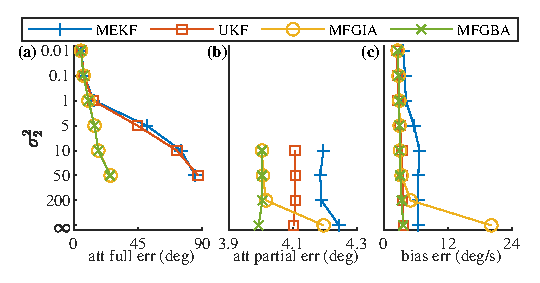
\includegraphics[scale=1.4]{figures/attEst-sim2-error}
	\caption{Estimation errors for varying accuracies of the second vector measurement: (a) full attitude error; (b) partial attitude error; (c) bias error for MEKF, UKF, MFGIA and MFGBA with varying $\sigma_2^2$.
		The errors of the unscented MFG filters are similar with the analytical MFG filters, and they are omitted for readability. \label{fig:attEst-sim2-error}}
\end{figure}

Six estimation schemes are compared, namely MEKF, UKF, two estimators with MFGB (one with the analytical propagation and the other with the unscented propagation, denoted respectively by MFGBA and MFGBU), and their counterparts with MFGI (denoted by MFGIA and MFGIU respectively).
For each case, one hundred Monte Carlo simulations (with respect to the random noise) are carried out.
Then, the attitude and bias errors are averaged across all time steps in one simulation, and further averaged across all simulations.
Paired $t$-tests ($N=100$, $\alpha=0.001$) are performed between MEKF, UKF and MFG filters, and between MFGB and MFGI to indicate any statistically significant difference.

The \textit{full} attitude error is defined as the angle between the true attitude and the estimated attitude.
As the second measurement becomes more inaccurate, the full attitude cannot be completely estimated because the rotation around the first reference vector becomes unobservable.
Thus, the \textit{partial} attitude error is defined as the angle between $R^T_t a_1$ and $R^Ta_1$, where $R_t$ and $R$ are the true attitude and the estimated attitude, respectively.
The partial attitude error only captures the accuracy along the first reference vector.
The simulation results are summarized in Table \ref{tab:attEst-sim2-error} and Fig. \ref{fig:attEst-sim2-error}.

When $\sigma_2^2 \in \{0.01,\ 0.1,\ 1\}$, the attitude error of the MFG filters is slightly lower than MEKF and UKF, and this advantage is mainly contributed by the faster initial convergence of MFG filters as illustrated in Fig. \ref{fig:attEst-sim2-trajectory-att}(a).
This is because for MEKF, the linearization of the measurement function is accurate only if the attitude error is small; and for UKF, the sigma points from a very large variance ($10^{10}$ in the initial step) suffer from the wrapping error, so they are unable to capture the large initial uncertainty.
The bias error of the MFG filters is also lower then MEKF, and is comparable to UKF (except when $\sigma_2^2=1$, UKF is statistically lower).

\begin{figure}
	\centering
	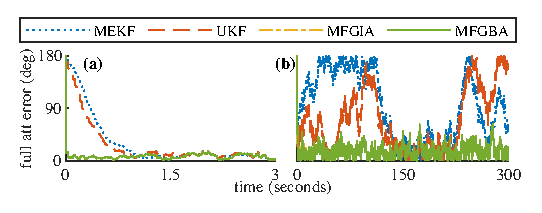
\includegraphics[scale=1.4]{figures/attEst-sim2-trajectory-att}
	\caption{(a) Full attitude error of MEKF, UKF, MFGIA and MFGBA for a sample simulation ($\sigma_2^2 = 0.1$) during the first three seconds.
		(b) Full attitude error (\SI{0}{\second} to \SI{300}{\second}) for a sample simulation ($\sigma_2^2 = 10$).
		The error of the unscented MFG filters is similar to the analytical MFG filters. \label{fig:attEst-sim2-trajectory-att}}.
\end{figure}

When $\sigma_2^2 \in \{5,\ 10,\ 50\}$, the full attitude error of the MFG filters is much lower than MEKF and UKF (Fig \ref{fig:attEst-sim2-trajectory-att}(b)).
This is because when the second vector measurement is inaccurate, the attitude uncertainty becomes highly dispersed along the rotation about the first reference vector, and the Gaussian distribution used by MEKF and UKF is incapable of modeling such large dispersion due to the wrapping error.
Also, the partial attitude error and bias error of the MFG filters are slightly lower than MEKF and UKF.
Next, comparing MFGB with MFGI, MFGB begins to exhibit some statistical advantages in partial attitude and bias errors, although their relative difference is still very small.
This difference can be attributed to that the attitude uncertainty becomes more non-isotropic as the second vector measurement becomes less accurate, so the distinction between the two definitions discussed in Chapter \ref{section:MFG-MFGI-MFGB} begins to emerge.
Because the gyroscope bias is resolved in the body-fixed frame, MFGB is more appropriate to model the correlation between attitude and bias than MFGI, this explains why the MFGB filter is more accurate.

When $\sigma_2^2 \in \{200,\ \infty\}$, MFGBA and MFGBU are still slightly more accurate than MEKF and UKF in partial attitude estimates, and more accurate than MEKF in bias estimation.
On the other hand, the performance of MFGIA and MFGIU in bias estimation degrades greatly, which affects the attitude error especially when $\sigma_2^2 = \infty$.
In Fig. \ref{fig:attEst-sim2-trajectory-bias}, the bias error of a sample simulation ($\sigma_2^2=\infty$) is shown, where MFGIA and MFGIU make little corrections to the bias.
It turns out that there is little correlation built between the bias and attitude for MFGI during the uncertainty propagation, indicating that the attitude-bias correlation with non-isotropic attitude measurements cannot be modeled properly with MFGI.

\begin{figure}
	\centering
	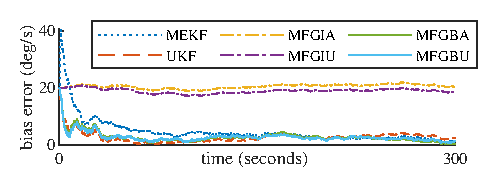
\includegraphics[scale=1.4]{figures/attEst-sim2-trajectory-bias}
	\caption{Bias error (\SI{0}{\second} to \SI{300}{\second}) in an example simulation ($\sigma_2^2=\infty$). \label{fig:attEst-sim2-trajectory-bias}}
\end{figure}

\paragraph{Magnetometer Measurement}

In this benchmark, a more realistic scenario is simulated where a satellite is orbiting around Earth with a single magnetometer and a gyroscope.
The orbital elements are given as follows, and three cases are considered for varying inclinations. 
\begin{equation*}
	a=6916\,\mathrm{km},\quad
	e=0.02,\quad
	\mathrm{\Omega} = 50^\circ,\quad
	\mathrm{\omega} = 0^\circ,\quad
	i = 0^\circ,\ 40^\circ \text{ or } 90^\circ.
\end{equation*}
According to the solution of the two-body problem, the orbital position with respect to the ECI frame, namely  $r_{ECI}\in\mathbb{R}^3$, is computed at each time step.

A 3U CubeSat with the mass of $m=\SI{3}{\kilogram}$ is considered. The inertia matrix is given by
\begin{equation*}
	J=\diag[0.0325,\; 0.0325,\; 0.005]\,\SI{}{\kilogram\meter^2}.
\end{equation*}
The true attitude and the true angular velocity, namely $(R_{ref},\Omega_{ref})$ are generated according to the Euler's equation of motion
\begin{gather*}
	J\dot\Omega_{ref} + \Omega_{ref}\times J\Omega_{ref} =0,\\
	\dot R_{ref} = R_{ref}\hat\Omega_{ref},
\end{gather*}
where the initial condition is chosen as
\begin{gather*}
	R_{ref}(0)=I_{3\times 3},\quad \Omega_{ref}(0)=[0.05,\; 0.05,\; 0.02]\,\SI{}{\radian\per\second}.
\end{gather*}
These are numerically integrated with the geometric numerical integrator preserving the structures of $\SO{3}$, referred to as the Lie group variational integrator~\cite{lee2007lie,lee2007lie-b}, using the time step of $\SI{0.05}{\second}$. 

It is assumed that the angular velocity measurement is measured by a gyroscope at $\SI{20}{\hertz}$, i.e., $h=\SI{0.05}{\second}$.
The noise parameters for the gyroscope are: (i) angle random walk: $H_u=0.1I_{3\times 3}$, and (ii) bias instability: $H_v=0.0005I_{3\times 3}$, as indicated in \eqref{eqn:attEst-kinematics-att} and \eqref{eqn:attEst-kinematics-bias}.
The initial bias of the gyroscope is set as $[0.01,\; 0.01,\; 0.01]\, \SI{}{\radian\per\second}$.

\begin{figure}
	\centering
	\begin{subfigure}[b]{0.28\textwidth}
		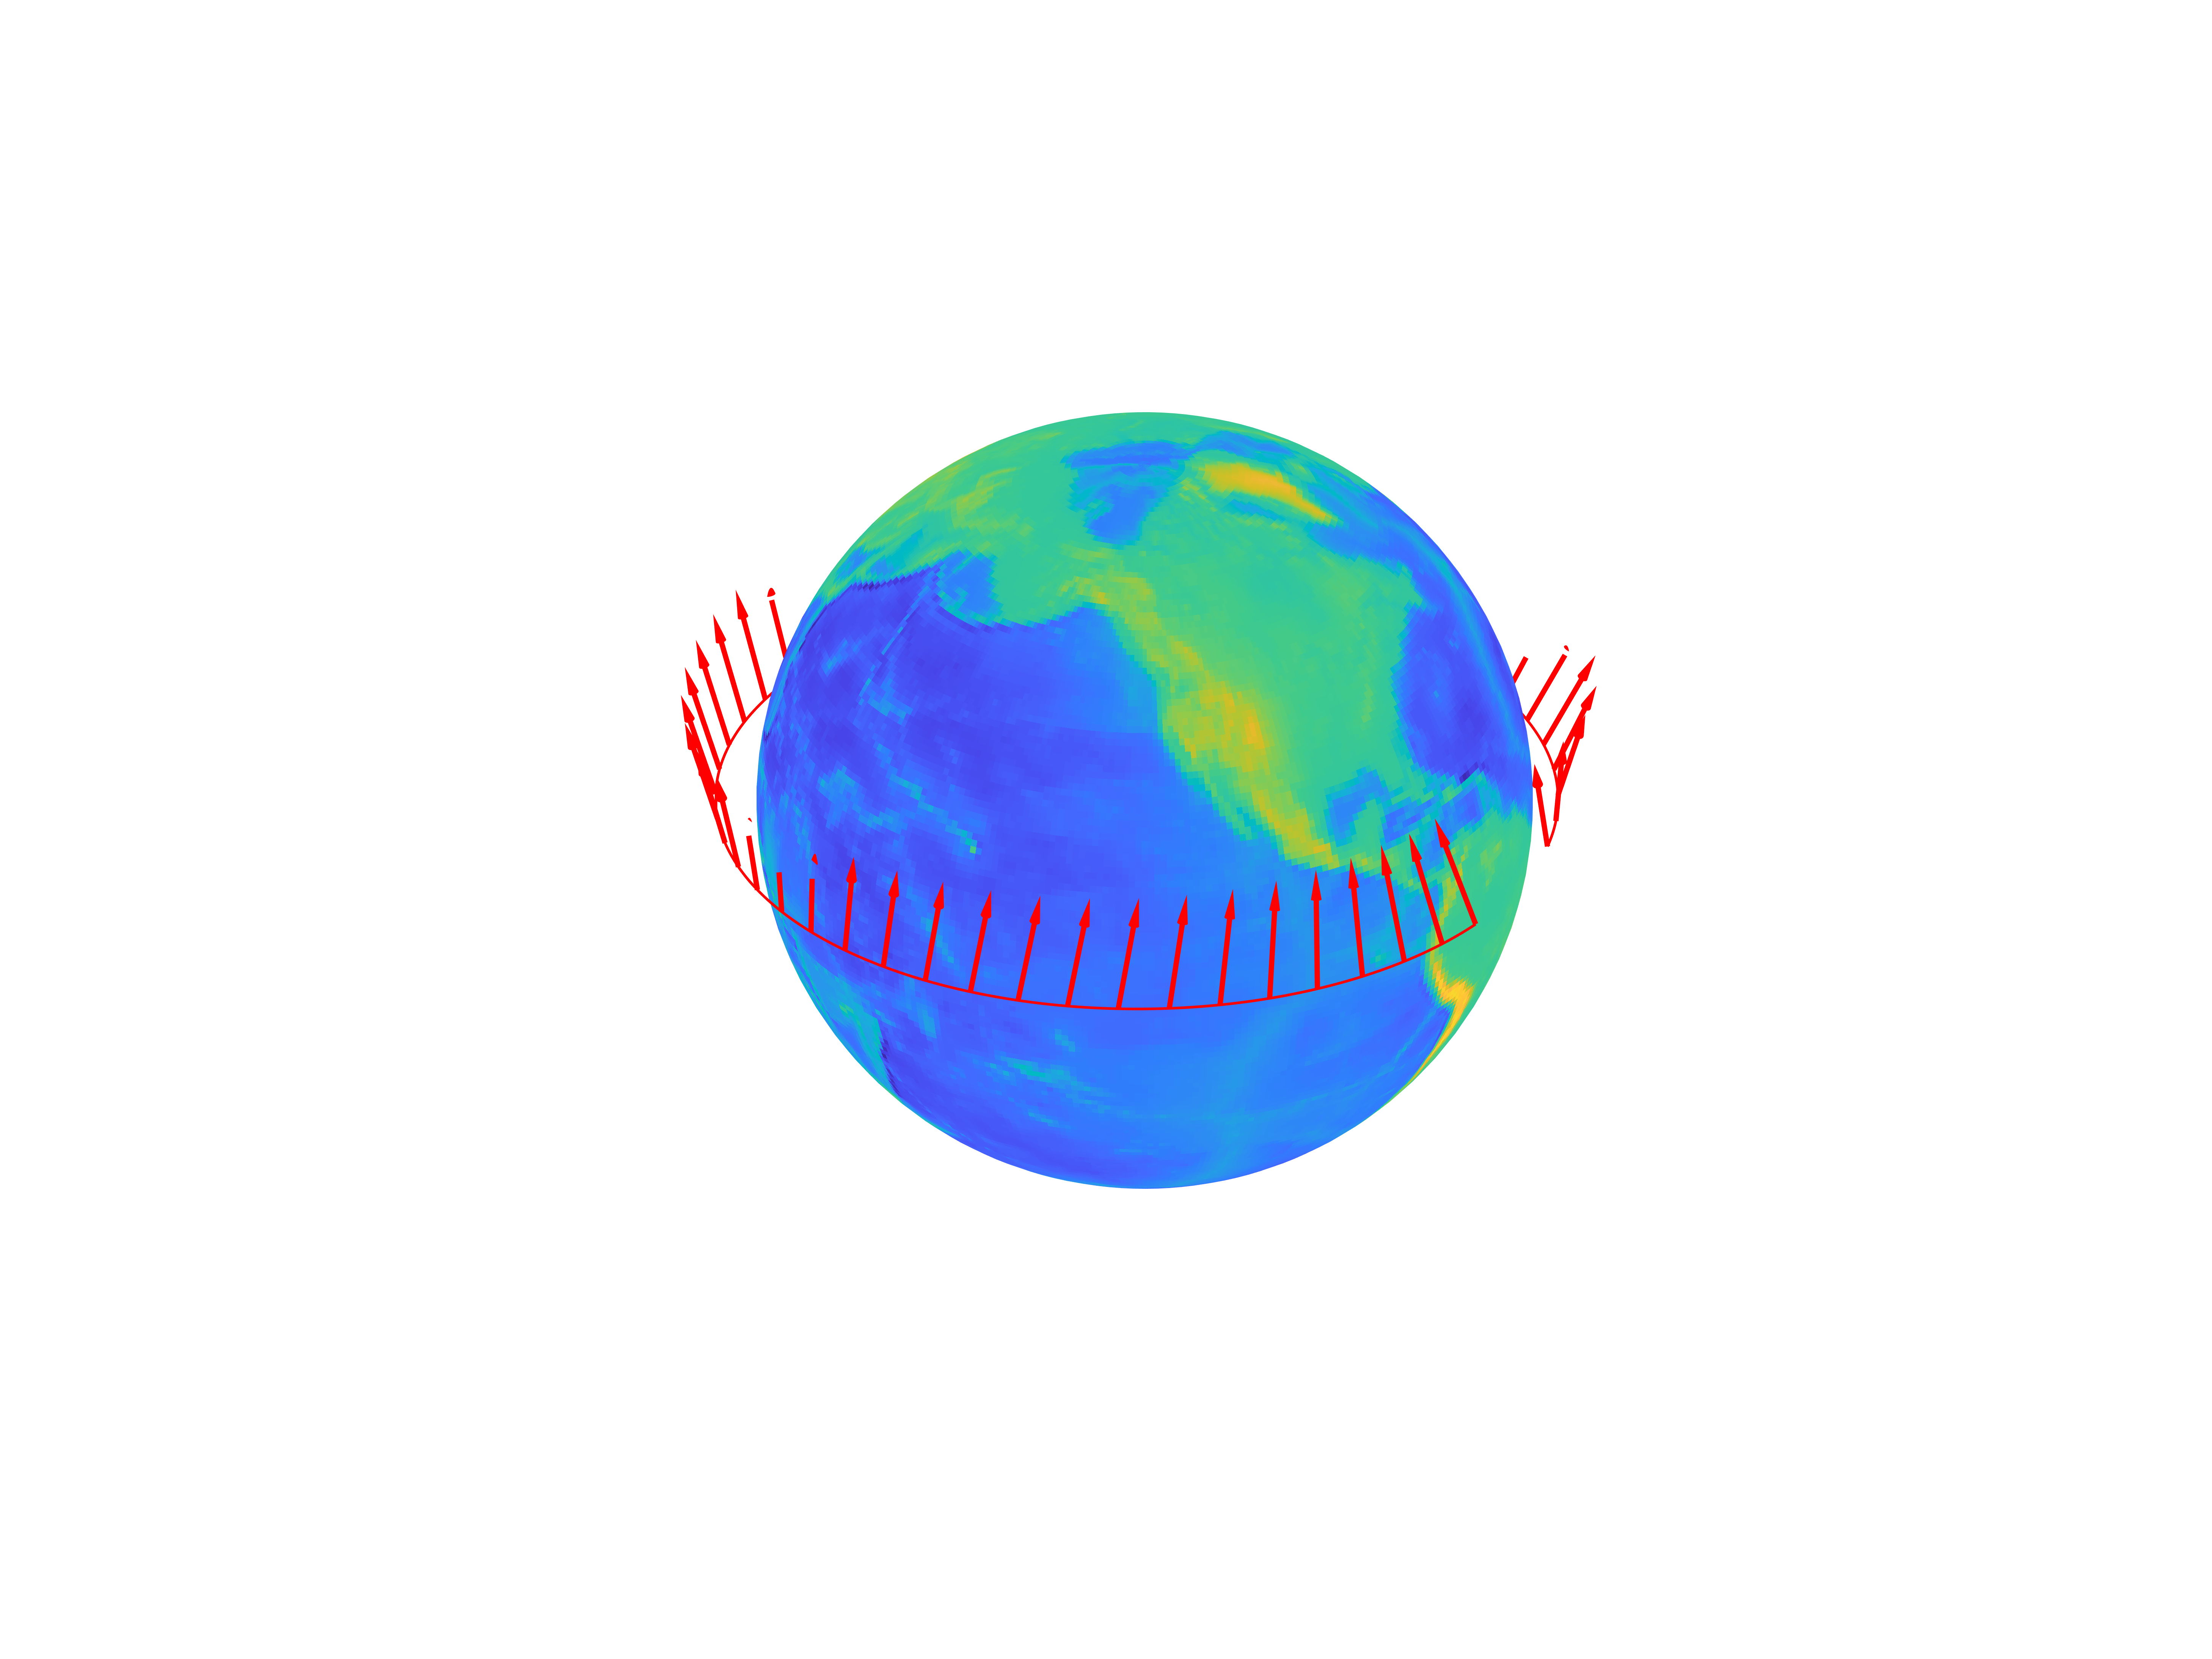
\includegraphics[trim={4.5cm 2.5cm 4cm 2.5cm},clip,width=1\textwidth]{figures/attEst-sim3-mag_0.png}
		\caption{$i=0^\circ$}
	\end{subfigure} \hspace{0.04\textwidth}
	\begin{subfigure}[b]{0.28\textwidth}
		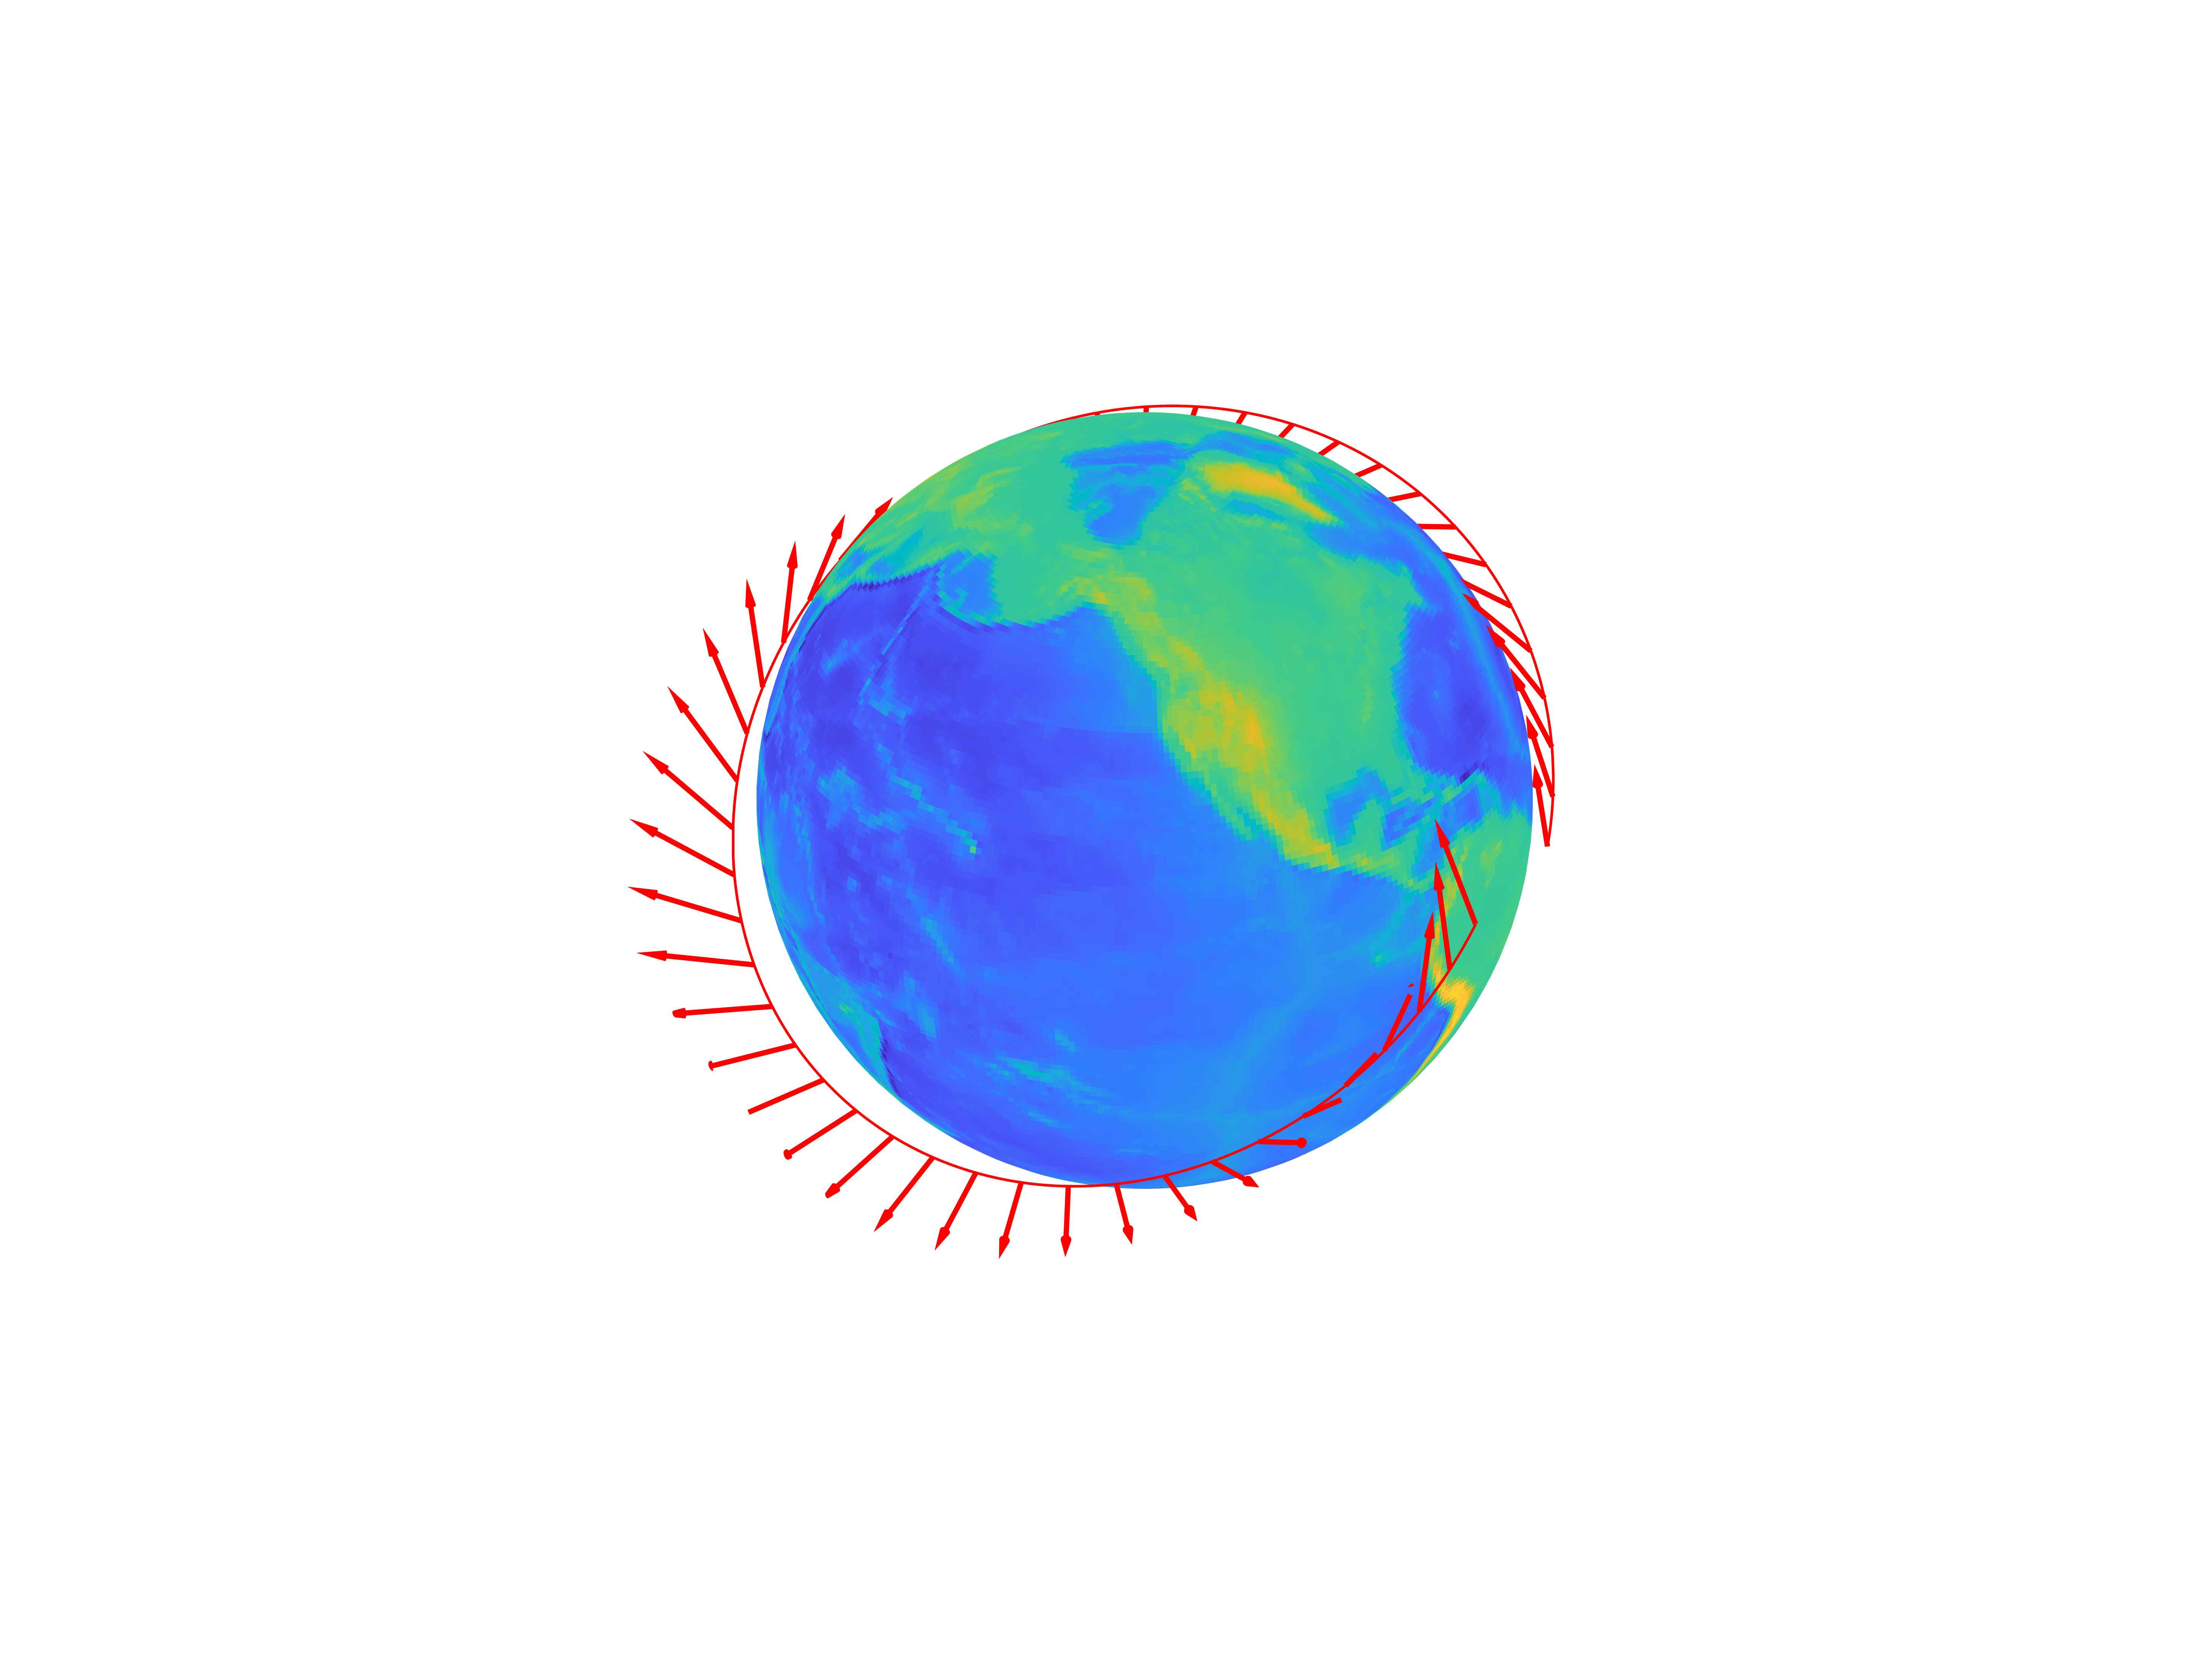
\includegraphics[trim={4.5cm 2.5cm 4cm 2.5cm},clip,width=1\textwidth]{figures/attEst-sim3-mag_40.png}
		\caption{$i=40^\circ$}
	\end{subfigure} \hspace{0.04\textwidth}
	\begin{subfigure}[b]{0.28\textwidth}
		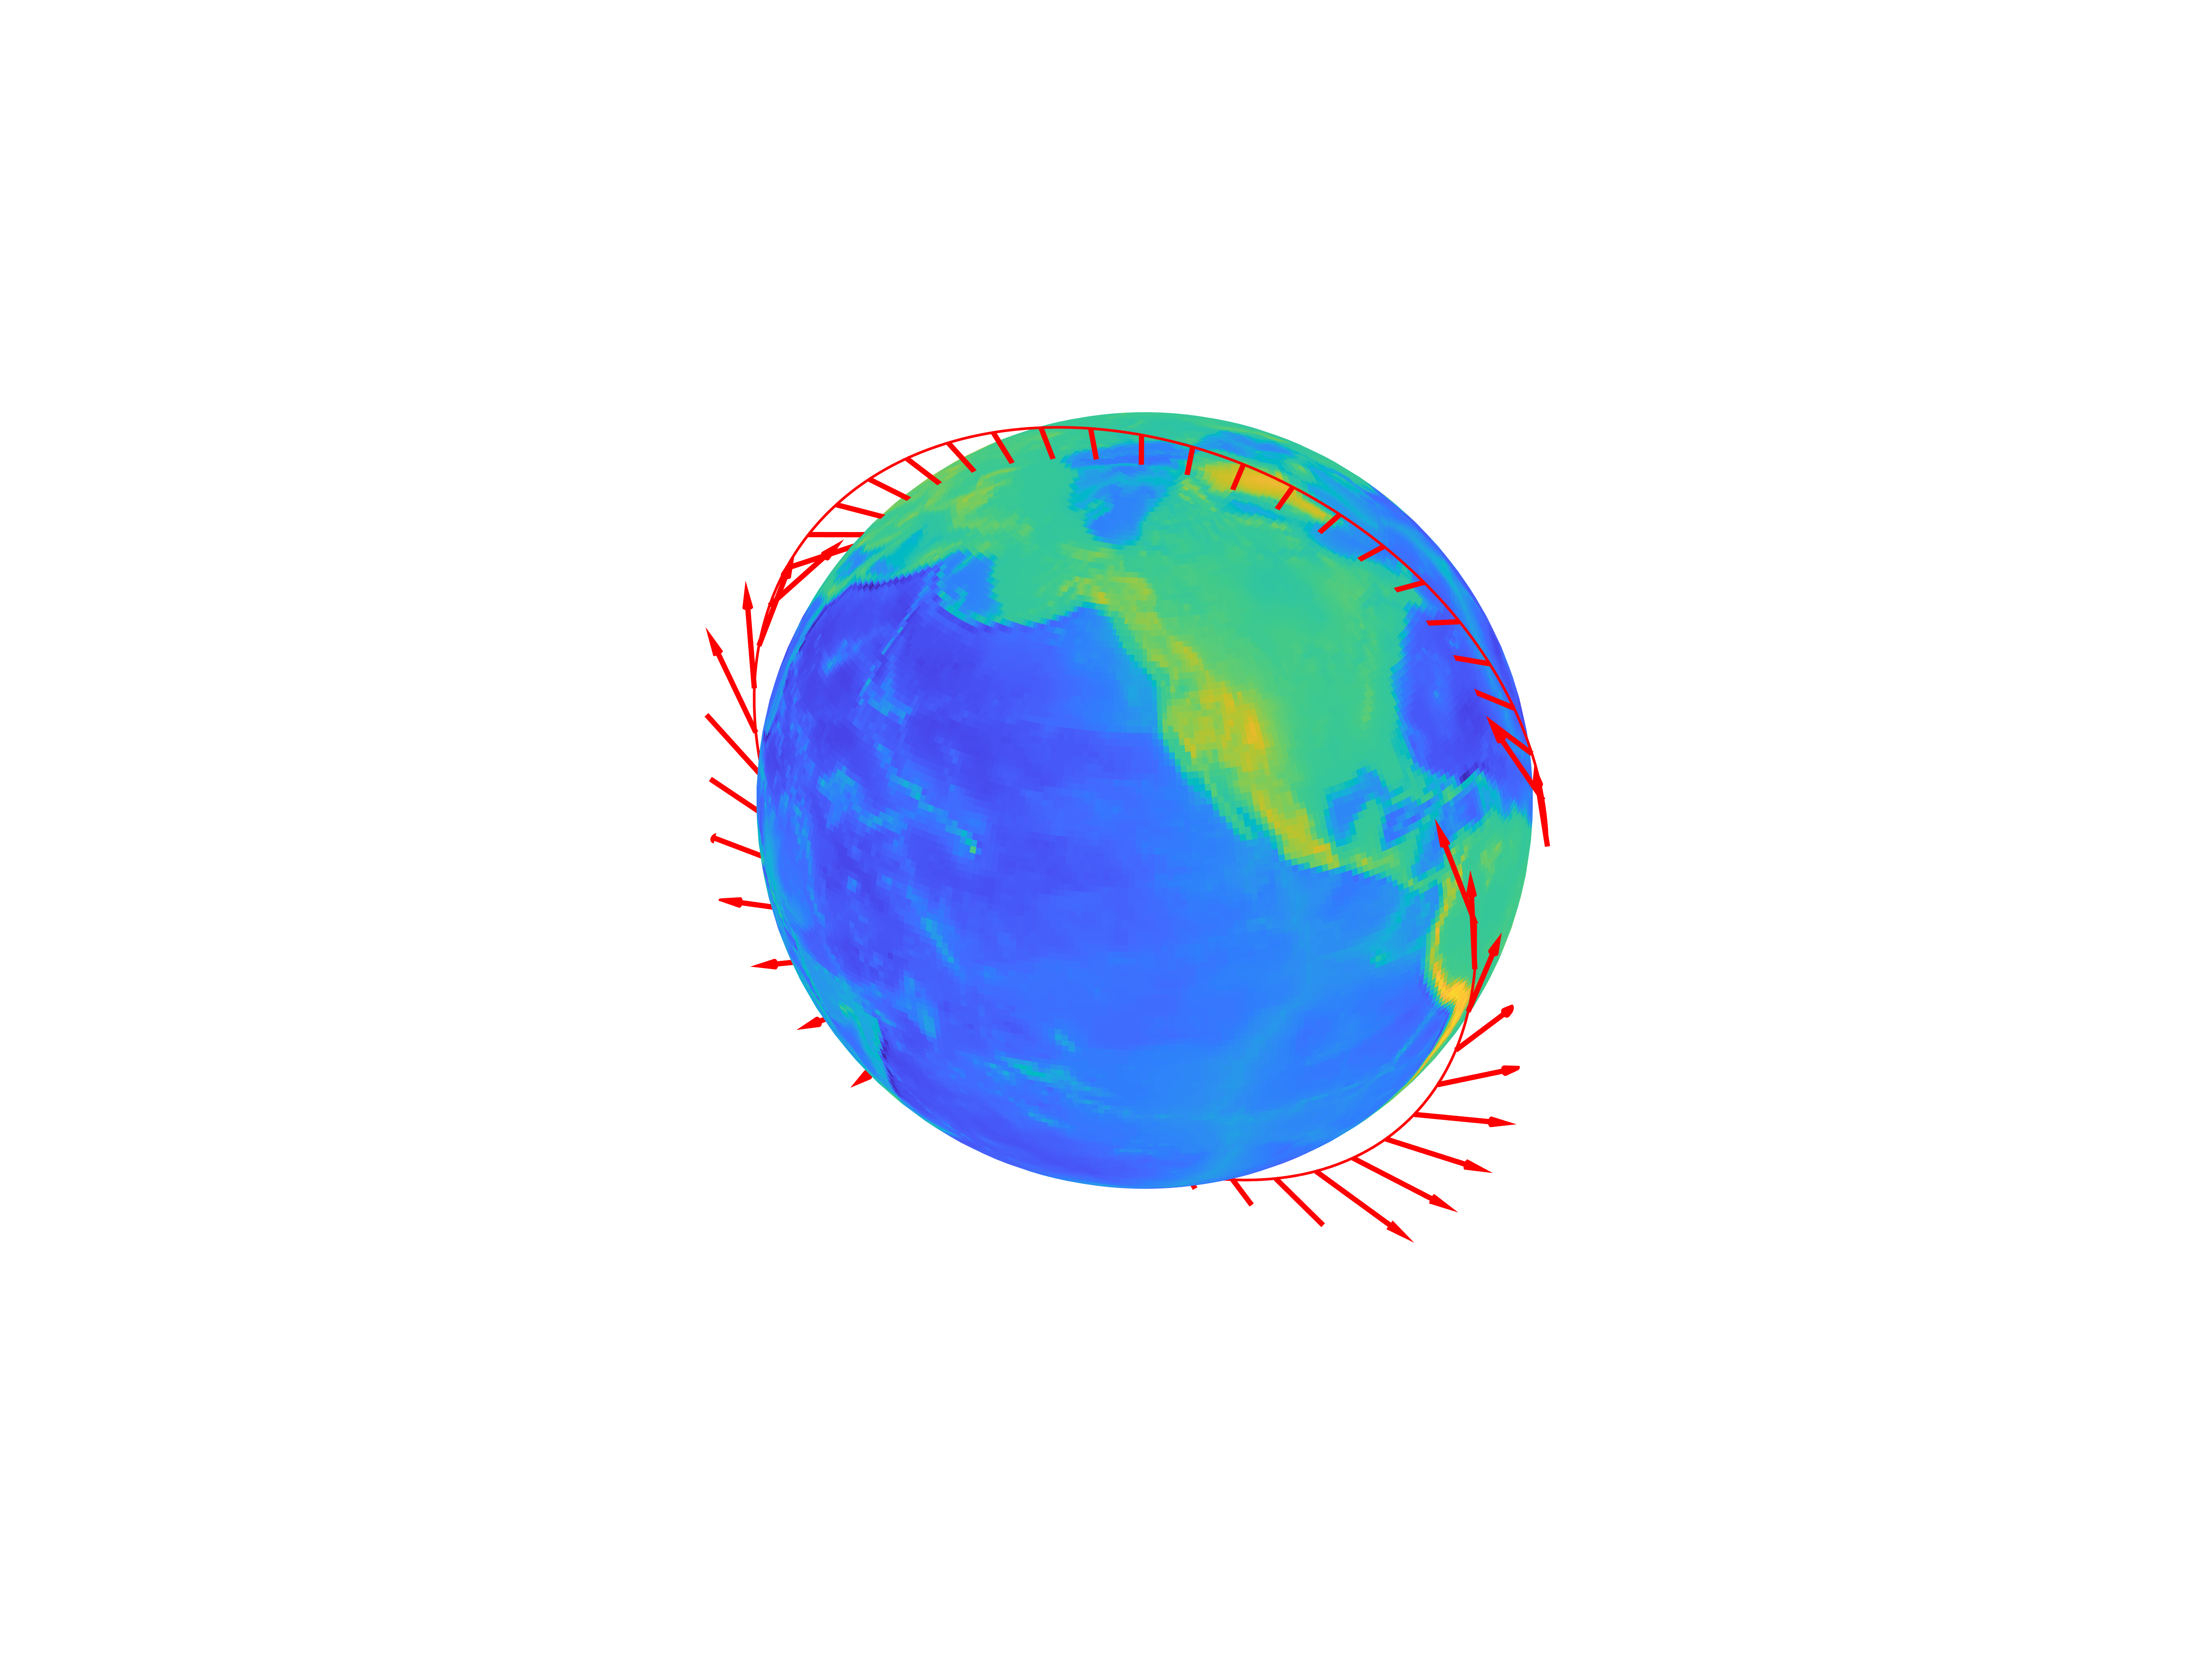
\includegraphics[trim={4.5cm 2.5cm 4cm 2.5cm},clip,width=1\textwidth]{figures/attEst-sim3-mag_90.png}
		\caption{$i=90^\circ$}
	\end{subfigure}
	\caption{Magnetic field on the orbit with different inclinations}
	\label{fig:attEst-sim3-magnetic}
\end{figure}

Next, the magnetometer measurements are generated as follows. 
Assuming that the simulation begins at the midnight of January 1, 2021, the orbital position in the ECI frame is transformed into the Earth-centered, Earth-fixed (ECEF) frame. 
This is because the Earth magnetic field is fixed to the ECEF frame. 
For the given location with respect to the ECEF frame, the Matlab function \texttt{wrldmagm} is called to compute the magnetic field.  
The Matlab function implements the NOAA World Magnetic Model presented in~\cite{chulliat2020us}. 
Then, the magnetic field is normalized to a unit-vector, which is transformed back to the ECI frame to obtain the true direction of the magnetic field at $t=t_k$, namely $a$ in \eqref{eqn:attEst-update-F}.
Figure \ref{fig:attEst-sim3-magnetic} illustrates the NOAA magnetic field model, where the magnetic field along the selected orbits with respect to the ECEF frame is shown.

The measurement from the magnetometer is assumed to be distributed according to the von Mises--Fisher distribution centered at the true magnetic field resolved in the body-fixed frame, namely $R^Tb\in\Sph^2$.
The concentration parameter $\kappa$ is chosen as $\kappa=200$. 
The average attitude error of the noisy magnetometer measurement is $5.08^\circ$, and it is assumed to be available also at \SI{20}{\hertz}.

Five filters are simulated to estimate the attitude and gyroscope bias of the spacecraft from gyroscope and magnetometer measurements, namely MEKF, two MFGB filters (MFGBA and MFGBU), and two MFGI filters (MFGIA and MFGIU).
The filters are initialized by
\begin{gather*}
	U_0 = \diag{[1,-1,-1]} \quad S_0 = 10I_{3\times 3} \quad V_0 = I_{3\times 3} \\
	\mu_0 = 0_{3\times 1} \quad \Sigma_0 = 0.01^2I_{3\times 3} \quad P_0 = 0_{3\times 3}.
\end{gather*}
The initial attitude estimation is the true attitude rotated by $180^\circ$ about its first body-fixed axis, and the initial bias estimation is off by $\SI{0.01}{\radian\per\second}$ in each axis.

Since there is only one direction measurement available from the magnetometer, the rotation of spacecraft about this reference vector is unobservable if the magnetic field is fixed.
Fortunately, as the spacecraft circles around Earth, the direction of the magnetic field changes at different locations (see Figure \ref{fig:attEst-sim3-magnetic}), and this allows the full attitude to be estimated \cite{grip2011attitude}.
However, since the magnetic field changes very slowly, estimating full attitude still remains very challenging.
Therefore, similar to the previous test, two attitude errors are defined: the full attitude error (FAE) at time $t_k$ is the angle that rotates $(R_{\mathrm{ref}})_k$ to $(R_{\mathrm{est}})_k$, and the partial attitude error (PAE) is the angle between $(R_{\mathrm{ref}})_k^Tb_k$ and $(R_{\mathrm{est}})_k^Tb_k$.
Note that the partial attitude error does not take into account the rotation about the reference vector $b_k$.

\begin{table*}
	\centering
	\caption{Estimation errors with magnetometer measurements \label{tab:attEst-sim3-estError}}
	\small
	\begin{tabular}{c|c|ccccc}
		\multicolumn{2}{c}{} & MEKF & MFGBA & MFGBU & MFGIA & MFGIU \\ \hline
		\multirow{3}{1.2cm}{$i=0^\circ$} & Attitude full error (deg) & 82.0 & 29.4 & 63.4 & 90.1 & 87.0 \\
		& Attitude partial error (deg) & 2.019 & 2.017 & 2.018 & 2.015 & 2.020 \\
		& Bias error (deg/s) & 0.313 & 0.044 & 0.045 & 0.119 & 1.366 \\ \hline
		\multirow{3}{1.2cm}{$i=40^\circ$} & Attitude full error (deg) & 85.0 & 8.7 & 25.7 & 22.0 & 82.9 \\
		& Attitude partial error (deg) & 2.018 & 2.016 & 2.019 & 2.015 & 2.020 \\
		& Bias error (deg/s) & 0.321 & 0.048 & 0.051 & 0.176 & 1.324 \\ \hline
		\multirow{3}{1.2cm}{$i=90^\circ$} & Attitude full error (deg) & 82.8 & 7.2 & 20.5 & 22.8 & 76.8 \\
		& Attitude partial error (deg) & 2.018 & 2.016 & 2.019 & 2.014 & 2.020 \\
		& Bias error (deg/s) & 0.298 & 0.053 & 0.060 & 0.252 & 1.178 \\ \hline
	\end{tabular}
\end{table*}

The estimation errors for the five filters are presented in Table \ref{tab:attEst-sim3-estError} and Figure \ref{fig:attEst-sim3-error-i0} to Figure \ref{fig:attEst-sim3-error-i90}.
In addition, the estimated uncertainties in attitude and bias are presented in Figure \ref{fig:attEst-sim3-error-i0} to Figure \ref{fig:attEst-sim3-error-i90}.
Looking at the bias estimation, the two MFGB based filters are much more accurate than MEKF, though their estimated uncertainties are similar.
Because the bias is represented in the body-fixed frame, MFGB is more appropriate then MFGI to model the attitude-bias correlation.
Therefore, MFGB based filters behave better than MFGI based filters, and this can also be seen from that the MFGB filters have lower bias uncertainty.
In particular, the MFGIU filter has the worst performance in bias estimation.

The partial attitude error is directly related to the magnetometer measurement, and is corrected in every time step.
Hence, it is relatively easy to estimate the partial attitude which is not involved with the rotation about the reference vector.
And as a result, all filters tested are able to estimate partial attitude with equally low estimation error.
Furthermore, the attitude uncertainties in the two axes perpendicular to the reference magnetic field are consistently low for all filters, though there appears to be more fluctuations for MEKF.
Also, the partial attitude error does not depend on the inclination angle $i$ of the orbit.

\begin{figure}
	\centering
	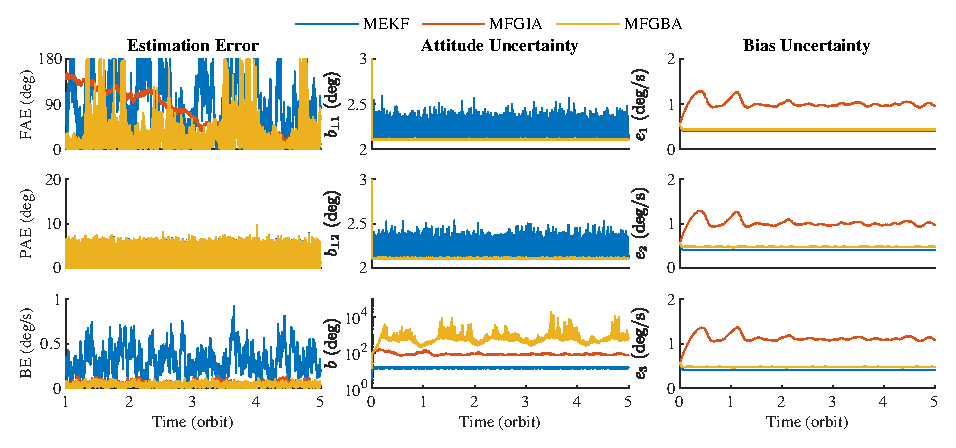
\includegraphics[scale=0.97]{figures/attEst-sim3-error-i0}
	\caption{Estimation error, attitude uncertainty, and bias uncertainty for various attitude filters when $i=0^\circ$.
		The attitude uncertainty is expressed in the coordinate frame specified by the direction of magnetic field ($b$), and its two perpendicular vectors ($b_{\perp 1}$ and $b_{\perp 2}$).
		The attitude uncertainty for MEKF is given by the square root of the diagonals of its covariance; and that for MFG filters is given by the square root of the diagonals of $(\tr{S}I_{3\times 3}-S)^{-1}$, after transformed into the correct frame.
		The bias uncertainty is expressed in the body-fixed frame, and is given by the square root of the diagonals of the covariance.
		The results for MFG unscented filters are omitted for better readability.}
	\label{fig:attEst-sim3-error-i0}
\end{figure}

\begin{figure}
	\centering
	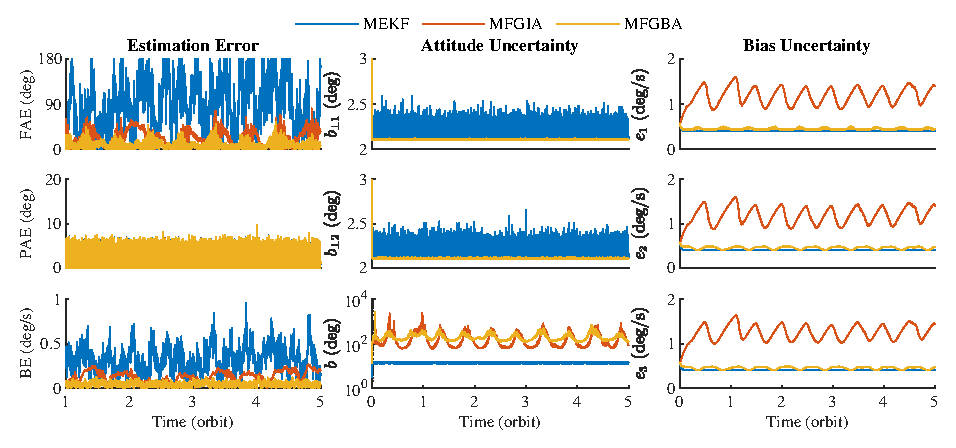
\includegraphics[scale=0.97]{figures/attEst-sim3-error-i40}
	\caption{Estimation error, attitude uncertainty, and bias uncertainty for various attitude filters when $i=40^\circ$.}
	\label{fig:attEst-sim3-error-i40}
\end{figure}

\begin{figure}
	\centering
	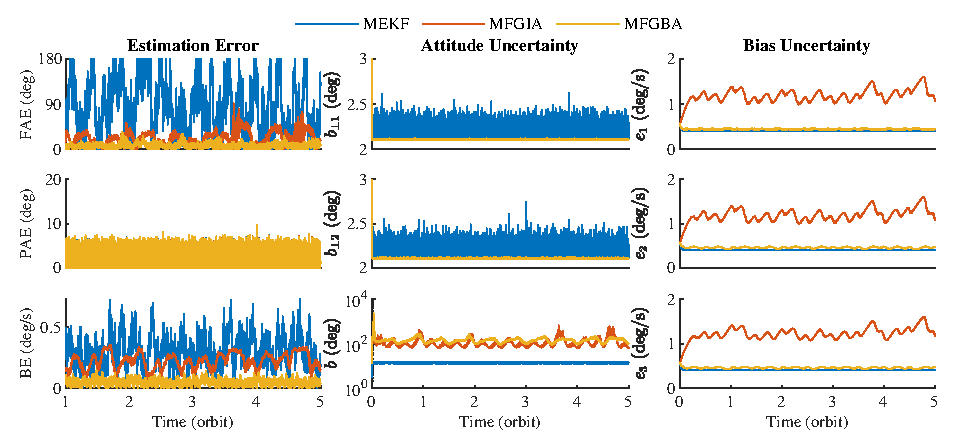
\includegraphics[scale=0.97]{figures/attEst-sim3-error-i90}
	\caption{Estimation error, attitude uncertainty, and bias uncertainty for various attitude filters when $i=90^\circ$.}
	\label{fig:attEst-sim3-error-i90}
\end{figure}

The full attitude is extremely challenging to estimate due to that the direction of magnetic field $b$ changes very slowly.
Among all tested filters, only the MFGB based filters (and in particular MFGBA) are able to give relatively low full attitude error.
Compared with the results in \cite{lee2019spacecraft} where the full attitude can be accurately estimated with a gyroscope and a single magnetometer, the difference here is the inclusion of a non-zero time varying gyroscope bias.
Because there is only one slow-varying reference vector, the integration accuracy of angular velocity from gyroscope is of crucial importance for full attitude estimation.
However, the inclusion of a time varying gyroscope bias deteriorates the integration accuracy very badly.
And therefore, the estimation accuracy of bias has a strong impact on the estimation of full attitude, and this explains why the MFGB based filters have lower full attitude error compared with other filters.
It is surprising that MEKF has the lowest attitude uncertainty in the reference magnetic field direction, nonetheless it is the least accurate in full attitude estimation.
This may reflect that the Gaussian distribution assumed by MEKF cannot properly model the large attitude dispersion due to the wrapping problem.
In addition, the analytical propagation for MFG filters behave consistently better than unscented propagation in full attitude estimation.
Also, because the direction of $b$ changes more quickly as the inclination angle $i$ is increased, the full attitude error also becomes lower.

\subsection{Summary}

In this section, the MFG defined in Chapter \ref{chap:MFG} is used to design an attitude estimator that is able to concurrently estimate the attitude and gyroscope bias.
Because MFG is defined intrinsically on $\SO{3}\times \mathbb{R}^n$, it is able to handle large attitude uncertainty.
Compared with the Gaussian based MEKF, the MFG filter does not show any advantage when the attitude uncertainty is small.
However, for challenging cases with large attitude uncertainty, for example, when the initial attitude is completely wrong, the MFG filters exhibit much faster convergence rate than MEKF.
Also, if there is a degree of freedom that is not properly observed, for example, when a direction measurement is very inaccurate, or when a single reference direction is slowly varying in the inertial frame, the MFG filters have better accuracy than MEKF.
Due to that the gyroscope bias is resolved in the body-fixed frame, the MFGB definition more accurately models the attitude-bias correlation than the MFGI definition.
The advantage of MFGB becomes particularly significant when the attitude uncertainty is highly non-isotropic, which is consistent with the discussion in Chapter \ref{section:MFG-MFGI-MFGB}.

\section{Loosely Coupled IMU-GNSS Integration}

In this section, the attitude estimation problem considered in the previous section is extended into a full inertial navigation problem.
More specifically, it is assumed that an inertial measurement unit (IMU) is attached to a rigid body, which has a gyroscope measuring the angular velocity, and an accelerometer measuring the linear acceleration, both in the body fixed frame.
The linear acceleration can be transformed into the inertial frame using the integrated attitude, and then it can be integrated twice into position after subtracting the gravity component.
It is also assumed that a global navigation satellite system (GNSS) receiver provides position measurements of the rigid body, which are used to correct the attitude and position integrated using the IMU.
Since the pseudorange from GNSS is first converted into position measurements, and then used to correct the inertial navigation estimation, this is usually referred to as loosely coupled IMU-GNSS integration.

The MEKF for attitude estimation can be generalized to deal with this inertial navigation setting \cite{sola2017quaternion}.
However, as discussed in previous sections, it cannot handle large attitude uncertainty due to its inherent Gaussian assumption.
Similar as in attitude estimation, the MFG is used to design a new estimator, which is suitable for large attitude uncertainty.
This is particularly advantageous in some practical problems, for example, when the IMU starts in a building, where the heading direction is usually completely unknown; or when the GNSS receiver cannot receive signal for a long period time, and the uncertainty for inertial navigation accumulates.

The definition of MFG is flexible enough to handle this inertial navigation setting, as its linear part can be arbitrary in $\mathbb{R}^n$.
This makes MFG distinguished from the distribution defined for dual quaternions \cite{li2019geometry,li2020unscented}, where the linear part must be position only.
In this section, the MFG is used to design a Bayesian filter that estimates attitude, gyroscope bias, position, linear velocity, and accelerometer bias concurrently.

\subsection{Problem Formulation}

The IMU kinematic model is formulated in discrete time as follows
\begin{align}
	R_{k+1} &= R_k \expb{ h(\hat{\Omega}_k + \hat{b}_{g,k}) + H_{gu}\Delta W_{gu} }, \label{eqn:posEst-kinematics-attitude} \\
	b_{g,k+1} &= b_{g,k} + H_{gv}\Delta W_{gv}, \label{eqn:posEst-kinematics-gyrobias} \\
	p_{k+1} &= p_k + hv_k, \label{eqn:posEst-kinematics-pos} \\
	v_{k+1} &= v_k - gh + R_k\left( h(a_k+b_{a,k}) + H_{au}\Delta W_{au} \right), \label{eqn:posEst-kinematics-velocity} \\
	b_{a,k+1} &= b_{a,k} + H_{av}\Delta W_{av}, \label{eqn:posEst-kinematics-accebias}
\end{align}
where $R\in\SO{3}$ is the attitude, $x = \big[b_g^T, p^T, v^T, b_a^T\big]^T \in \mathbb{R}^{12}$ are gyroscope bias, position, linear velocity in inertial frame, and accelerometer bias, respectively.
The gravity vector is denoted by $g\in\mathbb{R}^3$.
Next, $\Omega\in\mathbb{R}^3$ is the angular velocity measured by the gyroscope, and $a\in\mathbb{R}^3$ is the linear acceleration measured by the accelerometer, and they are resolved in the body-fixed frame.
The angular velocity measurement is affected by two noises: $H_{gu}\Delta W_{gu}$ is a white noise, and $b_g$ is a random walk bias driven by $H_{gv}\Delta W_{gv}$.
The noises for accelerometer are similar, given by the white noise $H_{au}\Delta W_{au}$, and the bias driven by $H_{av}\Delta W_{av}$.
These noise terms are Gaussian with
\begin{align}
	&H_{gu}\Delta W_{gu} \sim \mathcal{N}(0,hG_{gu}), \quad H_{gv}\Delta W_{gv} \sim \mathcal{N}(0,hG_{gv}), \label{eqn:posEst-gyroNoise} \\
	&H_{au}\Delta W_{au} \sim \mathcal{N}(0,hG_{au}), \quad H_{av}\Delta W_{av} \sim \mathcal{N}(0,hG_{av}),
\end{align}
where $G_{gu} = H_{gu}H_{gu}^T$, $G_{gv} = H_{gv}H_{gv}^T$, $G_{au} = H_{au}H_{au}^T$, $G_{av} = H_{av}H_{av}^T$, and they are independent.
Finally, the subscript $k$ denote the time step, and $h = t_{k+1}-t_k$ is constant sampling period for any $k$.

It is assumed that the position $p_k$ is measured by a GNSS receiver at time $t_k$, denote by $y_k\in\mathbb{R}^3$.
The measurement noise is Gaussian, i.e.,
\begin{align}
	y_k|p_k = p_k + \mathcal{N}(0,\Sigma_y).
\end{align}
Optionally, the attitude and some reference directions can also be measured as formulated in Chapter \ref{section:attEst-problem}.
Namely, the attitude can be directly measured by $N_a$ sensors as $Z_i$, and the measurement noises follow matrix Fisher distributions with parameters $F_{Z_i}$, for $i=1,\ldots,N_a$.
Also, $N_v$ fixed reference directions $a_j\in\Sph^2$ in inertial frame are measured as $z_j\in\Sph^2$ in the body-fixed frame, and the measurement noises follow von Mises-Fisher distribution with the mean direction $R_t^TB_ja_j$, and concentration parameter $\kappa$, where $R_t\in\SO{3}$ is the true attitude, for $j = 1,\ldots,N_v$.
All measurements at time $t_k$ are denoted by $\mathcal{Z}_k$.

Suppose $(R_0,x_0) = (R_0,b_{g,0},p_0,v_0,b_{a,0})$ at the initial time $t_0$ follow an MFG with $n=12$ and parameters $(\mu_0,\Sigma_0,P_0,U_0,S_0,V_0)$.
Given the IMU measurements $\{\Omega_k,a_k\}_{k=1}^\infty$, and all position, attitude, and direction measurements $\mathcal{Z}_{k=1}^\infty$, the problem is to find the posterior distribution of $(R_k,x_k) | \{\mathcal{Z}_m\}_{m=1}^k$, and approximate it to an MFG with parameters $(\mu_k, \Sigma_k, P_k, U_k, S_k, V_k)$.
Similar to the attitude estimator, two steps are needed.
In the uncertainty propagation step, the posterior distribution $(R_k,x_k) | \{\mathcal{Z}_m\}_{m=1}^k$ is propagated using the IMU kinematic equations \eqref{eqn:posEst-kinematics-attitude}-\eqref{eqn:posEst-kinematics-accebias} to the next time step as $(R_{k+1},x_{k+1}) | \{\mathcal{Z}_m\}_{m=1}^k$.
Next, the propagated distribution is updated by the measurements $\mathcal{Z}_{k+1}$ using Bayes' formula into $(R_{k+1},x_{k+1}) | \{\mathcal{Z}_m\}_{m=1}^{k+1}$.
In the next two subsections, algorithms for these two steps are developed.

\subsection{Uncertainty Propagation} \label{section:posEst-propagation}

Suppose $(R_k,x_k) | \{\mathcal{Z}_m\}_{m=1}^k \sim \mathcal{MG}(\mu_k, \Sigma_k, P_k, U_k, S_k, V_k)$.
In this subsection, the moments of $(R_{k+1},x_{k+1})$ required for the MLE of MFG are calculated using the IMU kinematics equations \eqref{eqn:posEst-kinematics-attitude}-\eqref{eqn:posEst-kinematics-accebias}.
One way of calculating those moments is to propagated deterministically sampled sigma points through the kinematic equations using the unscented transform of MFG, as introduced in Chapter \ref{section:attEst-propagation}.
This approach can be easily generalized to the inertial navigation settings considered in this subsection, and will not be discussed here.
Instead, this subsection calculates approximate analytical expressions of the required moments.

First, because \eqref{eqn:posEst-kinematics-attitude} and \eqref{eqn:posEst-kinematics-gyrobias} are exactly the same as the attitude kinematics considered in \eqref{eqn:attEst-kinematics-att-dist} and \eqref{eqn:attEst-kinematics-bias-dist}, the moment $\expect{R_{k+1}}$ can be calculated using Theorem \ref{thm:attEst-prop-E(R_{k+1})}.
Then $\expect{R_{k+1}}$ is used in the marginal MLE of MFG to obtain the parameters $U_{k+1}$, $S_{k+1}$, and $V_{k+1}$.
Next, define $Q_{k+1} = U_{k+1}^TR_{k+1}V_{k+1}$, and $\nu_{R_{k+1}} = (Q_{k+1}S_{k+1}-S_{k+1}Q_{k+1}^T)^\vee$ for MFGI, or $\nu_{R_{k+1}} = (S_{k+1}Q_{k+1}-Q_{k+1}^TS_{k+1})^\vee$ for MFGB as the intermediate parameters for the MFG at time $t_{k+1}$.
According to Theorem \ref{thm:MFG-MLE-conditional}, $\expect{x_{k+1}}$, $\expect{x_{k+1}\nu_{R_{k+1}}^T}$, $\expect{x_{k+1}x_{k+1}^T}$, and $\expect{\nu_{R_{k+1}}\nu_{R_{k+1}}^T}$ need to be calculated.
Note that $\expect{\nu_{R_{k+1}}\nu_{R_{k+1}}^T}$ is only involved with the gyroscope kinematics \eqref{eqn:posEst-kinematics-attitude} and \eqref{eqn:posEst-kinematics-gyrobias}, so it can be calculated using \eqref{eqn:attEst-prop-EvRvR_{k+1}} in Theorem \ref{thm:attEst-prop-otherMoments}.
In the remainder of this subsection, the calculations for $\expect{x_{k+1}}$, $\expect{x_{k+1}\nu_{R_{k+1}}^T}$, and $\expect{x_{k+1}x_{k+1}^T}$ are developed.

In perpetration for these calculations, the parameters $\mu_k$, $P_k$ and $\Sigma_k$ are written for each component in block form as
\begin{gather} \label{eqn:posEst-prop-blocks}
	\allowdisplaybreaks
	\mu_k = \begin{bmatrix}
		\mu_{b_g,k} \\ \mu_{p,k} \\ \mu_{v,k} \\ \mu_{b_a,k}
	\end{bmatrix}, \qquad
	P_k = \begin{bmatrix}
		P_{b_g,k} \\ P_{p,k} \\ P_{v,k} \\ P_{b_a,k}
	\end{bmatrix}, \qquad
	\Sigma_k = \begin{bmatrix}
		\Sigma_{b_gb_g,k} & \Sigma_{b_gp,k} & \Sigma_{b_gv,k} & \Sigma_{b_gb_a,k} \\
		\Sigma_{pb_g,k} & \Sigma_{pp,k} & \Sigma_{pv,k} & \Sigma_{pb_a,k} \\
		\Sigma_{vb_g,k} & \Sigma_{vp,k} & \Sigma_{vv,k} & \Sigma_{vb_a,k} \\
		\Sigma_{b_ab_g,k} & \Sigma_{b_ap,k} & \Sigma_{b_av,k} & \Sigma_{b_ab_a,k}
	\end{bmatrix}.
\end{gather}
With these, the calculation for $\expect{x_{k+1}}$ is presented in the next theorem.

\begin{theorem} \label{thm:posEst-prop-Ex}
	The moment $\expect{x_{k+1}} = \expect{ b_{g,k+1}^T, p_{k+1}^T, v_{k+1}^T, b_{a,k+1}^T}^T$ are given by
	\begin{align}
		\expect{b_{g,k+1}} &= \expect{b_{g,k}} \\
		\expect{p_{k+1}} &= \expect{p_k} + h\expect{v_k} \\
		\expect{v_{k+1}} &= \expect{v_k} + h\expect{R_k}(a(0)+\mu_{b_a,k}) + h\expect{R_kP_{b_a,k}\nu_{R_k}} - gh, \\
		\expect{b_{a,k+1}} &= \expect{b_{a,k}}
	\end{align}
	where $\nu_{R_k} = (Q_kS_k-S_kQ_k^T)^\vee$ for MFGI, or $\nu_{R_k} = (S_kQ_k-Q_k^TS_k)^\vee$ for MFGB, with $Q_k = U_k^TR_kU_k$.
\end{theorem}
\begin{proof}
	The first, second, and fourth equations are immediate from \eqref{eqn:posEst-kinematics-gyrobias}, \eqref{eqn:posEst-kinematics-pos}, and \eqref{eqn:posEst-kinematics-accebias}, because $\Delta W_{gv}$ and $\Delta W_{av}$ have zeros means.
	For the third equation, a similar calculation as \eqref{eqn:MFG-Exx-proof} shows that
	\begin{align*}
		\expect{R_kb_{a,k}} = \expect{R_k}\mu_{b_a,k} + \expect{R_kP_{b_a,k}\nu_{R_k}},
	\end{align*}
	and the desired result is proved.
\end{proof}

The expressions for $\expect{x_{k+1}\nu_{R_{k+1}}^T}$ and $\expect{x_{k+1}x_{k+1}^T}$ are very tedious, and they are relegated to Appendix \ref{app:posEst-prop-moments}.
Note that these two moments, $\expect{\nu_{R_{k+1}}\nu_{R_{k+1}}^T}$, and $\expect{x_{k+1}}$ can be calculated using up to the third order moments of $Q_k\sim\mathcal{M}(S_k)$, with the accuracy of $O(h^2)$.
Then using Theorem \ref{thm:MFG-MLE-conditional}, the parameters $\mu_{k+1}$, $P_{k+1}$ and $\Sigma_{k+1}$ can be obtained.
In summary, the uncertainty $S(R_k,x_k) \sim \mathcal{MG}(\mu_k, \Sigma_k, P_k, U_k, S_k, V_k)$ at time $t_k$ is propagated into $(R_{k+1},x_{k+1}) \sim \mathcal{MG}(\mu_{k+1},\allowbreak \Sigma_{k+1},\allowbreak P_{k+1},\allowbreak U_{k+1},\allowbreak S_{k+1},\allowbreak V_{k+1})$, up to accuracy $O(h^2)$ in moments.
The pseudocode for this uncertainty propagation scheme is summarized in Table \ref{tab:posEst-prop}.

\begin{table}
	\caption{Uncertainty propagation for IMU kinematics}
	\label{tab:posEst-prop}
	\begin{algorithmic}[1]
		\algrule[0.8pt]
		\Procedure{$\mathcal{MG}(t_{k+1}) = $ Uncertainty Propagation}{$\mathcal{MG}(t_k),\Omega_k,a_k$}
		\algrule
		\State Calculate $\expect{R_{k+1}}$ using \eqref{eqn:attEst-prop-E(R_{k+1})} with $\mu_k$, $P_k$, $G_u$ replaced by $\mu_{b_g,k}$, $P_{b_g,k}$ in \eqref{eqn:posEst-prop-blocks}, and $G_{gu}$ in \eqref{eqn:posEst-gyroNoise}, respectively.
		\State Obtain $U_{k+1},S_{k+1},V_{k+1}$ according to Chapter \ref{section:MFG-property} using $\expect{R_{k+1}}$.
		\State Calculate $\expect{\nu_{R_{k+1}}\nu_{R_{k+1}}^T}$ using \eqref{eqn:attEst-prop-EvRvR_{k+1}}, calculate $\expect{x_{k+1}}$, $\expect{x_{k+1}\nu_{R_{k+1}}^T}$ and $\expect{x_{k+1}x_{k+1}^T}$ with Theorem \ref{thm:posEst-prop-Ex}, Theorem \ref{thm:posEst-prop-ExvR}, and Theorem \ref{thm:posEst-prop-Exx}, respectively.
		\State Obtain $\mu_{k+1},\Sigma_{k+1},P_{k+1}$ according to Theorem \ref{thm:MFG-MLE-conditional} using the moments calculated in Step 4.
		\State Set $\mathcal{MG}(t_{k+1}) = \mathcal{MG}(\mu_{k+1},\Sigma_{k+1},P_{k+1},U_{k+1},S_{k+1},V_{k+1})$.
		\EndProcedure
		\algrule[0.8pt]
	\end{algorithmic}
\end{table}

\subsection{Measurement Update}

The algorithm for propagating the posterior distribution $(R_k,x_k) | \{\mathcal{Z}_{m}\}_{m=1}^k$ at time $t_k$ into the prior distribution $(R_{k+1},x_{k+1}) | \{\mathcal{Z}_{m}\}_{m=1}^k$ at time $t_{k+1}$ has been introduced in the previous subsection.
In this subsection, the prior distribution $(R_{k+1},x_{k+1}) | \{\mathcal{Z}_{m}\}_{m=1}^k$ is updated into the posterior distribution $(R_{k+1},x_{k+1}) | \{\mathcal{Z}_{m}\}_{m=1}^{k+1}$ at time $t_{k+1}$, with the measurements $\mathcal{Z}_{k+1}$ using Bayes' formula.
Since the update is completed instantaneously at time $t_{k+1}$, the subscript $k+1$ is omitted in this subsection, and the variables relevant to the posterior distribution are denoted by the superscript $+$.

Suppose the prior distribution of $(R,x)$ before measurement update follows MFG with parameters $(\mu,\Sigma,P,U,S,V)$. 
By the Bayes' rule and Theorem 3.2 in \cite{lee2018bayesian}, the posterior density conditioned on all of the available measurements $\mathcal{Z}$ is 
\begin{align} \label{eqn:posEst-update-density}
	&p(R,x\lvert \mathcal{Z}) \propto \etr{ \bigg( F + \sum_{i=1}^{N_a}Z_iF_i^T + \sum_{j=1}^{N_v}\kappa_jB_ja_jz_j^T \bigg)R^T } \nonumber \\
	&\quad \cdot \expb{-\tfrac{1}{2}(x-\mu_c)^T\Sigma_c^{-1}(x-\mu_c)} \cdot \expb{-\tfrac{1}{2}(Hx-y)^T\Sigma_y^{-1}(Hx-y)},
\end{align}
where $H = [0_{3\times 3}, I_{3\times 3}, 0_{3\times 6}]$ selects the position component from $x$, and $F$, $\mu_c$ and $\Sigma_c$ are defined as in Definition \ref{def:MFG} with respect to $(\mu,\Sigma,P,U,S,V)$.
Compared with \eqref{eqn:attEst-update-density} in attitude estimation, \eqref{eqn:posEst-update-density} has an additional term contributed by the position measurement coming from the GNSS receiver.

To deal with this posterior density, it is first shown that \eqref{eqn:posEst-update-density} can be factorized into the marginal component for $R$, and the conditional component for $x|R$.
\begin{lemma}
	Let $\tilde{F}$ be defined as the $F^+$ in \eqref{eqn:attEst-update-F}, or $\tilde{F} = F$ if there is no attitude or direction measurements.
	Also, define the ``Kalman gain''
	\begin{align}
		K = \Sigma_cH^T(H\Sigma_cH^T + \Sigma_y)^{-1} \in \mathbb{R}^{12\times 3}.
	\end{align}
	Then the posterior density \eqref{eqn:posEst-update-density} can be factorized into two parts:
	\begin{align} \label{eqn:posEst-update-density-factor}
		p(R,x|\mathcal{Z}) = f_R(R) f_{x|R}(x|R),
	\end{align}
	where the marginal part $f_R(R)$ is given by
	\begin{align} \label{eqn:posEst-update-density-R}
		f_R(R) \propto \etr{\tilde{F}R^T} \expb{-\tfrac{1}{2}(H\mu_c-y)^T (\Sigma_y+H\Sigma_cH^T)^{-1} (H\mu_c-y)},
	\end{align}
	and the conditional part $f(x|R)$ is given by
	\begin{align} \label{eqn:posEst-update-density-x|R}
		f_{x|R}(x|R) \propto \expb{-\tfrac{1}{2} \big(x-(I-KH)\mu_c-Ky\big)^T \big((I-KH)\Sigma_c\big)^{-1} \big(x-(I-KH)\mu_c-Ky\big)},
	\end{align}
	where $I$ is abbreviated for $I_{12\times 12}$.
\end{lemma}
\begin{proof}
	Using a similar technique that is used to prove the linear Kalman filter, and the Woodbury matrix identity \cite{petersen2008matrix}, it can be proved that
	\begin{align*}
		&\expb{-\tfrac{1}{2}(x-\mu_c)^T\Sigma_c^{-1}(x-\mu_c)} \cdot \expb{-\tfrac{1}{2}(Hx-y)^T\Sigma_y^{-1}(Hx-y)} \\
		= &\expb{-\tfrac{1}{2} \big(x-(I-KH)\mu_c-Ky\big)^T \big((I-KH)\Sigma_c\big)^{-1} \big(x-(I-KH)\mu_c-Ky\big)} \\
		&\qquad \cdot \expb{-\tfrac{1}{2}(H\mu_c-y)^T (\Sigma_y+H\Sigma_cH^T)^{-1} (H\mu_c-y)},
	\end{align*}
	which gives the desired \eqref{eqn:posEst-update-density-factor}.
\end{proof}

Note that the marginal part $f_R(R)$ does not depend on $x$, so according to the marginal-conditional MLE of MFG, the first step is to approximate $f_R(R)$ into the density function of a matrix Fisher distribution.
Since the $\mu_c$ is linear in $R$, $f_R(R)$ has quadratic terms of $R$ in its exponent, making the expectation $\expect{R}$ corresponding to $f_R(R)$ impractical to be calculated directly from the density function.
Instead, $\expect{R}$ is approximated using the unscented transform of matrix Fisher distribution \cite{gilitschenski2015unscented,lee2018bayesian} \footnote{The unscented transform in \cite{gilitschenski2015unscented} is developed for the Bingham distribution, and it can be converted to the matrix Fisher distribution using Theorem \ref{thm:Bh2MF}}.
The idea is that the weighted sigma points $\{R_i,w_i\}_{i=1}^7$ are selected from $\mathcal{M}(\tilde{F})$, corresponding to the first part of \eqref{eqn:posEst-update-density-R}.
The weights are reweighed by the second part of \eqref{eqn:posEst-update-density-R} as
\begin{align*}
	w_i^+ = w_i \expb{-\tfrac{1}{2}(H\mu_{c,i}-y)^T (\Sigma_y+H\Sigma_cH^T)^{-1} (H\mu_{c,i}-y)},
\end{align*}
where $\mu_{c,i}$ are calculated using $R_i$ as in \eqref{eqn:MFG-Miuc}, for $i=1,\dots,7$.
Then the moment $\expect{R}$ is approximated using these reweighed sigma points as $\sum_{i=1}^7 w_i^+R_i$.
This update procedure comes from particle filters \cite{arulampalam2002tutorial} where the deterministic sigma points are replaced by the randomly sampled particles, and has been widely applied in Bayesian filters with nonlinear measurement functions \cite{kurz2016recursive}.

However, as noted in \cite{kurz2016recursive}, the approximation of $\expect{R}$ using this technique can sometimes degenerate, i.e., some or all of $w_i^+$ can be close to zero due to large discrepancies between $H\mu_{c,i}$ and $y$.
To overcome this problem, the ``progressive update'' developed in \cite{hanebeck2013pgf} is used here, which has been applied to several stochastic filters \cite{huang2015gaussian,kurz2014nonlinear,li2021progressive}.
Denote the second term on the right hand side of \eqref{eqn:posEst-update-density-R} as $f_m(R)$.
The idea of progressive update is that instead of multiplying the full $f_m(R_i)$ to the weights, $f_m(R)$ is decomposed into several parts as
\begin{align*}
	f_m(R) = f_m(R)^{\lambda_1} f_m(R)^{\lambda_2} \cdots f_m(R)^{\lambda_l},
\end{align*}
where $\sum_{i=1}^l \lambda_i = 1$, and $\lambda_i>0$.
In the first step, $w_i$ is reweighed by
\begin{align*}
	w_i^1 = w_i f_m(R_i)^{\lambda_1},
\end{align*}
for $i=1,\ldots,7$, so that no $w_i^1$ is close to zero if $\lambda_1$ is properly chosen.
The criterion for proper $\{w_i^1\}$ is that $\tfrac{\min\{f_m(R_i)^{\lambda_1}\}}{\max\{f_m(R_i)^{\lambda_1}\}} \geq \tau$ for some $\tau \in (0,1)$, i.e., the smallest and largest $w_i^1$ are not different by too much.
If this is satisfied for $\lambda_1 = 1$, then the process is finished, and $w_i^+ = w_i^1$ for $i=1,\ldots,7$ are used to calculate $\expect{R}$, which is matched to a matrix Fisher distribution with parameter $F^1$ using the MLE in Chapter \ref{section:MF-MF}.

Otherwise, $\lambda_1$ is chosen as $\log\tau / \log\left( \tfrac{\min\{f_m(R_i)\}}{\max\{f_m(R_i)\}} \right)$, so $\tfrac{\min\{f_m(R_i)^{\lambda_1}\}}{\max\{f_m(R_i)^{\lambda_1}\}} = \tau$.
Then the reweighed sigma points $\{R_i, w_i^1\}$ are used to calculate the expectation $\sum_{i=1}^7 w_i^1 R_i$, which is matched to a matrix Fisher distribution with the parameter $F^1$.
Next, in the second step, a new set of sigma points $\{R_i,w_i\}_{i=1}^7$ are selected from $\mathcal{M}(F^1)$, and they are reweighed using $f_m(R_i)^{1-\lambda_1}$.
The new weights are tested again whether $\tfrac{\min\{f_m(R_i)^{1-\lambda_1}\}}{\max\{f_m(R_i)^{1-\lambda_1}\}} \geq \tau$.
If this is satisfied, the process is finished, otherwise this is continued.
Finally, the last $F^l$ is set as the parameter $F^+$ of the matrix Fisher distribution that approximates \eqref{eqn:posEst-update-density-R}.

This progressive update scheme for the posterior parameter $F^+$ is summarized in Table \ref{tab:posEst-update-att}.
It should be noted that if the unscented transform in \cite{lee2018bayesian} is used to select sigma points in step 12, the moment $\expect{R}$ must be first matched to a matrix Fisher distribution.
Whereas if the unscented transform in \cite{gilitschenski2015unscented} is used, $\expect{R}$ can be directly used and there is no need to solve \eqref{eqn:MF-S2D} which is very computationally demanding.

\begin{table}
	\caption{Attitude progressive update}
	\label{tab:posEst-update-att}
	\begin{algorithmic}[1]
		\algrule[0.8pt]
		\Procedure{$F^+ = $ Attitude Update}{$F^-$, $Z$, $z$, $y$}
		\algrule
		\State Compute $\tilde{F} = F^+$ from \eqref{eqn:attEst-update-F}.
		\State Select sigma points \cite{gilitschenski2015unscented,lee2018bayesian} from $\mathcal{M}(\tilde{F})$ as $\{R_i,w_i\}_{i=1}^7$.
		\State Let $\lambda = 1$.
		\While{$\lambda > 0$}
		\State For $i=1,\ldots,7$, calculate $f_m(R_i)^\lambda$, where $f_m(R)$ is the second term on the right hand side of \eqref{eqn:posEst-update-density-R}.
		\If{$\min\{f_m(R_i)^{\lambda}\} / \max\{f_m(R_i)^{\lambda}\} < \tau$}
		\State Let $\alpha = \log\tau / \log\left( \tfrac{\min\{f_m(R_i)\}}{\max\{f_m(R_i)\}} \right)$.
		\State For $i=1,\ldots,7$, calculate $f_m(R_i)^\alpha$.
		\State For $i=1,\ldots,7$, update the weights as $w_i^+ = w_i f_m(R_i)^\alpha$.
		\State Calculate $\expect{R} = \sum_{i=1}^7 w_i^+ R_i$.
		\State Select sigma points $\{R_i,w_i\}_{i=1}^7$ from the matrix Fisher distribution that has the moment $\expect{R}$.
		\State Set $\lambda = \lambda-\alpha$.
		\Else
		\State Set $\lambda = 0$.
		\EndIf
		\EndWhile
		\State For $i=1,\ldots,7$, update the weights as $w_i^+ = w_i f_m(R_i)^\lambda$.
		\State Calculate $\expect{R} = \sum_{i=1}^7 w_i^+ R_i$.
		\State Obtain $F^+$ using the MLE of matrix Fisher distribution in Chapter \ref{section:MF-MF} from $\expect{R}$.
		\EndProcedure
		\algrule[0.8pt]
	\end{algorithmic}
\end{table}

Next, the conditional part of \eqref{eqn:posEst-update-density-factor}, i.e., the $f_{x|R}(x|R)$ in \eqref{eqn:posEst-update-density-x|R} is considered.
As $f_R(R)$ in \eqref{eqn:posEst-update-density-R} has been approximated by the density function of the matrix Fisher distribution with parameter $F^+$, the posterior density \eqref{eqn:posEst-update-density-factor} is now approximated by
\begin{align} \label{eqn:posEst-update-density-approx}
	p(R,x|\mathcal{Z}) \approx c \cdot \etr{F^+R^T} f_{x|R}(x|R),
\end{align}
where $c$ is a constant independent of $(R,x)$.
Let $F^+ = U^+S^+(V^+)^T$ be its proper singular value decomposition, define $\nu_R^+ = (Q^+S^+ - S^+(Q^+)^T)^\vee$ for MFGI, or $\nu_R^+ = (S^+Q^+ - (Q^+)^TS^+)^\vee$ for MFGB.
Then to match the above density function to an MFG, the conditional MLE in Theorem \ref{thm:MFG-MLE-conditional} needs to be used, which requires the moments $\expect{x|\mathcal{Z}}$, $\expect{x(\mu_R^+)^T|\mathcal{Z}}$, and $\expect{xx^T|\mathcal{Z}}$ to be calculated.
These expectations are evaluated with respect to \eqref{eqn:posEst-update-density-approx}, and are calculated in the next theorem.

\begin{theorem} \label{thm:posEst-update-moments}
	The moments $\expect{x|\mathcal{Z}}$ and $\expect{x(\nu_R^+)^T|\mathcal{Z}}$ with respect to the density function \eqref{eqn:posEst-update-density-approx} are given by
	\begin{align}
		&\expect{x|\mathcal{Z}} = (I-KH)(\mu+P\expect{\nu_R|\mathcal{Z}}) + Ky, \\
		&\expect{x(\nu_R^+)^T|\mathcal{Z}} = (I-KH)P\expect{\nu_R(\nu_R^+)^T|\mathcal{Z}}.
	\end{align}
	And the moment $\expect{xx^T|\mathcal{Z}}$ is
	\begin{align}
		\expect{xx^T|\mathcal{Z}} &= (I-KH)\Sigma_c + (I-KH) \Big( \mu\mu^T + \mu\expect{\nu_R|\mathcal{Z}}^TP^T + P\expect{\nu_R|\mathcal{Z}}\mu^T \nonumber \\
		&\qquad + P\expect{\nu_R\nu_R^T|\mathcal{Z}}P^T \Big) (I-KH)^T + (I-KH)\left( \mu + P\expect{\nu_R|\mathcal{Z}} \right)y^TK^T \nonumber \\
		&\qquad + Ky\left(\mu^T + \expect{\nu_R^T|\mathcal{Z}}P^T\right)(I-KH)^T + Kyy^TK^T.
	\end{align}
	In the above equations, $I$ is abbreviated for $I_{12\times 12}$.
	Also, $\expect{\nu_R|\mathcal{Z}}$, $\expect{\nu_R\nu_R^T|\mathcal{Z}}$, and $\expect{\nu_R(\nu_R^+)^T|\mathcal{Z}}$ are calculated the same as in Theorem \ref{thm:attEst-update-moments}.
\end{theorem}
\begin{proof}
	These equations are obtained by first integrating against the Gaussian density $f_{x|R}(x|R)$ in \eqref{eqn:posEst-update-density-approx}, as in \eqref{eqn:MFG-Exx-proof}, and noting that $\expect{\nu_R^+|\mathcal{Z}} = 0$.
\end{proof}

Using $\expect{x|\mathcal{Z}}$, $\expect{x(\mu_R^+)^T|\mathcal{Z}}$, and $\expect{xx^T|\mathcal{Z}}$ in the above theorem, the conditional MLE of MFG can be used to obtain the posterior parameters $\mu^+$, $P^+$, and $\Sigma^+$.
In summary, this subsection develops an algorithm to propagate the prior distribution $(R,x) \sim \mathcal{MG}(\mu,\allowbreak \Sigma,\allowbreak P,\allowbreak U,\allowbreak S,\allowbreak V)$ in to the posterior distribution $(R,x)|\mathcal{Z} \sim \mathcal{MG}(\mu^+,\allowbreak \Sigma^+,\allowbreak P^+,\allowbreak U^+,\allowbreak S^+,\allowbreak V^+)$ conditioned by the measurement $\mathcal{Z}$.
Together with the uncertainty propagation scheme in Chapter \ref{section:posEst-propagation}, they constitute a recursive Bayesian filter for a loosely coupled IMU-GNSS system that simultaneously estimates attitude, linear velocity, position, gyroscope bias and accelerometer bias.
The pseudocode is summarized in Table \ref{tab:posEst-filter}.

\begin{table}
	\caption{Bayesian estimation for IMU-GNSS navigation \label{tab:posEst-filter}}
	\begin{algorithmic}[1]
		\algrule[0.8pt]
		\Procedure{Estimation}{$\mathcal{MG}(t_0),\Omega(t),a(t),\mathcal{Z}(t)$}
		\algrule
		\State Let $k=0$.
		\Repeat
		\State $\mathcal{MG}(t_{k+1})$ = Uncertainty Propagation($\mathcal{MG}(t_k)$,$\Omega(t_k)$,$a(t_k)$) in Table \ref{tab:posEst-prop}.
		\State $k=k+1$.
		\Until $y(t_{k+1})$ ia available
		\State $\mathcal{MG}(t_{k+1})$ = Measurement Update($\mathcal{MG}(t_{k+1})$,$Z(t_{k+1})$,$z(t_{k+1})$,$y(t_{k+1})$).
		\State Obtain the estimates as $R(t_{k+1})=U_{k+1}V_{k+1}^T$, $x(t_{k+1})=\mu_{k+1}$ for $\mathcal{MG}(t_{k+1})$.
		\State \textbf{go to} step 3.
		\EndProcedure
		\algrule
		\Procedure{$\mathcal{MG}^+$ = Measurement Update}{$\mathcal{MG}^-$,$Z$,$z$,$y$}
		\State $F^+$ = Attitude Update($U^-S^-(V^-)^T$,$Z$,$z$,$y$) in Table \ref{tab:posEst-update-att}.
		\State Let the pSVD of $F^+$ be $F^+ = U^+S^+(V^+)^T$.
		\State Calculate the moments of the posterior density in Theorem \ref{thm:posEst-update-moments}.
		\State Obtain $\mu^+,\Sigma^+,P^+$ according to Theorem \ref{thm:MFG-MLE-conditional}.
		\State Set $\mathcal{MG}^+ = \mathcal{MG}(\mu^+,\Sigma^+,P^+,U^+,S^+,V^+)$
		\EndProcedure
		\algrule[0.8pt]
	\end{algorithmic}
\end{table}

\subsection{Numerical Simulations}

In this subsection, the recursive Bayesian filter developed for IMU-GNSS navigation using MFG is compared with the filter in \cite{sola2017quaternion} which is based on MEKF through numerical simulations.
In this simulation study, a vehicle is assumed to move in a circle with radius $\SI{20}{\meter}$ on the ground.
The speed of the vehicle fluctuates from $\SI{0}{\meter/\second}$ to $\SI{10}{\meter/\second}$ as a sinusoidal function with the frequency at $\SI{0.2}{\hertz}$.
The resulting average free acceleration is $\SI{4.88}{\meter/\second\squared}$.
The vehicle simultaneously undergoes a rotational motion where the three Euler angles (body-fixed 3-2-1) follow sinusoidal functions with the frequency at \SI{0.35}{\hertz}, and the amplitudes of $\pi$, $\pi/2$ and $\pi$, respectively.
The corresponding average angular speed is \SI{6.17}{\radian/\second}.

The IMU is assumed to be sampled at $\SI{200}{\hertz}$.
The gyroscope white noise is isotropic with $\sigma_{gu} = \SI{1}{\deg/\sqrt{\second}}$, i.e., $H_{gu} = \sigma_{gu}I_{3\times 3}$ in \eqref{eqn:posEst-kinematics-attitude}.
And its bias random walk noise is isotropic with $\sigma_{gv} = \SI{50}{\deg/\hour/\sqrt{\second}}$, i.e., $H_{gv} = \sigma_{gv}I_{3\times 3}$ in \eqref{eqn:posEst-kinematics-gyrobias}.
Similarly, the accelerometer white noise is isotropic with $\sigma_{au} = \SI{0.01}{\meter/\second/\sqrt{\second}}$, and its bias random walk noise is $\sigma_{av} = \SI{0.333}{\meter/\second\squared/\sqrt{\hour}}$, i.e., $H_{au} = \sigma_{au}I_{3\times 3}$ in \eqref{eqn:posEst-kinematics-velocity} and $H_{av} = \sigma_{av}I_{3\times 3}$ in \eqref{eqn:posEst-kinematics-accebias}.
The GNSS receiver is assumed to be sampled at $\SI{10}{\hertz}$, with the noise $\Sigma_y = \sigma_y^2I_{3\times 3}$, where $\sigma_y = \SI{1}{\meter}$.
There are no attitude or direction measurements.

The initial position is given as the first measurement from the GNSS receiver, and its uncertainty is set the same as $\Sigma_y$.
The initial velocity, gyroscope and accelerometer biases are assumed to be zero, with the uncertainty $0.01^2I_{3\times 3}$.
Two cases for the initial attitude are tested.
In the first case, the initial attitude is randomly chosen from $R_t(0)\expb{\delta\hat{\theta}}$, where $\delta\theta\sim\mathcal{N}(0,0.1^2I_{3\times 3})$.
The initial attitude uncertainty for MEKF is set as $0.1^2I_{3\times 3}$, and for the MFG filters is $S_0 = 50I_{3\times 3}$.
This indicates an initial condition with relatively small attitude uncertainty.
To challenge the filters with large uncertainty, in the second case, it is assumed that the gravity direction is given by the first accelerometer measurement, assuming zero free acceleration.
And the rotation around gravity is set as the true direction rotated by $\SI{180}{\deg}$, indicating a completely wrong heading.
This scenario is frequently encountered in practical navigation problems when the initial heading direction cannot be estimated, for example in a building where the magnetometer reading is unreliable.
The initial attitude uncertainties in the directions perpendicular to gravity, i.e., $s_1$, $s_2$ for MFG, and the first two diagonal entries of the covariance matrix for MEKF, are determined from the accuracy of the accelerometer.
And the initial uncertainty in the heading direction is set for MFG as $s_3 = 0$, and for MEKF as $1000$ for the third diagonal entry of the covariance matrix.
All initial correlation terms are set as zero.

The simulation is run for 60 seconds.
A hundred Monte Carlo runs with respect to the random noises are carried out for each initial attitude condition.
The estimation error for attitude is defined as the angle needed to rotate the estimated attitude to the true attitude, and for other Euclidean quantities are defined as the Euclidean distance.
The errors are first averaged across all time steps in a single simulation, and further averaged across 100 simulations.
Paired t-test is conducted between MEKF and the two MFG filters, with the significance level set as $\alpha=0.001$, to indicate any statistical significance.

\begin{table*}
	\centering
	\caption{Estimation errors with small initial attitude error $\pm$ S.D. ($p$-value)}
	\label{tab:posEst-error-1}
	\small
	\begin{tabular}{c|ccc}
		\hline\hline
		 & MEKF & MFGI & MFGB \\ \hline
		attitude error ($\SI{}{\deg}$) & 3.21$\pm$0.43 & 3.23$\pm$0.39 (0.207) & 3.24$\pm$0.38 (0.166) \\ \hline
		gyroscope bias error ($\SI{}{\deg/\second}$) & 0.37$\pm$0.11 & 0.36$\pm$0.11 (0.777) & 0.36$\pm$0.11 (0.860) \\ \hline
		position error ($\SI{}{\meter}$) & 0.585$\pm$0.034 & 0.586$\pm$0.033 (0.163) & 0.586$\pm$0.033 (0.259) \\ \hline
		velocity error ($\SI{}{\meter/\second}$) & 0.568$\pm$0.039 & 0.570$\pm$0.036 (0.169) & 0.569$\pm$0.036 (0.233) \\ \hline
		accelerometer bias error ($\SI{}{\meter/\second\squared}$) & 0.045$\pm$0.016 & 0.045$\pm$0.015 (0.777) & 0.045$\pm$0.015 (0.793) \\ \hline\hline
	\end{tabular}
\end{table*}

\begin{table*}
	\centering
	\caption{Estimation errors with large initial attitude error $\pm$ S.D. ($p$-value)}
	\label{tab:posEst-error-2}
	\small
	\begin{tabular}{c|ccc}
		\hline\hline
		& MEKF & MFGI & MFGB \\ \hline
		attitude error ($\SI{}{\deg}$) & 23.3$\pm$21.7 & 6.91$\pm$0.95 (<0.001) & 7.23$\pm$1.25 (<0.001) \\ \hline
		gyroscope bias error ($\SI{}{\deg/\second}$) & 1.63$\pm$1.31 & 0.36$\pm$0.12 (<0.001) & 0.36$\pm$0.11 (<0.001) \\ \hline
		position error ($\SI{}{\meter}$) & 1.54$\pm$0.99 & 0.63$\pm$0.04 (<0.001) & 0.63$\pm$0.04 (<0.001) \\ \hline
		velocity error ($\SI{}{\meter/\second}$) & 2.23$\pm$1.59 & 0.72$\pm$0.06 (<0.001) & 0.73$\pm$0.08 (<0.001) \\ \hline
		accelerometer bias error ($\SI{}{\meter/\second\squared}$) & 0.074$\pm$0.043 & 0.044$\pm$0.015 (<0.001) & 0.044$\pm$0.015 (<0.001) \\ \hline\hline
	\end{tabular}
\end{table*}

The results for the case with small attitude error is summarized in Table \ref{tab:posEst-error-1}.
It is shown that the MEKF and two MFG filters have negligible differences in all estimations, and no statistical significance is found.
This result is consistent with the small uncertainty in attitude estimation as presented in Table \ref{tab:attEst-sim1-error}, and is expected because the MFG with small uncertainty can be well approximated by a Gaussian distribution.

Next, the result with completely wrong initial heading direction is shown in Table \ref{tab:posEst-error-2}.
In the presence of large initial attitude uncertainty, the two MFG filters have significantly better accuracy in all estimations than MEKF.
The error trajectory of a single simulation is presented in Figure \ref{fig:posEst-error}.
It is seen that the major advantage of MFG filters is that the attitude error converges much faster than MEKF.
Although the estimation error for other quantities are initially small for all filters, the wrong estimation of attitude makes the error grow very large for MEKF later.
This is because the integrated velocity and position from \eqref{eqn:posEst-kinematics-velocity} and \eqref{eqn:posEst-kinematics-pos} contains large error due to the inaccuracy of attitude, but the MEKF still maintains small variance of these integrated values, giving falsely high confidence to them in the measurement update step.

\begin{figure}
	\centering
	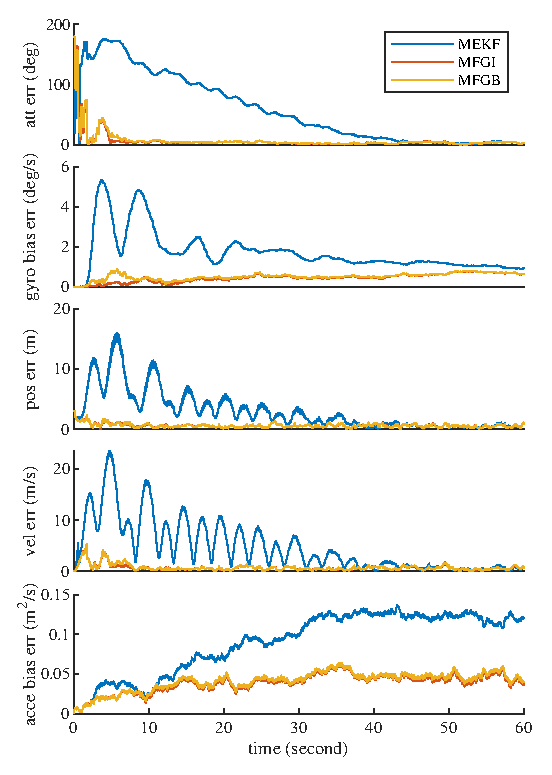
\includegraphics[scale=1.2]{figures/posEst-error}
	\caption{Estimation errors with large initial attitude error.}
	\label{fig:posEst-error}
\end{figure}

\begin{figure}
	\centering
	\begin{subfigure}{\textwidth}
		\centering
		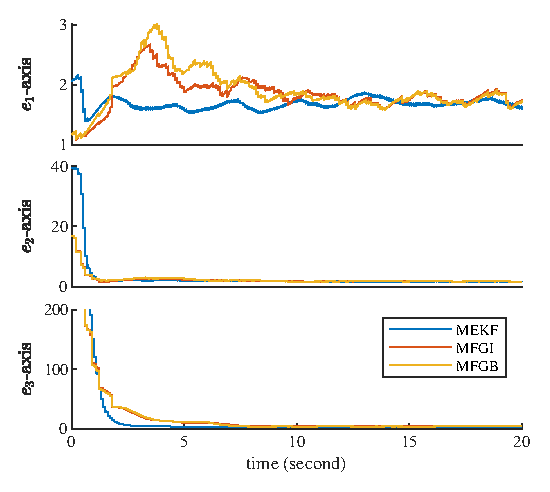
\includegraphics[scale=1.15]{figures/posEst-std-att}
		\caption{Attitude Uncertainty}
		\label{fig:posEst-std-att}
	\end{subfigure}
	\begin{subfigure}{\textwidth}
		\centering
		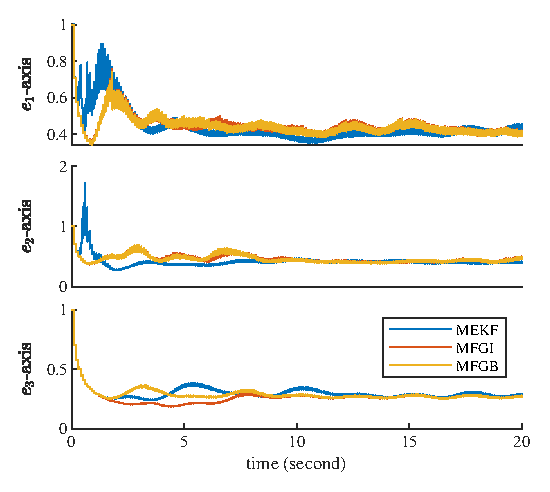
\includegraphics[scale=1.15]{figures/posEst-std-pos}
		\caption{Position Uncertainty}
		\label{fig:posEst-std-pos}
	\end{subfigure}
	\caption{Estimation standard deviation with large initial error.
		The attitude standard deviation for MFG is the square root of the diagonals of $U(\tr{S}I_{3\times 3}-S)^{-1}U^T$, and for MEKF is the square root of the diagonals of the covariance matrix transformed into the inertial frame using the estimated attitude.
		And the position standard deviation is the square root of the corresponding entry in the covariance matrix.}
	\label{fig:posEst-std}
\end{figure}

This is more clearly seen in Figure \ref{fig:posEst-std}, where the estimated standard deviations of the attitude and position are shown.
It is seen that although the MEKF has very large attitude error, its uncertainty is on the same level of MFG filters.
Looking at the attitude standard deviation around the gravity direction (the third row in Figure \ref{fig:posEst-std-att}), it converges exponentially for MEKF, which is typical for an EKF.
On the other hand, it converges slower for the MFG filters, possibly indicating that MFG has better accuracy in modeling large attitude uncertainty, as the attitude dose not converge very fast as indicated in Figure \ref{fig:posEst-error}.
Note that in this IMU-GNSS navigation simulation, the attitude is not directly observed, and it is corrected by its correlation with the position.
This suggests that the MFG not only has better accuracy in attitude uncertainty, but also in the correlation between attitude and position, when the attitude uncertainty is large.

\section{Visual-Inertial Odometry}

\subsection{Pose Estimation Without Map Uncertainty}

\subsection{Numerical Simulations Without Map Uncertainty}

\subsection{Pose Estimation With Map Uncertainty}

\subsection{Numerical Simulations With Map Uncertainty}

